Validation of the Napali approach is intrinsically linked to validation of Makai, both with synthetic benchmarks and in-situ.
Since OPQ utilizes a custom power quality measurement device, its performance needed to be characterized prior to Makai evaluation.

\section{OPQ Box Characterization.}\label{sec:opq-box-characterization.}
A mentioned in Section~\ref{subsec:software} OPQBox generates 4 metrics in order to enable event detection.
In order to evaluate the limits of detection capabilities for each one of these metrics, an OPQBox was fed with synthetic waveform generated by the SDG1025 function generator.
By utilizing a function generator the entire device including the hardware analog front end could be evaluated.
Since the function generator is not capable of supplying $120V_{rms}$ signal, a $120mV_{rms}$ signal was fed on a low side of the OPQBox resistor divider, while the device was powered via an external 5V power supply.

\subsection{Fundamental Frequency}

Fundamental Frequency computation was evaluated by generating a 60Hz sine wave via the SDG1025 and supplying it to the OPQBox.
Calculated frequency was accumulated by analyzing the device triggering stream.
The resulting histogram is shown in Figure~\ref{fig:expdes:1}
\begin{figure}[ht!]
    \begin{center}
        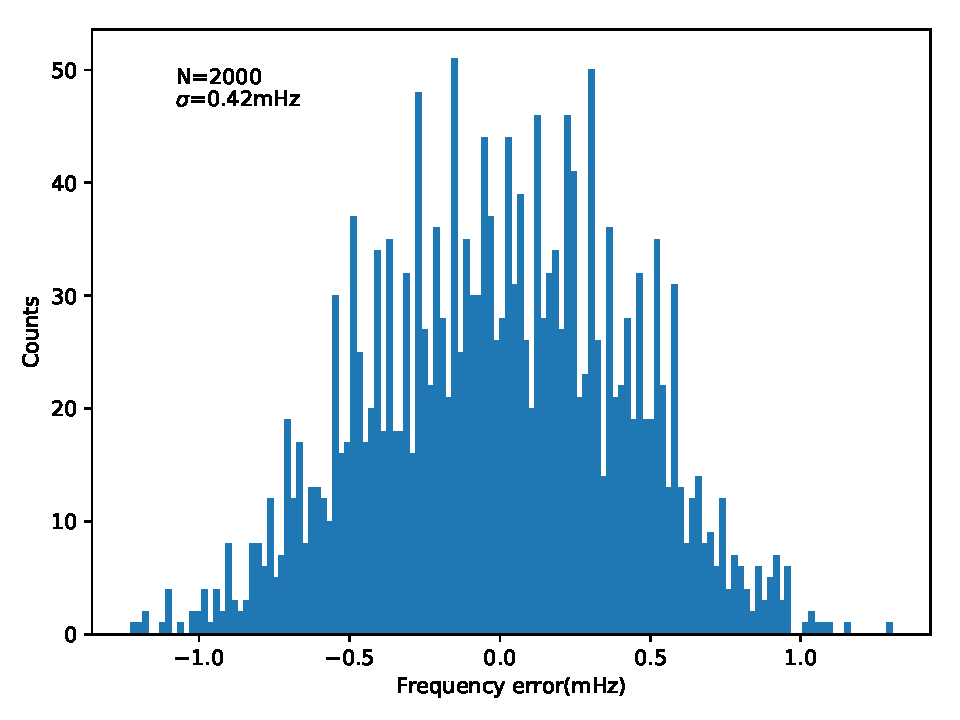
\includegraphics[width=0.6\textwidth]{img/box_eval/frequency_rms.pdf}
    \end{center}
    \caption{OPQBox frequency response.}
    \label{fig:expdes:1}
\end{figure}
As shown, the resulting distribution collected frequencies acquired over 2000s has a $\sigma=420uHz$.

\subsection{Root Mean Square Voltage}
Similarly to the fundamental frequency characterization, $V_{rms}$ calculation was evaluated by supplying the OPQBox with a 60Hz, $120mV_{rms}$ sine wave via the SDG1025.
Calculated RMS was accumulated by analyzing the device triggering stream.
The resulting histogram is shown in Figure~\ref{fig:expdes:2}

\begin{figure}[ht!]
    \begin{center}
        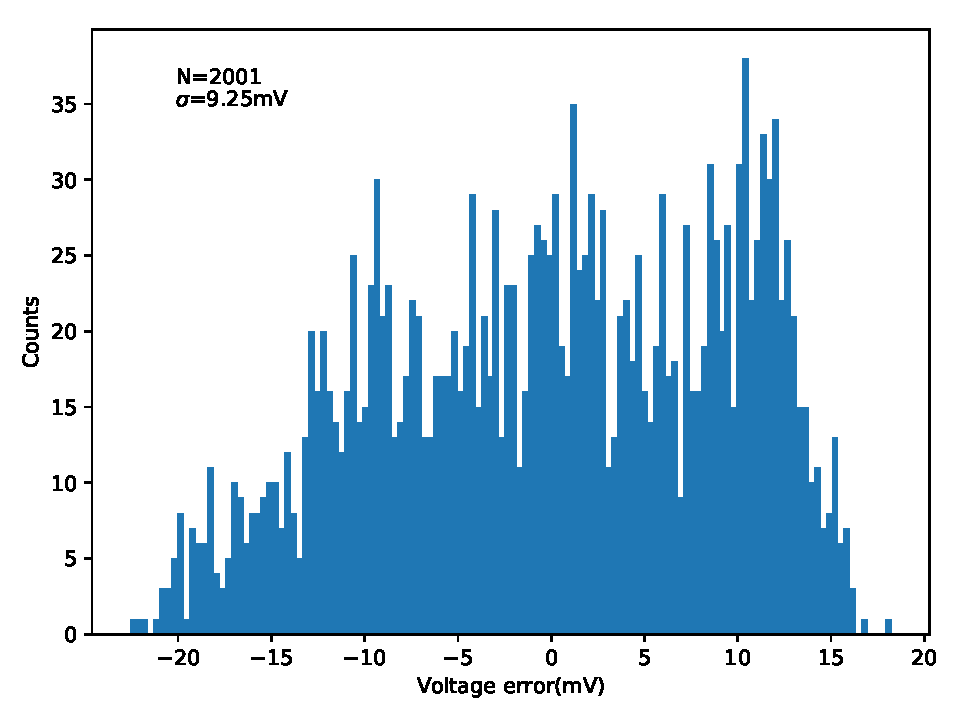
\includegraphics[width=0.6\textwidth]{img/box_eval/rms_histogram.pdf}
    \end{center}
    \caption{OPQBox $V_{rms}$ response.}
    \label{fig:expdes:2}
\end{figure}

As shown, the resulting distribution of collected $V_{rms}$ measurements, acquired over 2000s has a $\sigma=9.34mV$

\subsection{Total Harmonic Distortion}

THD performance of the OPQBox was validated by injecting a various harmonics of 60Hz superimposed onto the 60Hz, $120mV_{rms}$ sine wave into the device via the SDG1025 arbitrary waveform generation capability.
THD calculation results were acquired from the OPQBox triggering stream for analysis.
As expected resultant performance remained self-consistent across all harmonics.
Figure~\ref{fig:expdes:3} shows a histogram of the error in THD values computed from a 60Hz, $120mV_{rms}$ sinewave superimposed with a 240Hz $1.2mV_{rms}$ sine wave.
This measurement is equivalent to $1\%$ THD at the $4^{th}$ harmonic.

\begin{figure}[ht!]
    \begin{center}
        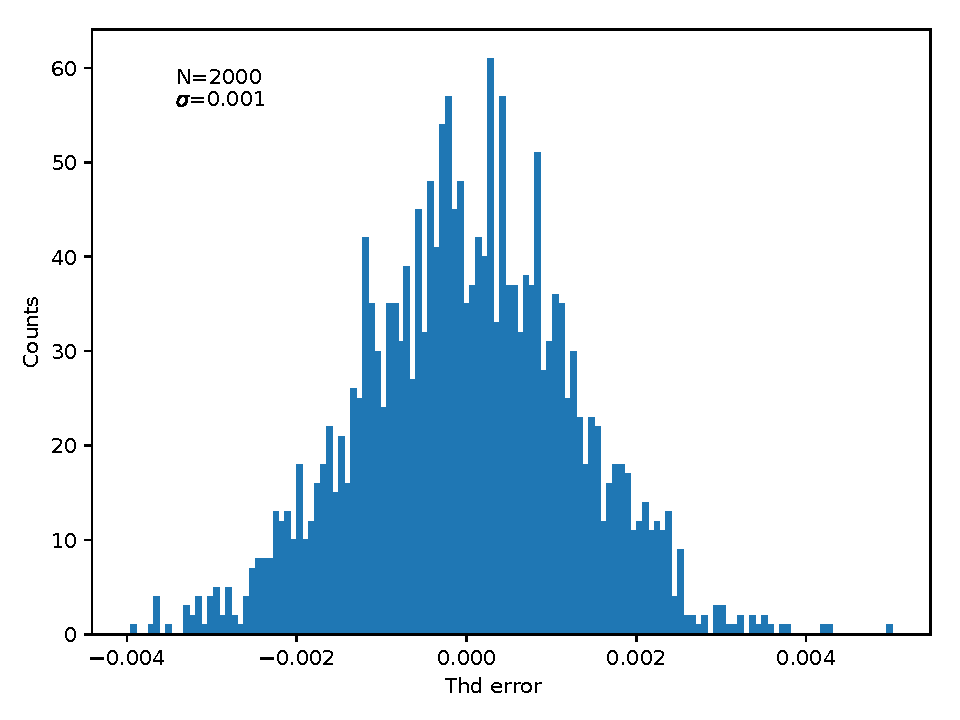
\includegraphics[width=0.6\textwidth]{img/box_eval/thd_rms.pdf}
    \end{center}
    \caption{OPQBox THD response.}
    \label{fig:expdes:3}
\end{figure}

As shown, the resulting distribution of collected THD measurements, acquired over 2000s has a $\sigma=0.001\%$.

\subsection{Transient Detection}

Transient detection performance was evaluated by injecting a transient superimposed onto the 60Hz, $120mV_{rms}$ sine wave into the device via the SDG1025 arbitrary function generation capability.
Transient detection results were acquired by capturing and analyzing the device triggering stream.
Transients of various shapes and magnitudes were tested.

\begin{figure}[ht!]
    \centering
    \begin{subfigure}{.5\textwidth}
        \centering
        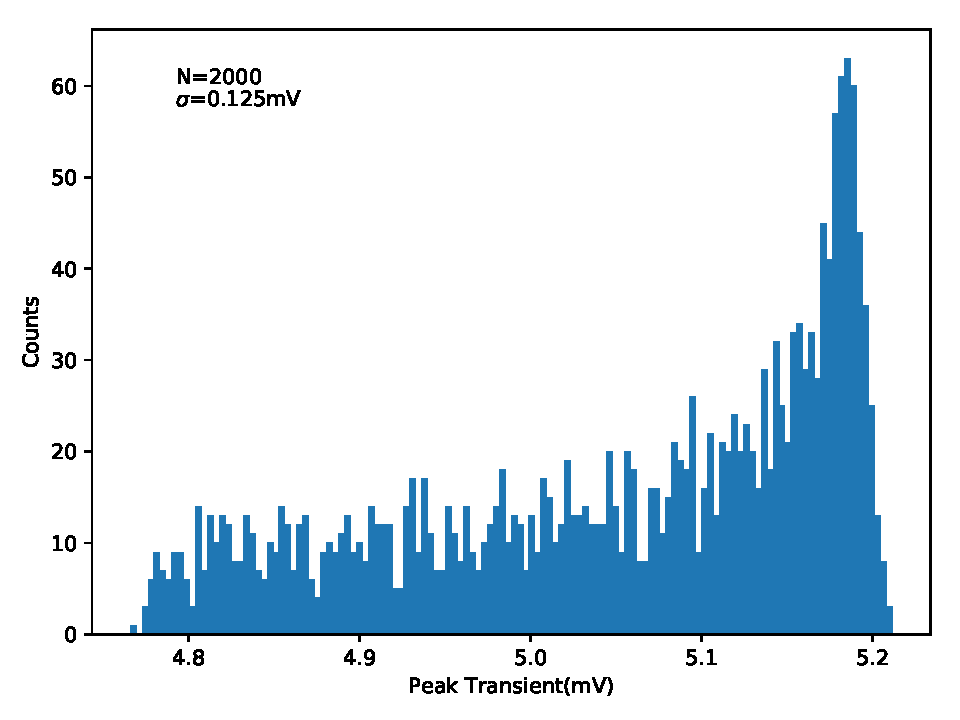
\includegraphics[width=0.9\linewidth]{img/box_eval/5v_transient_rms.pdf}
        \caption{}
        \label{fig:expdes:4:1}
    \end{subfigure}%
    \begin{subfigure}{.5\textwidth}
        \centering
        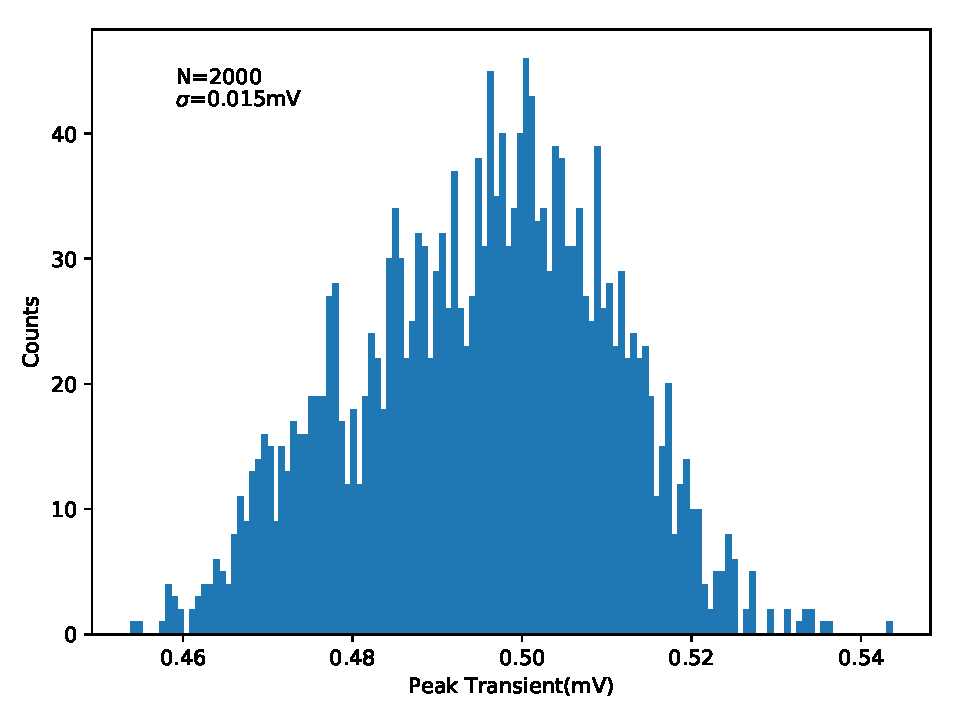
\includegraphics[width=0.9\linewidth]{img/box_eval/0p5v_transient_rms.pdf}
        \caption{}
        \label{fig:expdes:4:2}
    \end{subfigure}
    \caption{Transient detection metric with a 5V transient(a), and 0.5V transient(b)}
    \label{fig:expdes:4}
\end{figure}

Figure~\ref{fig:expdes:4} shows the resultant transient detection metric for two transients.
The shape of the transient is the same and is shown in Figure~\ref{fig:opq:8:3}.
Interestingly, in case of a 0.5V transient the metric results in a much tighter distribution with $\sigma =0.015V$, while in the case of
a 5V transient the distribution exhibits a lower sideband tail.
Since the transient is injected in a random position in the cycle, and the sampling rate of the DG1025 is significantly higher then sampling rate of the OPQBox(25Msps vs 12Ksps), the peak of the transient will sometimes fall in between the consecutive samples of the OPQBox.
In the $0.5V$ transient case this effect is alleviated, since the transient is so small.
Regardless, the result shown in Figure~\ref{fig:expdes:4:2} is presented only as a synthetic benchmark, since OPQBox is expected to operate in an environment with THD larger then $0.4\%$ at $>400Hz$ required to detect a $0.5V$ transient.
As such, the figure of $\sigma=0.125V$ should be considered valid for the OPQBox transient detection capability.
Since this metric is only used in transient detection and not characterization, it was found to be sufficient.
\clearpage
\section{University of Hawaii Deployment.}\label{sec:university-of-hawaii-deployment.2}

As part of the Napali validation, the OPQ system was deployed across the University of Hawaii Manoa campus (UH).
This location was advantageous because it is an isolated microgrid connected to the Oahu powergrid only via a single 46kV feeder as shown in Figure~\ref{expdes:fig:1}.
Another advantage of the UH campus is the high number of smart meters deployed across various levels of the power delivery infrastructure.
While the purpose of these meters is monitoring the power consumption, they do include some rudimentary power quality monitoring capabilities.
Data from the campus deployed meters was used as ground truth for comparison against the measurements, and for analysis performed by the OPQ project.
The location of smart meters in the grid topology is shown in Figure~\ref{expdes:fig:1} as the $M$ nodes.
As evident by the meter location none of them were monitoring the consumer level power and mainly focused on the higher voltage power delivery.
This placement was a consequence of the smart meters role as a consumption monitor, and thus the deployment of the OPQ Boxes at the residential level complimented UH power quality monitoring capabilities without introducing redundancies.

University of Hawaii power grid is supplying a highly diverse infrastructure.
Beyond the traditional residential equipment such as computers and consumer grade electronics, the UH power grid powers scientific and laboratory equipment, machine shops, and server farms.
All of these elements have varying requirements/tolerances for power quality anomalies as well as different levels of power quality ``pollution''.
Furthermore, some of the electricity consumers in the UH campus are entirely unique.
For example, the free electron laser located in the Watanabe Hall is one of the only free electron lasers in the world, and the impact/sensitivity of power quality on the instrument are completely unstudied.
\begin{figure}[ht!]
    \centering
    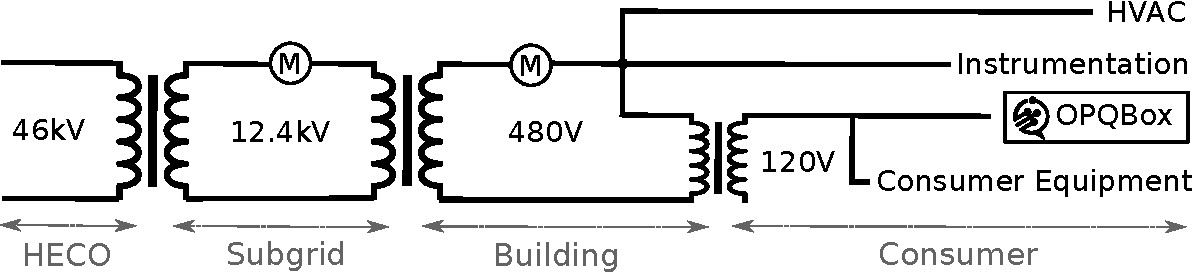
\includegraphics[width=1\linewidth]{img/uh-grid.pdf}
    \caption{University of Hawaii at Manoa power delivery infrastructure.}
    \label{expdes:fig:1}
\end{figure}

There are 74 smart meters deployed across the UH campus.
These meters measured the fundamental frequency $V_{rms}$, power consumption, reactive power, and power factor.
Data from these meters was cross-referenced with the Napali detection system in order to ascertain it's benefits.

OPQ Box placement was specifically selected to cover as much of the University of Hawaii power delivery infrastructure as possible.
The OPQ Box deployment is shown in Figure \ref{expdes:fig:deploy}.
By spreading out devices across the entire power grid, OPQ system is able to monitor the propagation of power quality disturbances throughout the UH power grid.
Consider the event shown in Figure \ref{fig:expdes:9}.
Figure \ref{expdes:fig:grid_wide_filtered} shows the same event with the fundamental and harmonics suppressed using a notch filter bank.
Furthermore, the location annotation is added to indicate the device location.
The most affected devices were located at the Physical Plant and Hamilton Library, recording a $~60V_{pp}$ transient.
Incidentally, both of these devices are monitoring a subgrid rooted at transformer(MA4).
Another device recorded this event was located in Watanabe Hall.
This device recorded a $30V_{pp}$ transient, still above the threshold for detection.
This device was monitoring the the subgrid rooted at the transformer LA4.
The final device was located at the parking structure entirely across campus.
This device recorded a $15V_{pp}$ transient, about 1V below the required magnitude for the threhold based detection.
However, Napali was able to determine that the parking structure OPQ Box was affected by the disturbance, and requested the raw data regardless.

\begin{figure}[ht!]
    \centering
    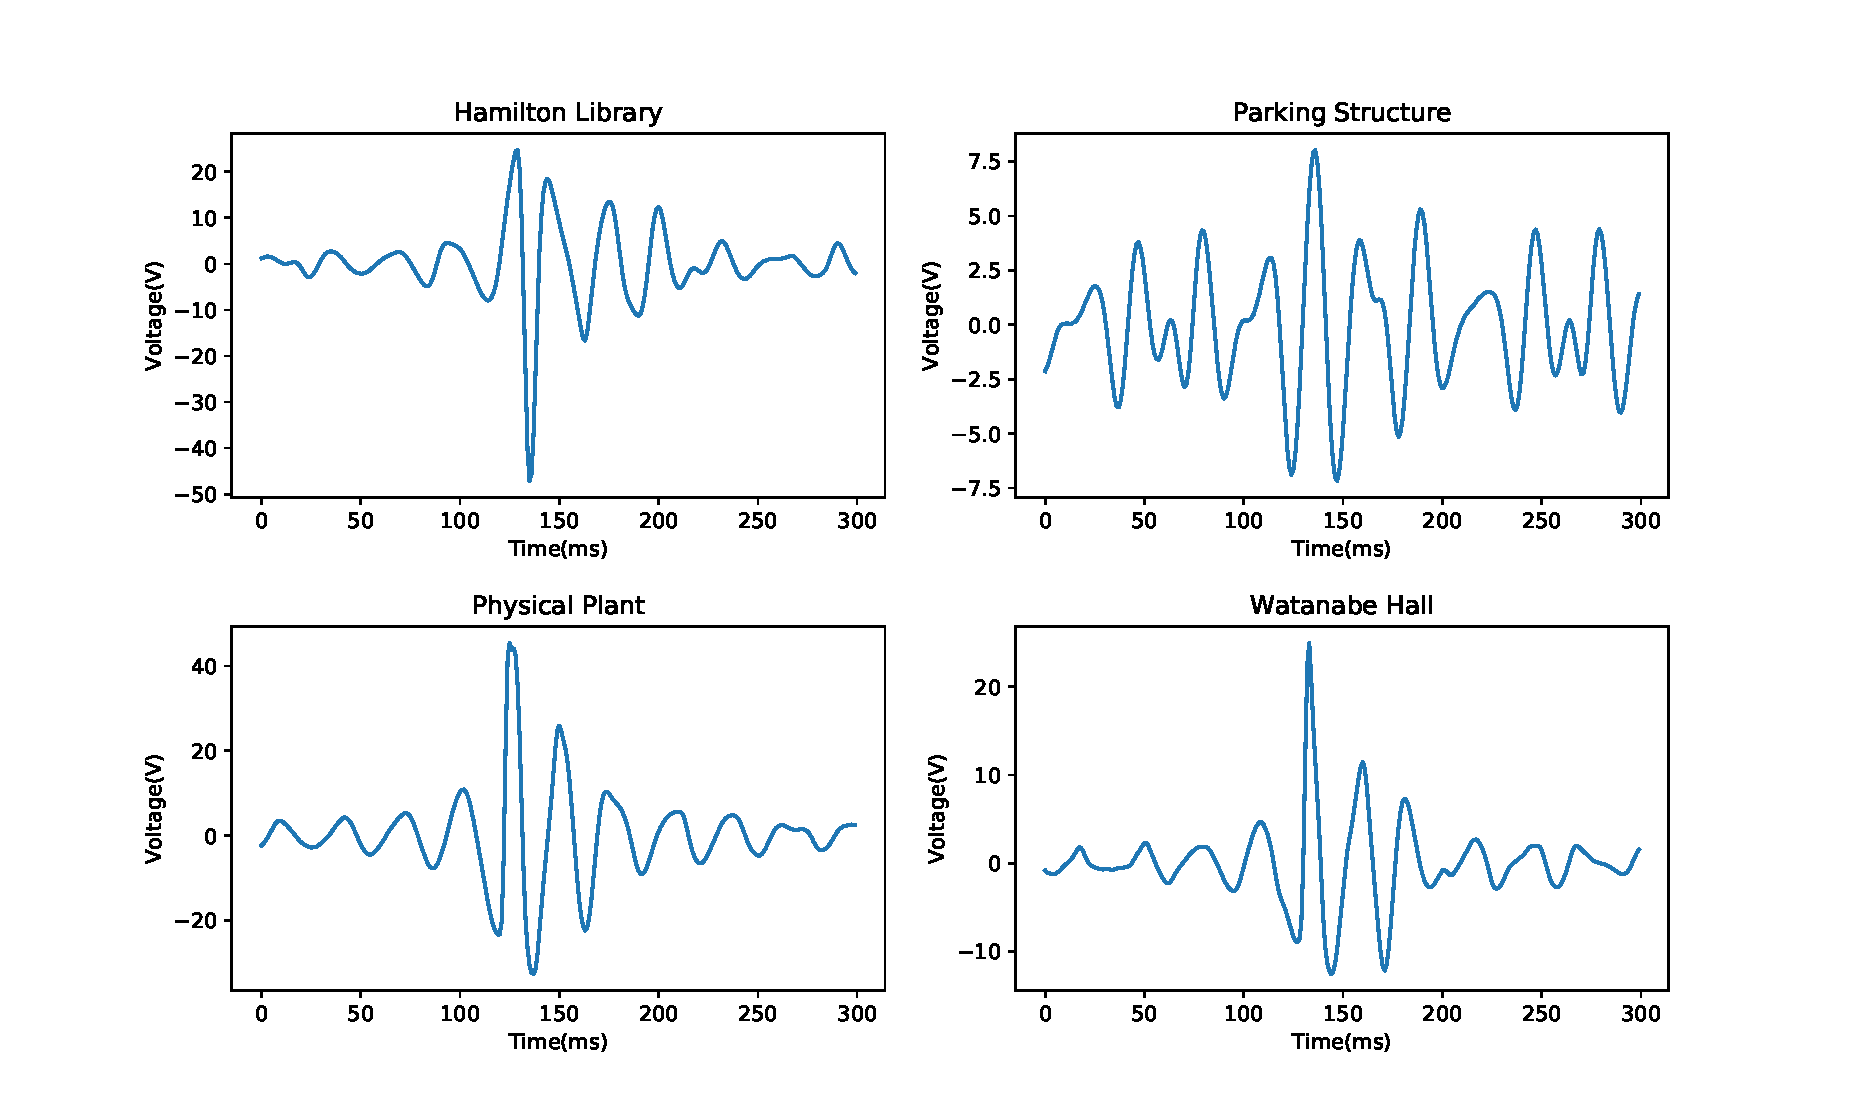
\includegraphics[width=1\linewidth]{img/deployment/gridwide_locality.pdf}
    \caption{Filtered Transient from event shown in Figure \ref{fig:expdes:9}}
    \label{expdes:fig:grid_wide_filtered}
\end{figure}

From the data gathered by Napali as shown in Figure \ref{expdes:fig:grid_wide_filtered}, it seems apparent that the disturbance originated at the subgrid rooted at the transformer MA4.
The Watanabe device was affected due to the short geographic and electrical distance to the MA4 subgrid.
By the time transient reached the parking structure, it was significantly attenuated by the transformers and transmission lines.
It was only detected due to the sub-threshold detection ability of the Napali framework.

\begin{figure}[H]
    \centering
    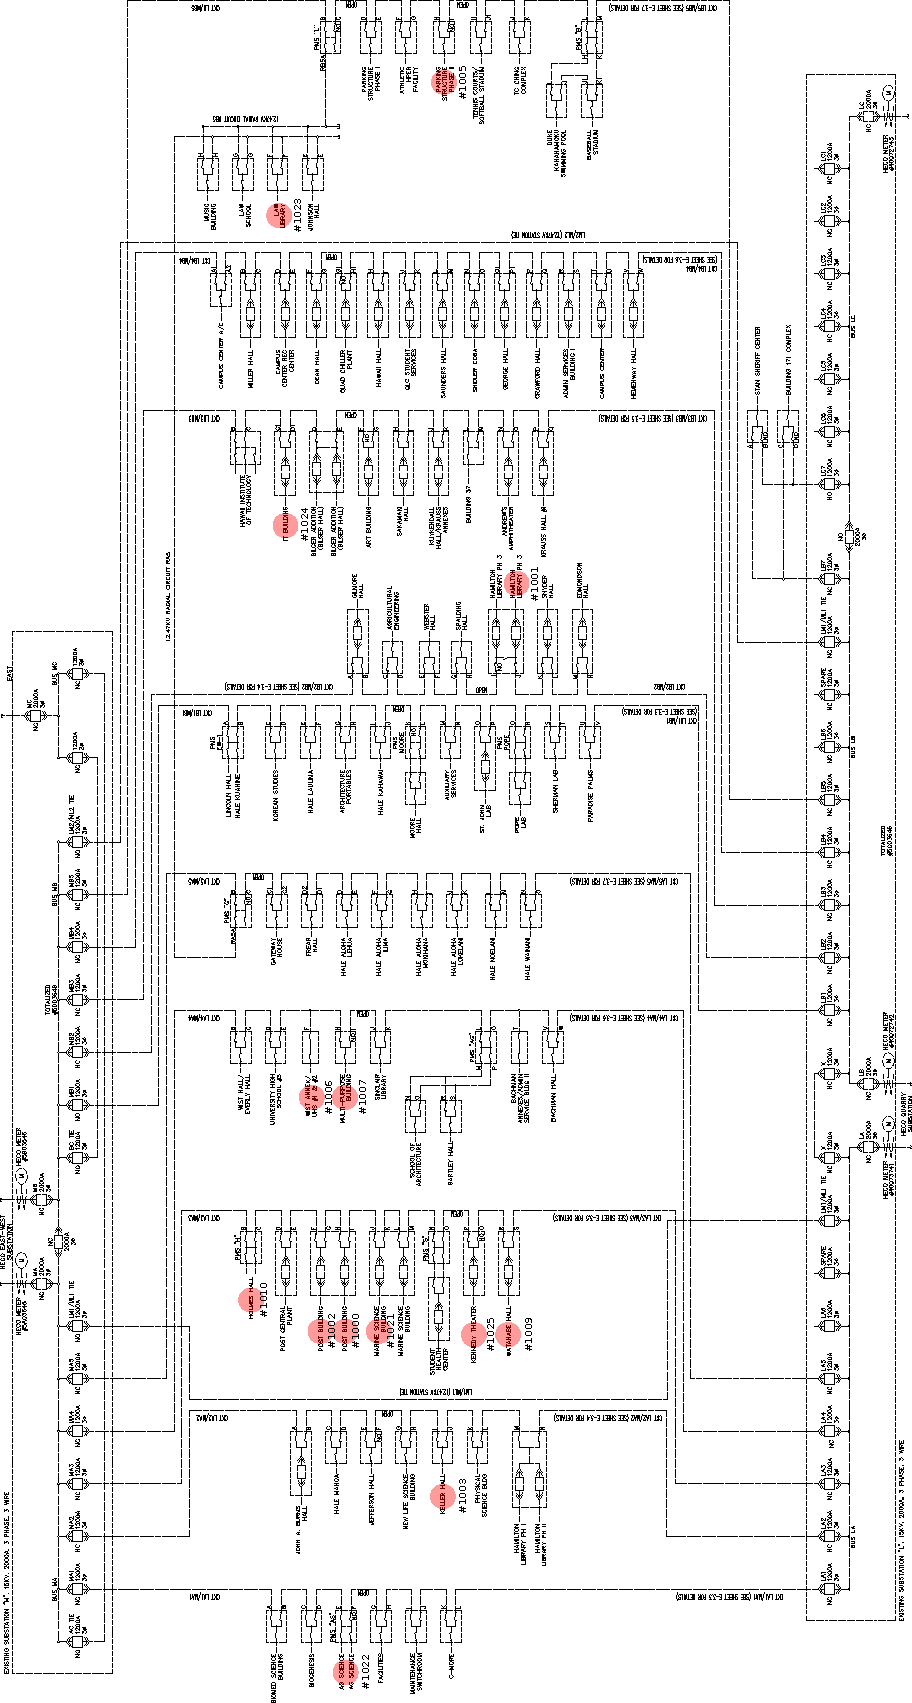
\includegraphics[width=0.7\linewidth]{img/deployment/uh_power_grid.pdf}
    \caption{OPQ Box locations and device IDs across University of Hawaii.}
    \label{expdes:fig:deploy}
\end{figure}
\clearpage
\subsection{Selection of $\alpha$ parameter}\label{subsec:selectrion-ofparameter}

The main tunable parameter in Napali is the $\alpha$ coefficient used in the low pass filter as shown in Equation \ref{eq:iir_mean}.
This parameter determines the memory of the lowpass filter used in the calculation of the mean and the standard deviation of metrics from OPQBox data stream.
These statistics are in turn used during the Napali triggering process to locate sub-threshold gridwide events.

A smaller $\alpha$ parameter corresponds to a longer memory in the low pass filter as shown in Equation \ref{eq:iir_alpha}.
This is further visualized in Figure \ref{fig:expdes:5}.
In particular this Figures \ref{fig:expdes:5:1} and \ref{fig:expdes:5:2} show the response of the IIR low pass filter to the simulated frequency measurements.
The dashed red line represents the frequency measurement, solid red line represents the filtered mean, and the blue line represents the standard diviation.
Figures \ref{fig:expdes:5:1} shows the filter response for $\alpha = 0.5$ or $T_{memory} \approx 10s $.
As evident from the plot, the mean and the standard deviation quickly recover from the transient are return to their nominal values.
Furthermore, the mean is closely tracking the random fluctuations present in the measurement.
Figures \ref{fig:expdes:5:1} shows the filter response for $\alpha = 0.05$ or $T_{memory} \approx 123s $.
While the stimuli remains the same, it takes significantly longer the statistics to recover.
Additionally, the mean no longer tracks the frequency fluctuations present in the simulated data.
\begin{figure}[ht!]
    \centering
    \begin{subfigure}{0.9\textwidth}
        \centering
        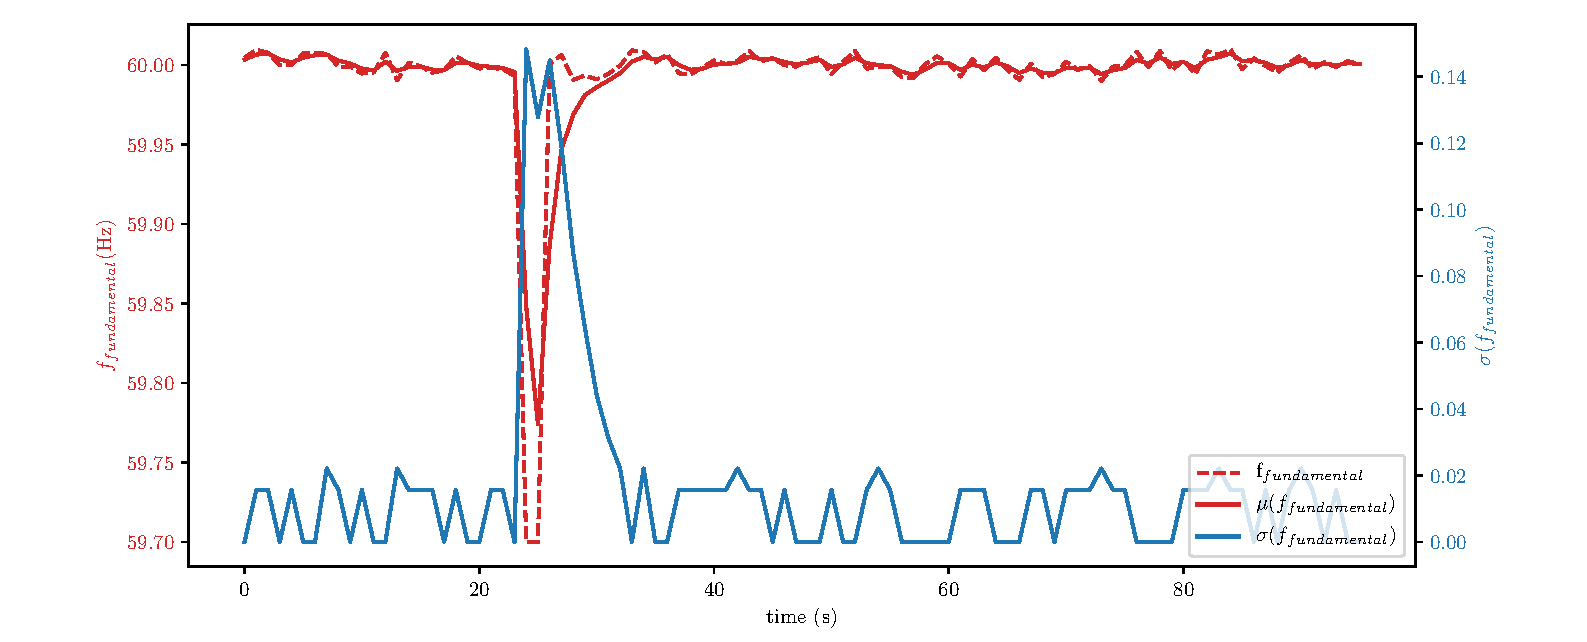
\includegraphics[width=1\linewidth]{img/napali_eval/Napali_response_freq_05.pdf}
        \caption{}
        \label{fig:expdes:5:1}
    \end{subfigure}%

    \begin{subfigure}{0.9\textwidth}
        \centering
        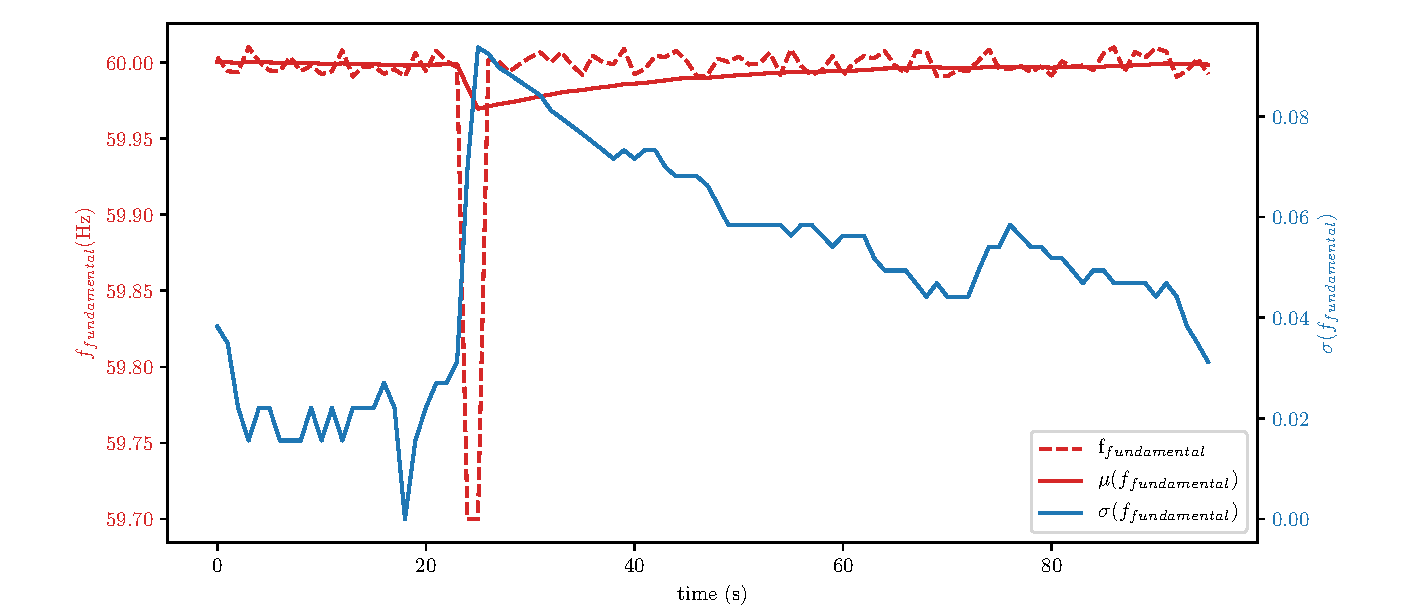
\includegraphics[width=1\linewidth]{img/napali_eval/Napali_response_freq_005.pdf}
        \caption{}
        \label{fig:expdes:5:2}
    \end{subfigure}
    \caption{$\mu$ and $\sigma$ behaviour with a)$\alpha = 0.5$ and b)$\alpha=0.05$}
    \label{fig:expdes:5}
\end{figure}

Picking the $\alpha$ parameter for Napali is extremely domain specific, as it depends on the frequency content of the triggering stream.
Intuitively, the $T_{memory}$ parameter needs to be long enough to adjust to gradual changes in the triggering stream for the mean calculation,
and dampen the standard deviation for detection of multiple consecutive anomalies.
In addition, it needs to be short enough to converge on the mean and the standard deviation during a step-like transition in the triggering stream.

Luckily, in the Power Quality domain the Napali $\alpha$ selection is fairly forgiving.
This is demonstrated in Figure \ref{fig:expdes:6}.
This graph represents the amount of time that Napali considered one of the metrics to be outside of the $3\sigma$ of the mean for various values of $\alpha$.
The triggering stream used to generate these values was captured over 24 hours by one of the OPQBoxes deployed on the University of Hawaii campus.
All devices deployed thus far have followed a similar pattern.
With $20s <T_{memory} < 2Hr$ the triggering stream resulted in similar behaviour, with the system correctly marking all potential sub-threshold events.
At $T_{memory} \approx 20s$, system quickly recovered from large jumps in the triggering stream, however it marked a significant number of small anomalies ($\Delta_{f}>0.01Hz$, $\Delta_{v}> 0.1V$\ldots etc) as outside $3\sigma$, and thus candidates for sub-threshold events.
At $T_{memory} \approx 2Hr$, system took  significant amount of time to recover from large jumps in triggering metrics, thus marking the metric as outside of $3\sigma$ for many tens of minutes.
Furthermore, some of the larger anomalous measurements ($\Delta_{f}>0.05Hz$, $\Delta_{v}> 2V$\ldots etc) were no longer flagged as sub-threshold candidates.
Outside of the two extremes, the system behaviour was quite similar.
During all of the deployments the OPQ system was operating with:
\begin{equation}\label{eq:opq_alpha}
\begin{aligned}
    \alpha = 0.05
\end{aligned}
\end{equation}


Which corresponds to the $T_{memory} \approx 2$ minutes.
Thresholds which initiate the Napali event detection state machine are shown in Table \ref{tbl:opq:thresholds}.
\begin{figure}[ht!]
    \centering
    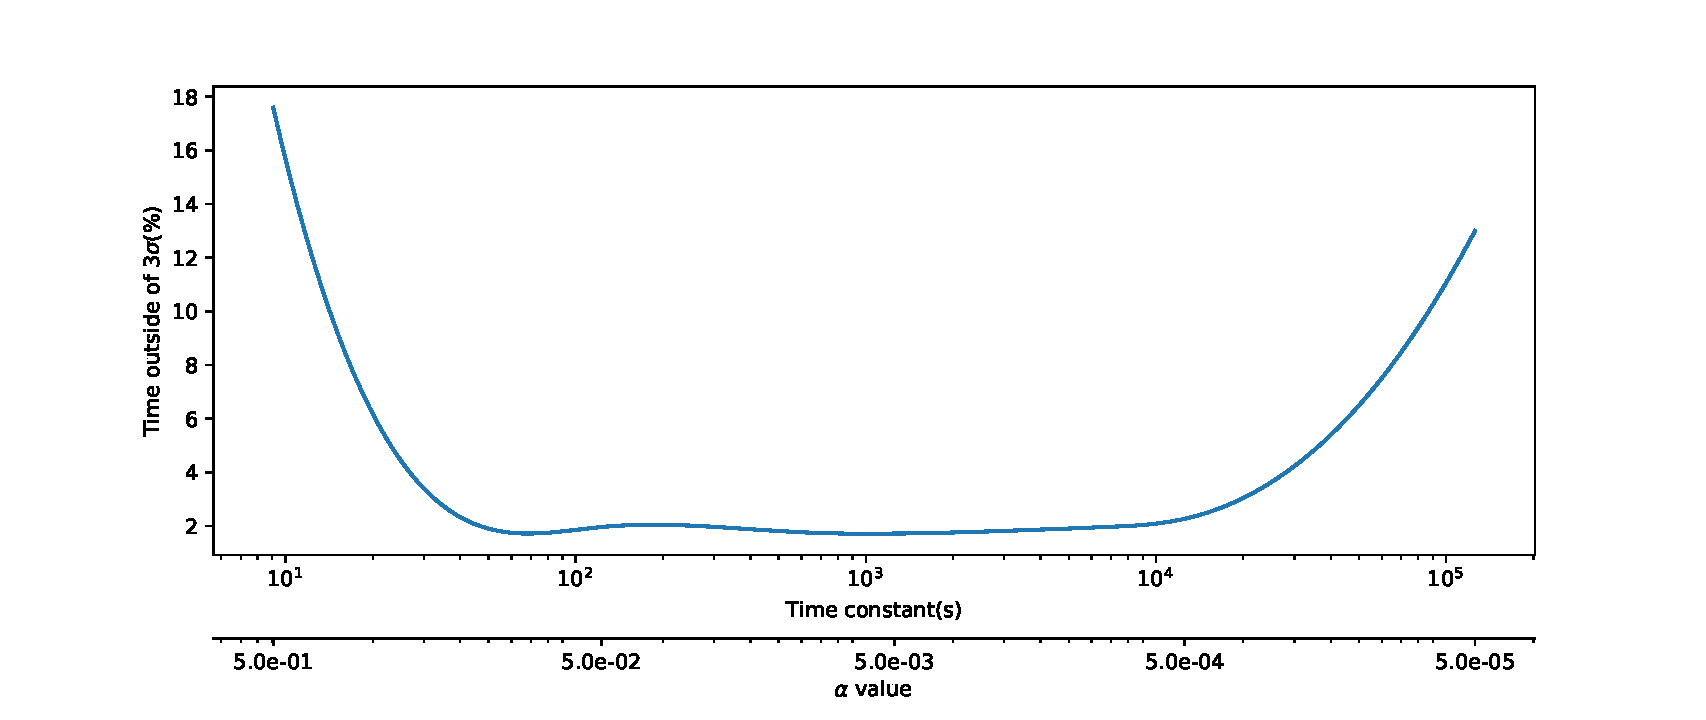
\includegraphics[width=1\linewidth]{img/napali_eval/a_selection.pdf}
    \caption{Amount of time a metric spends outside of the $3\sigma$ for various values of $\alpha$}
    \label{fig:expdes:6}
\end{figure}

The effect of the of selecting alpha as shown in Equation \ref{eq:opq_alpha} can be observed in Figure \ref{fig:expdes:7}.
This figure shows interesting features from the same dataset that was used to produce Figure \ref{fig:expdes:6}.
Blue traces show metrics that exhibit anomalous behaviour, while red indicates that Napali has flagged this temporal region as a sub-threshold event candidate.
Figure \ref{fig:expdes:7:1} shows a frequency fluctuation which nearly passes the threshold of $60.1Hz$ which would mark it as a full fledged event.
Instead, Napali marked almost the entirety of the fluctuation as a potential sub-threshold event, as shown by the red trace.
Figure \ref{fig:expdes:7:2} shows a step in the total harmonic distortion metric, similar to the one shown in Figure \ref{fig:opq:7} at the 6am mark.
In this case the metric in question abruptly changed to a new mean, requiring a fairly slow $\alpha$ coefficient to catch up over 3 minutes.
While it may seem wasteful to mark large temporal regions following an abrupt jump as candidates for sub-threshold event, it is important to note that:
\begin{enumerate}
    \item Making the $\alpha$ parameter smaller does not benefit the false positive rate as shown in Figure \ref{fig:expdes:6}.
    \item In-situ there is no way to tell if an abrupt shift is a switch to a new steady state, or if the metric will recover to a previous mean.
\end{enumerate}
It is important to remember than Napali is not meant to have a low false positive rate.
Instead, a system like OPQ Mauka can use all available information, including the raw data, to determine if an event is true gridwide event with much higher confidence.
The main goal of Napali is to have an extremely low rate of false negatives.
Figure \ref{fig:expdes:7:3} is on a different timescale from Figures \ref{fig:expdes:7:2} and \ref{fig:expdes:7:1}.
This is done in order to include several potential sub-threshold events into a common chart.
Five temporal regions during the the 3 Hrs are marked by Napali as potential sub-threshold events.
\begin{figure}[ht!]
    \centering
    \begin{subfigure}{0.5\textwidth}
        \centering
        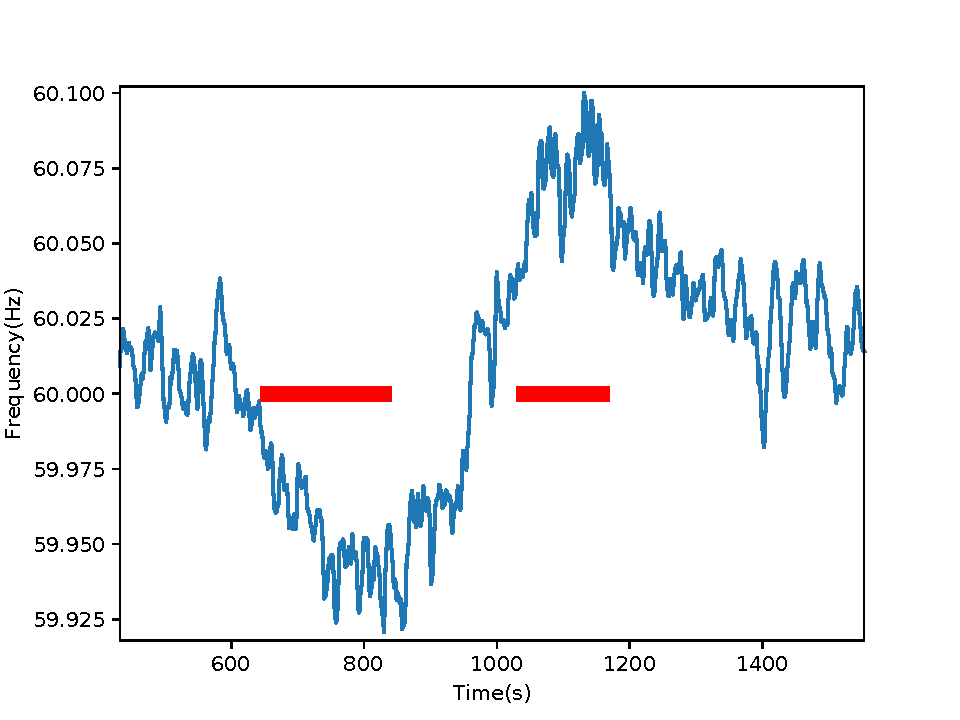
\includegraphics[width=1\linewidth]{img/napali_eval/napali_live_f.pdf}
        \caption{}
        \label{fig:expdes:7:1}
    \end{subfigure}%
    \begin{subfigure}{0.5\textwidth}
        \centering
        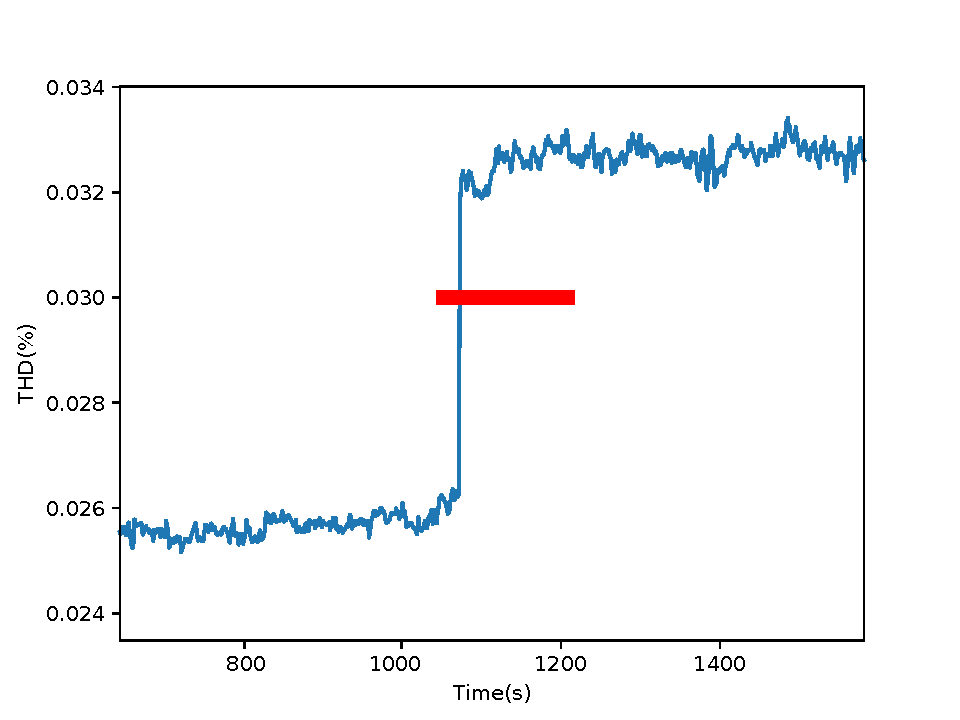
\includegraphics[width=1\linewidth]{img/napali_eval/napali_live_thd.pdf}
        \caption{}
        \label{fig:expdes:7:2}
    \end{subfigure}

    \begin{subfigure}{0.5\textwidth}
        \centering
        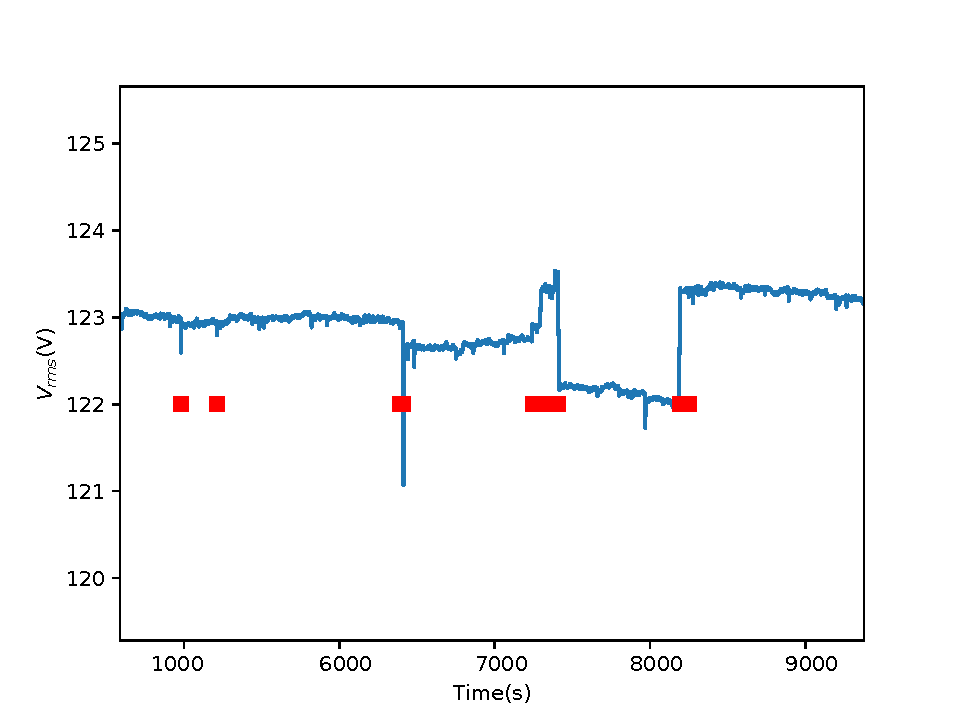
\includegraphics[width=1\linewidth]{img/napali_eval/napali_live_rms.pdf}
        \caption{}
        \label{fig:expdes:7:3}
    \end{subfigure}

    \caption{Potential sub-threshold events for a) $f_{fundamental}$, b)$THD$, and c)$V_{rms}$
    Red boxes indicate that Napali picked these temporal windows as a potential sub-threshold event.}
    \label{fig:expdes:7}
\end{figure}

\subsubsection{Deployment nomenclature}\label{subsec:deploynment-nomenclature}
In this section I describe the nomenclature used throughout Napali evaluation.
Since this deployment is unique, naming convention of particular deployment characteristics and events is unique to this paper.

\begin{figure}[ht!]
    \centering
    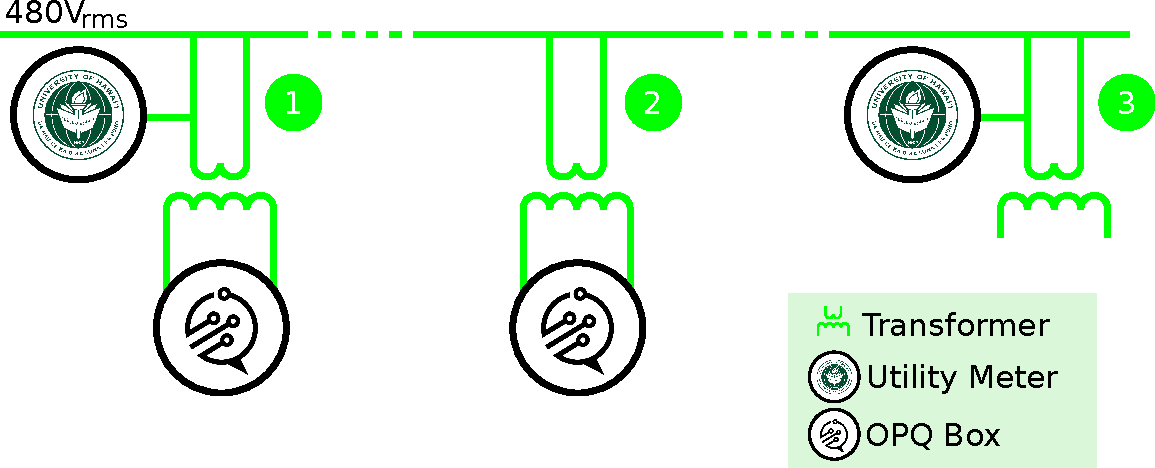
\includegraphics[width=1\linewidth]{img/deployment/meter_types.pdf}
    \caption{Three categories of device deployments.}
    \label{fig:expdes:nomenclature}
\end{figure}

All meters, both Utility and OPQ Box fall into three categories shown in Figure \ref{fig:expdes:nomenclature}.
Category 1 are collocated devices.
In this situation the Utility meter is monitoring the the $480V_{rms}$ three phase line going into the building.
A transformer converts the $480V_{rms}$ to the household $120V_{rms}$.
A deployed OPQ Box monitors the $120V_{rms}$ line.
This category of devices is particularly important because they provide a baseline for comparison between the OPQ Box performance and a commercially installed system.
The second category of deployed devices are the non-collocated OPQ Boxes.
These devices are deployed in buildings that lack smart meters.
Thus, we lack ground truth data for these devices.
However, these devices are still useful for subthreshold triggering studies.
Finally, category 3 consists of non-collocated Utility meters.
These meters monitor locations without a deployed OPQ device.
Similarly to locations in category 2, data from these devices proved useful in subthreshold event detection evaluation.

There are several types of events that Napali was able to detect.
First category are gridwide events.
Gridwide events effect every device on the OPQ network, with each device passing one of the designated threshold threshold.
Gridwide events inherently lack a subthreshold component since every device capture over-threshold data.
Partial gridwide events events that affected only a subset of devices enough to trigger pass the threshold.
One of the main goals of Napali is to utilize metric extraction in order to detect sub-threshold events.
During the deployment, two types of sub-threshold events have been identified:
\begin{itemize}
    \item Partial sub-threshold event.
    \item Full sub-threshold event.
\end{itemize}
Full sub-threshold events consist of one or several devices passing the threshold described in Table \ref{tbl:opq:thresholds},
as well as one or several devices marked as sub-threshold by Napali.
Partial sub-threshold events consist of devices which all passed the threshold described in Table \ref{tbl:opq:thresholds}, however some of the devices triggered on a different metric with a much shorter temporal window.
The important distinction between partial sub-threshold events and regular events is that if triggered using the Self-Triggering method, the majority of the sub-threshold data would be lost.

One would expect that partial gridwide events would be divided into those with and without a subthreshold component,
however, none of the events captured by Napali during the deployment consist of only over-threshold waveforms.
As such, all of the Napali partial gridwide events are also subthreshold events, and the term is used interchangeably.

\begin{figure}[ht!]
    \centering
    \begin{subfigure}{1\textwidth}
        \centering
        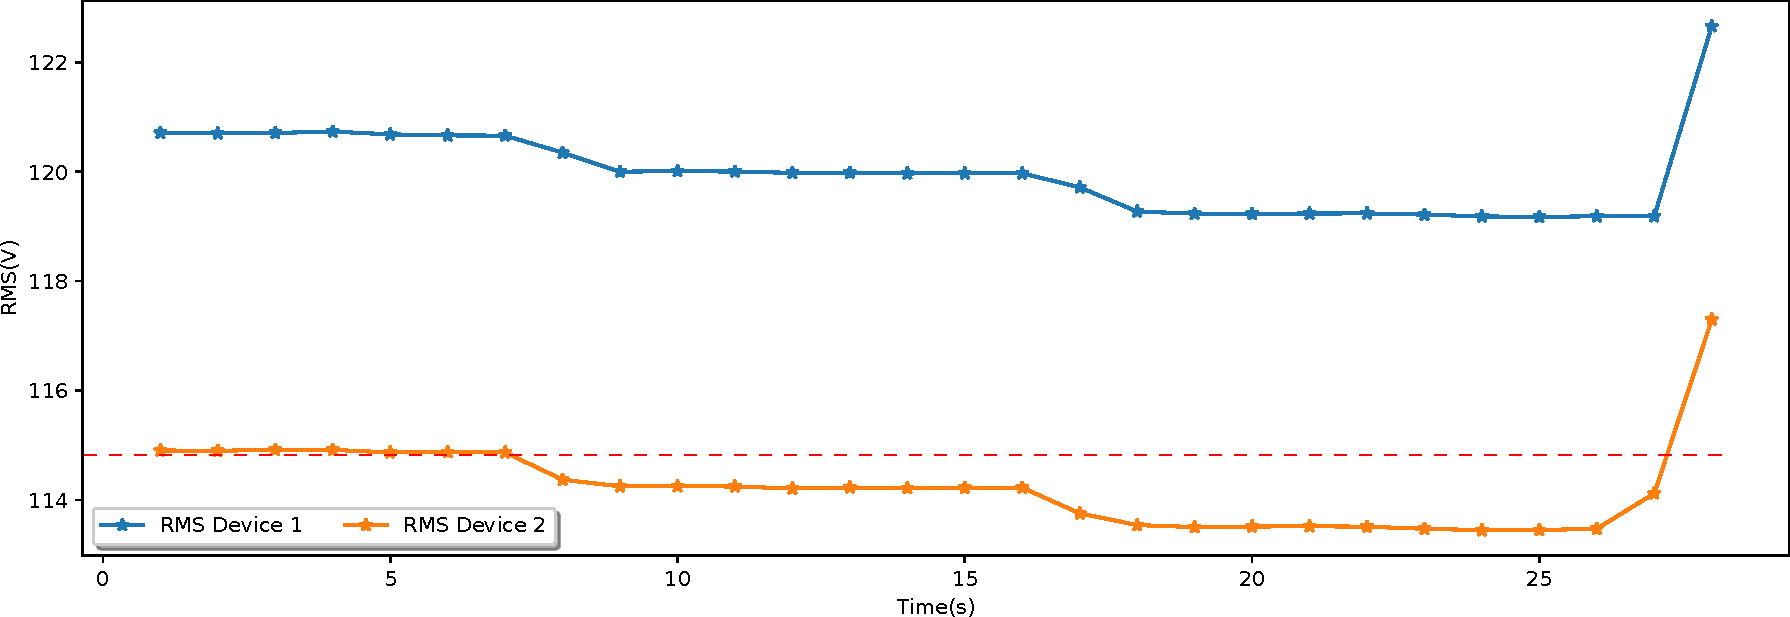
\includegraphics[width=1\linewidth]{img/napali_eval/rms_gridwide_subthreshold.pdf}
        \caption{}
        \label{fig:expdes:8:1}
    \end{subfigure}%

    \begin{subfigure}{1\textwidth}
        \centering
        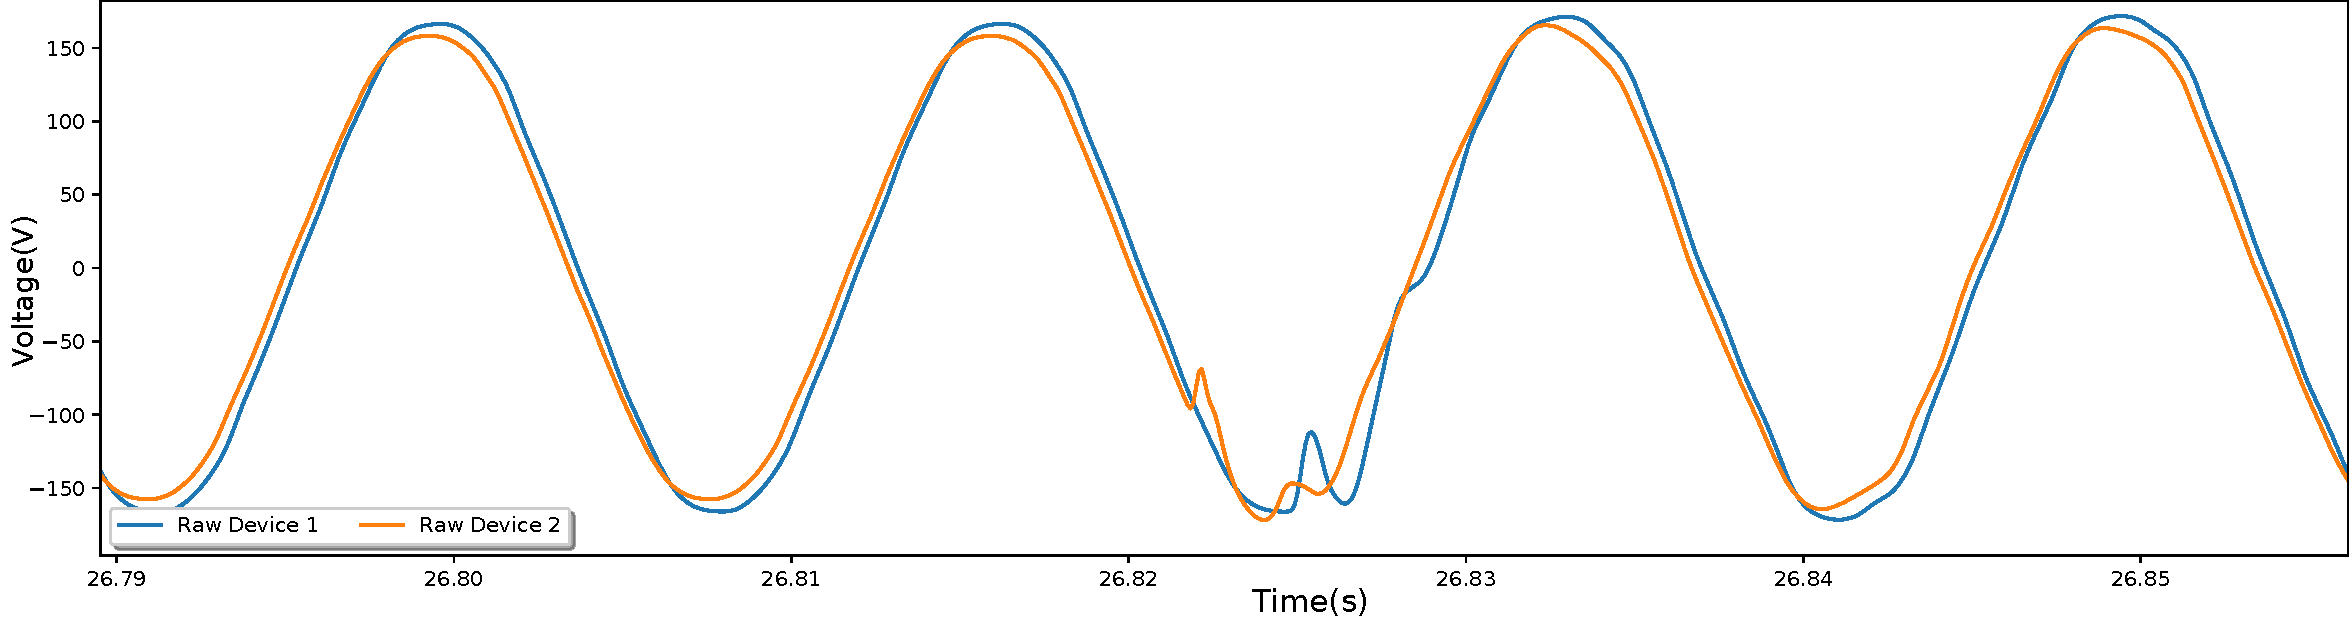
\includegraphics[width=1\linewidth]{img/napali_eval/raw_gridwide_subthreshold_zoom.pdf}
        \caption{}
        \label{fig:expdes:8:2}
    \end{subfigure}
    \caption{Partial sub-threshold event a) the sub-threshold component of the event, b) above threshold component of the event}
    \label{fig:expdes:8}
\end{figure}

An example of a partial sub-threshold event is shown in Figure \ref{fig:expdes:8}.
Figure \ref{fig:expdes:8:1} shows the sub-threshold component of the event.
In this event device 2 passed the threshold on $V_{rms}$ metric, initiating Napali to look for sub-threshold events across other devices.
It is important to note, that at the event start device 1 was considered to be a sub-threshold candidate, however, at $t \approx 26.8s$ device 1 produced a transient metric which was above Napali threshold.
As such Napali requested raw data from both device 1 and device 2, creating a partial sub-threshold event containing both a voltage sag shown in Figure \ref{fig:expdes:8:1} and a transient shown in Figure \ref{fig:expdes:8:2}.

\begin{figure}[ht!]
    \centering
    \begin{subfigure}{0.49\textwidth}
        \centering
        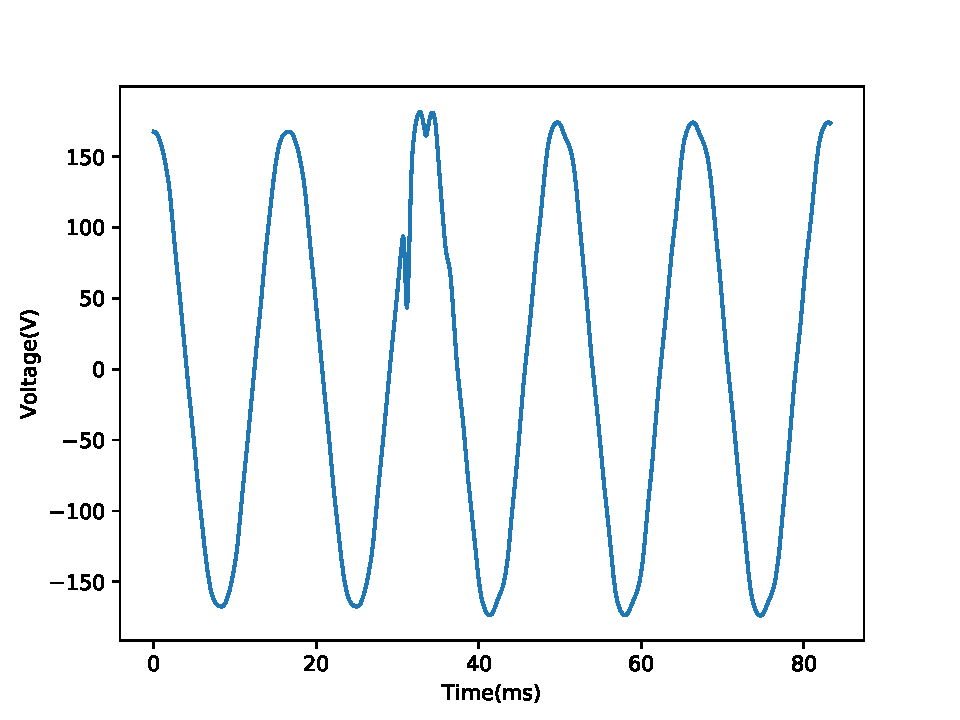
\includegraphics[width=1\linewidth]{img/napali_eval/raw_gridwide_sub_full1.pdf}
        \caption{}
        \label{fig:expdes:9:1}
    \end{subfigure}%
    \begin{subfigure}{0.49\textwidth}
        \centering
        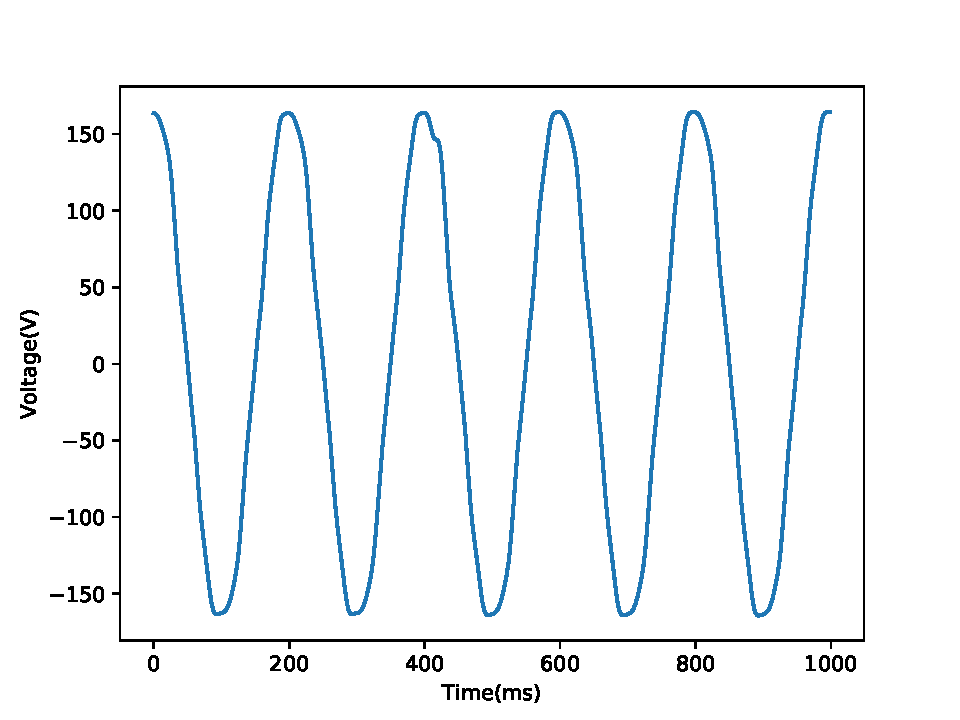
\includegraphics[width=1\linewidth]{img/napali_eval/raw_gridwide_sub_full2.pdf}
        \caption{}
        \label{fig:expdes:9:2}
    \end{subfigure}

    \begin{subfigure}{0.49\textwidth}
        \centering
        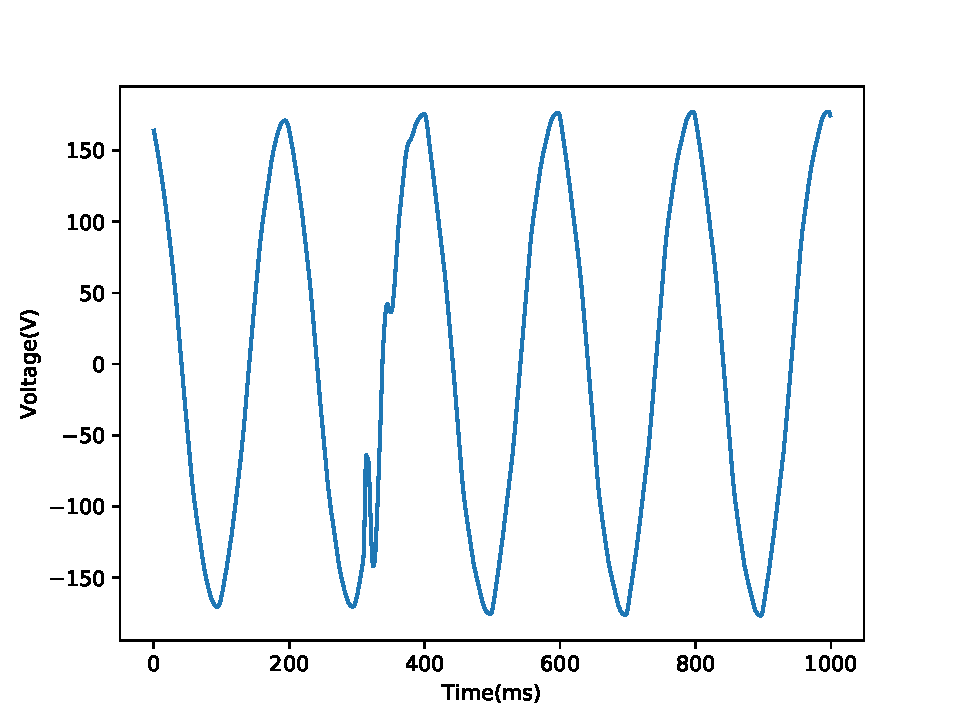
\includegraphics[width=1\linewidth]{img/napali_eval/raw_gridwide_sub_full3.pdf}
        \caption{}
        \label{fig:expdes:9:3}
    \end{subfigure}
    \begin{subfigure}{0.49\textwidth}
        \centering
        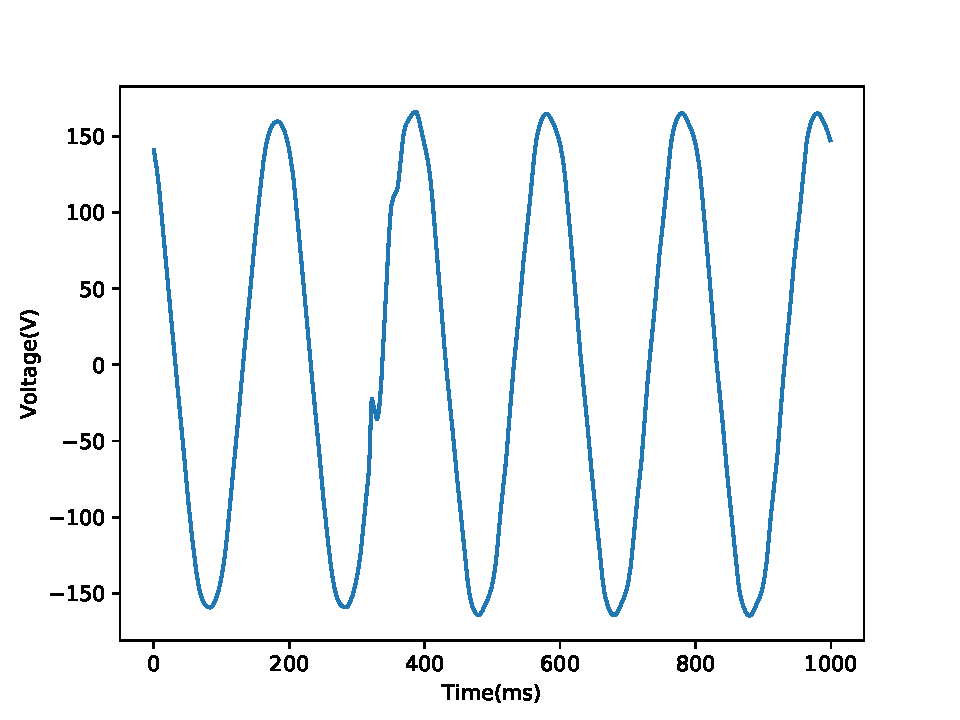
\includegraphics[width=1\linewidth]{img/napali_eval/raw_gridwide_sub_full4.pdf}
        \caption{}
        \label{fig:expdes:9:4}
    \end{subfigure}
    \caption{Full sub-threshold event across 4 devices.
    a) Device 1: above threshold b) Device 2: sub-threshold c) Device 3: above threshold d) Device 4: above threshold.}
    \label{fig:expdes:9}
\end{figure}

An example of a full sub-threshold event is shown in Figure \ref{fig:expdes:9}.
This is a short-lived transient event observed by four devices on September 5\textsuperscript{th}.
Devices 1, 3, and 4 generated a transient metric higher then the Napali threshold.
Device 2 transient metric did not pass threshold, yet nonetheless produced a severe enough deviation from the mean for Napali to consider it a part of the event.
This is particularly evident in the mild transient observed in Figure \ref{fig:expdes:9:2}.

\subsection{Event Dataset}\label{subsec:event-dataset}
Event dataset used in this analysis consists of data from 15 devices collected between November 14th and January 1st 2019.
There are 2163 events in total, with 1378 $V_{rms}$ events and  737 transient events.
6 Events were related solely to frequency and 83 related solely to total harmonic disturbance.
During the deployment, OPQ network achieved 97\% availability with only downtime relating to software updates and a power outage November 25h power outage.


\clearpage

\section{Napali Validation}\label{sec:napali-validation}

Napali was validated using simulation, synthetic data with the device-in-loop, and in-situ during the deployment.
Throughout this section I validate the claims of my dissertation as outlined in Section \ref{intro:sec:claim}.

\subsection{Napali Bandwidth usage}\label{subsec:napali-bandwidth-usage}
During the OPQ deployment it was found that Napali significantly outperformed both the Self-Triggered and the Naive event detection methods.
In order to evaluate the bandwidth performance of Napali a Self-Triggered plugin ran along side it inside the Makai host.
This plugin utilized the same thresholds as Napali as described in Table \ref{tbl:opq:thresholds}.
However, the Self-Triggered plugin did not take into the account any inter-device signatures.
This method is equivalent to each the device performing non-collaborative triggering.
\begin{figure}[ht!]
    \centering
    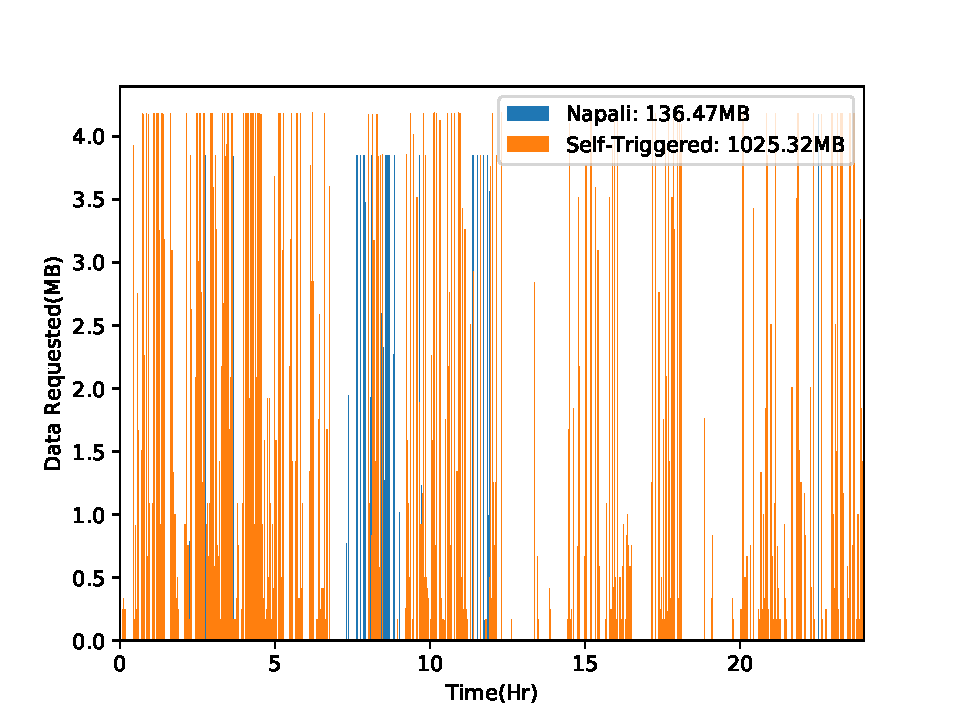
\includegraphics[width=0.8\linewidth]{img/napali_eval/napali_request_bandwidth.pdf}
    \caption{Amount of data requested from 10 OPQ Boxes via the Self-Triggered and Napali methods.}
    \label{expdes:fig:self_triggered_bandwidth}
\end{figure}

Figure \ref{expdes:fig:self_triggered_bandwidth} shows the amount of data requested from 10 devices by the Self-Triggered and Napali plugins over 24 Hours.
It is evident, that the majority of data requests for the Self-Triggered method resulted in local noise, and did not contribute to the grid measurements.
Napali on the other hand, ignored anomalies which did not affect more then a single device, while requesting sub-threshold data during a gridwide PQ event.

\begin{figure}[ht!]
    \centering
    \begin{subfigure}{.5\textwidth}
        \centering
        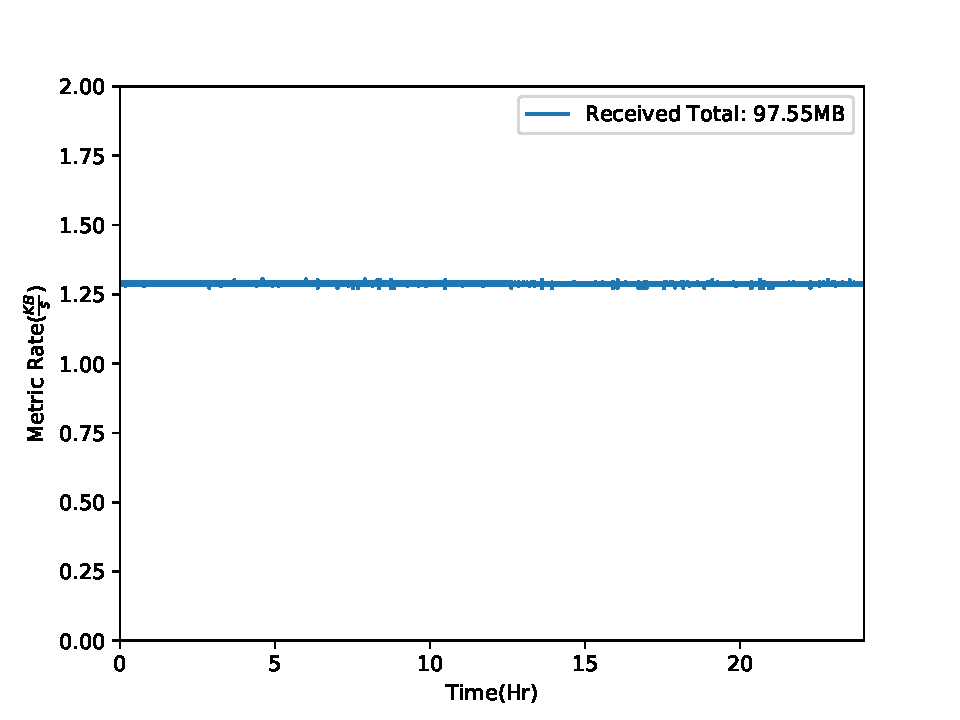
\includegraphics[width=1\linewidth]{img/napali_eval/napali_metric_bandwidth.pdf}
        \caption{}
        \label{expdes:fig:napali_metric_bandwidth}
    \end{subfigure}%
    \begin{subfigure}{.5\textwidth}
        \centering
        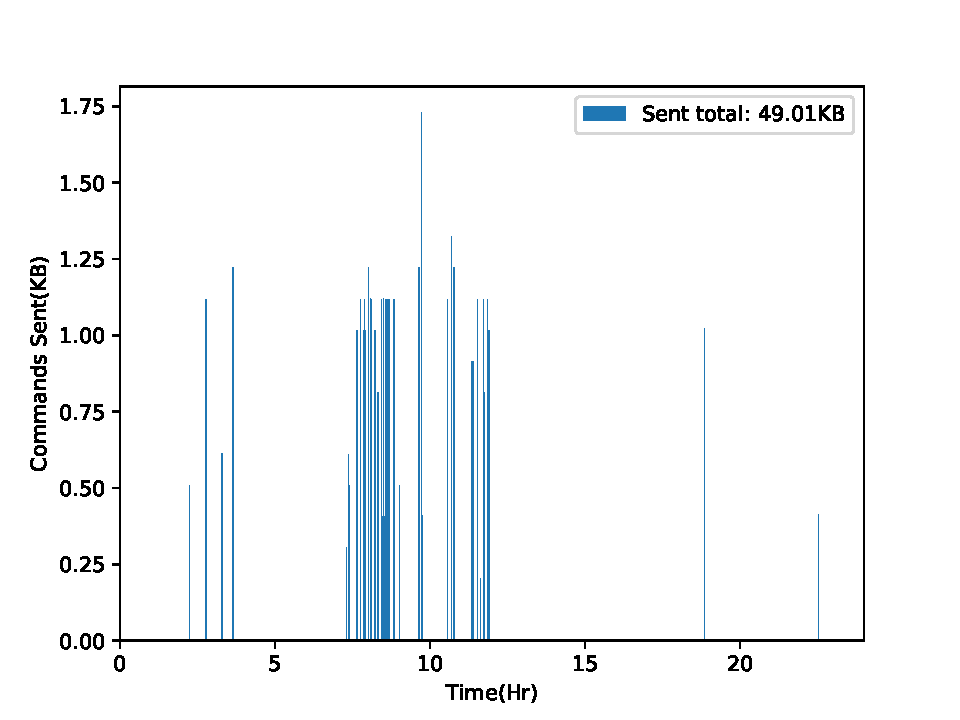
\includegraphics[width=1\linewidth]{img/napali_eval/napali_cmd_bandwidth.pdf}
        \caption{}
        \label{expdes:fig:napali_cmd_bandwidth}
    \end{subfigure}
    \caption{Penalties incurred by the Napali framework.
    a) Metrics received from 10 OPQ Boxes.
    b) Commands sent to 10 OPQ Box }
    \label{expdes:fig:napali_bandwidth_penalty}
\end{figure}

It should be noted that the Self-Triggered method does not incur the penalty of having to constantly transmit the device metrics to the sink, since all the event detection is performed on the device.
Figure \ref{expdes:fig:napali_metric_bandwidth} shows the amount of data received via metrics from 10 OPQ Boxes during the same 24 hours as the Figure \ref{expdes:fig:self_triggered_bandwidth}.
As expected the bandwidth requirement for metric transmission remains constant, since all OPQ Boxes send the metrics at fixed intervals.
While this penalty is significant as it constitutes 41\% of the total bandwidth used by Napali, the aggregate bandwidth is still shows a 440\% improvement over the Self-Triggered method.
Another penalty incurred by Napali is the two way communication requirement.
Each device which participated the event detection needed to receive a command with the temporal range which anomalous data.
Neither the Naive nor Self-Triggered methods require two-way communication, and as such there is no direct comparison to Napali.
Figure \ref{expdes:fig:napali_cmd_bandwidth} shows the command bandwidth consumption for 10 OPQ Boxes across 24 hours.
The total consumption was ~50kB, which is quite trivial for any modern sensor network.

During the 24 hours of shown in Figures \ref{expdes:fig:napali_bandwidth_penalty} and \ref{expdes:fig:self_triggered_bandwidth}, Napali captured 60 events, while the Self-Triggered method captured 878.
The average length of the Napali Event was 10s to the Self-Triggered 3s.
Of 60 Napali events, all 60 contained sub-threshold data.

Comparison of Napali with the Naive method was performed analytically.
Since the sampling rate of the OPQ Box is well characterized, and the number of OPQ Boxes is fixed, it is trivial to calculate the amount of raw data generated by the OPQ network during any time period.
In order to make this comparison fair, the raw data bandwidth will be scaled by the compression ratio of the state of the art compression algorithm specifically designed for power quality measurements.\cite{zhang2009new}
Operating at 12kSps, OPQ Box produces raw data at 24KB/s.
With state of the art compression operating at 90\% compression ratio and 5\% overhead of meta-data, one can expect a ~3KB/s stream of raw data for each OPQ box if it were to send the entirety of it to the sink.
For 10 OPQ Boxes we would expect the aggregate bandwidth of 30kB/s, and as such the bandwidth consumption 24.7GB/day.
During a 24 hour period, as shown in Figures \ref{expdes:fig:napali_bandwidth_penalty} and \ref{expdes:fig:self_triggered_bandwidth}, Napali used 234MB of bandwidth.
This corresponds to an over 100x improvement over the Naive method.

\begin{figure}[ht!]
    \centering
    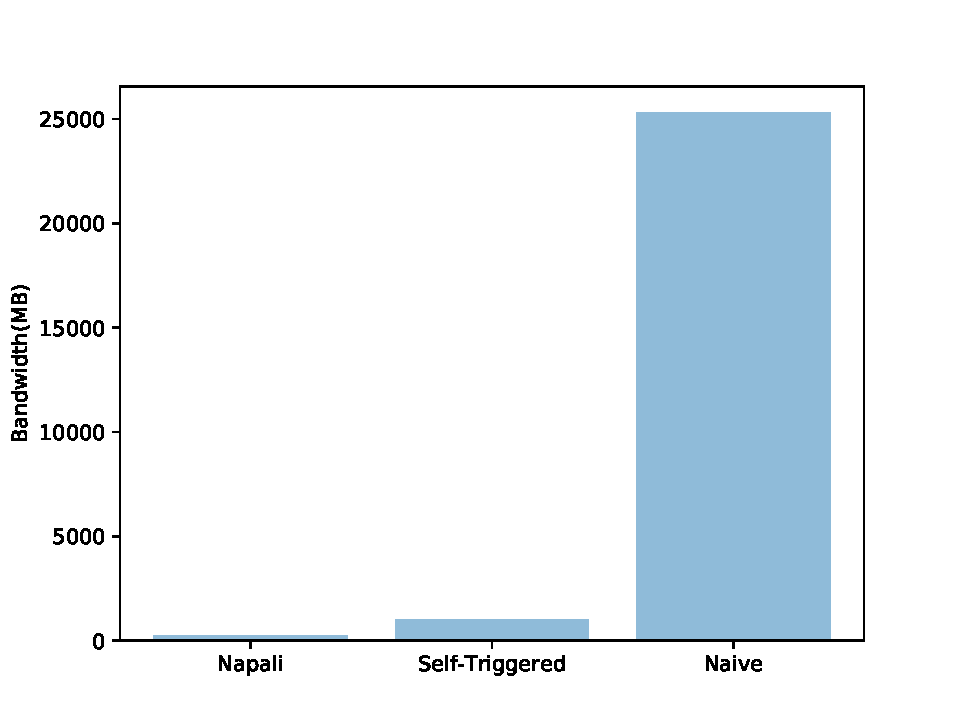
\includegraphics[width=0.8\linewidth]{img/napali_eval/napali_bandwidth_comparison.pdf}
    \caption{Bandwidth requirement comparison between three event detection methods.}
    \label{expdes:fig:bandwidth_master_comparison}
\end{figure}

Figure \ref{expdes:fig:bandwidth_master_comparison} shows the comparison between Napali as well as the Naive and Self-Triggered methods.
While Napali incurs additional costs described in Figure \ref{expdes:fig:napali_bandwidth_penalty} it outperforms the comparable methods.
Finally, the cost of the two way communication as shown in Figure \ref{expdes:fig:napali_cmd_bandwidth} is greatly outweighed by the bandwidth savings in the raw data reception.
Modern sensor networks greatly benefit from two way communication, as it allows on-demand health monitoring, and software updates.
With addition of Napali, two way communication allows for significant bandwidth requirement reduction in for the sensor network as a whole.

\subsection{Sink processing requirement under the Napali Framework}\label{subsec:sink-processing-requirement-under-the-napali-framework}
Sink processing requirements for event detection between Self-Triggered, Naive and Napali are quite different.
In general the processing requirement can be described as follows:
\begin{equation}\label{eq:detection_cost}
\begin{aligned}
    C_{total} = C_{metric\_extraction} + C_{detection}
\end{aligned}
\end{equation}

In the Equation \ref{eq:detection_cost} the $C_{total}$ is the total cost, $C_{metric\_extraction}$ is the cost of extracting metrics and $C_{detection}$ is the cost of event detection.\cite{de2015effective}
Each of the three methods, Napali, Self-Triggered, and Naive, has different sink costs associated with each parameter.

\subsubsection{Sink processing: Naive Method}

First, let's consider the Naive method.
In this case all of the metrics need to be extracted at the sink.
Disregarding the processing power required to keep up with the data rate described in Section \ref{subsec:napali-bandwidth-usage} the $C_{feature\_extraction}$ can be measured empirically.
In order perform this measurement, OPQ Box software was built for an x86 architecture and stress-tested.
Instead of acquiring data from a device driver, the feature extraction stack was supplied with synthetic data.
Finally, the ZMQ communication was removed and replaced with the performance analysis code.
Stress test was performed on a Intel Core i9-8950HK CPU with thermal management disabled running at 2.9GHz.
Under such conditions, the metric extraction stack was able to extract features from 1s worth of raw data in $800us$ running on a single core.
Since metric extraction has no inter-device data dependencies, a modern 8 core CPU can expect to keep up with feature extraction from 1000 devices.
If an OPQ Box sensor is used with 16 bit samples and 12kSps ADC, aggregate bandwidth for such system is 10.8Gbps, which is well within the realm of a collocated server with dual 10Gbps network interfaces.
$C_{detection}$ cost can be made linear with the number of devices.
If a rolling window is applied to metrics as they are generated, raw data from all devices contained in the window with an offending threshold metric can be retained for later analysis.
While simple, this method will collect all of the gridwide events along with a large number of false positives.
In synthetic benchmarks, the $C_{detection}$ made up less then $0.01\%$ of the computational cost when compared to $C_{feature\_extraction}$
and does not significantly contribute to the $C_{total}$.

\subsubsection{Sink Processing: Naive Method}

In contrast to the Naive method, the Self-Triggered method, has no sink processing requirements, since all of the feature-extraction is performed on the edge device.
Thus, Self-Triggered method event detection is only limited by the available network bandwidth.

\subsubsection{Sink Processing: Napali Method}

Napali, being a hybrid of Naive and Self-Triggered methods, moves the $C_{metric\_extraction}$ cost to the edge devices, while retaining
the $C_{detection}$ at the sink.
Unlike the Naive case, napali performs additional computations on the features in order to detect sub-threshold events while excluding the local noise.
However, even with additional metric analysis the Napali stack was able to process synthetic data from 100000 devices on a single core of an a Intel Core i9-8950HK CPU.
This would allow a single server running Makai to provide 50\% coverage of households in the city of Honolulu.

\subsubsection{Sink Processing: Event Classification}

The final step of any power quality analysis stack is event classification.
Every event collected by an event detection system must be analyzed and classified according to their severity and type.
While Makai/Napali are not responsible for event classification it is important to consider the event classification cost when discussing sink processing requirements.
In the case of the Naive method, events which are detected are a mix of local and global events.
However, every event will contain a waveform from every device on the network.
For the Self-Triggered method, only the events which cross the threshold will be considered for classification.
While Self-Triggered events will not contain false positives and sub-threshold events, vast majority of acquired waveforms are comprised of local disturbances.
Finally, Napali produces high quality events which only contain high fidelity sub and over threshold events, while ignoring local disturbances.
During the campus deployment Napali detected 302 Events comprised of 1561 individual device waveforms a week on average.
The Self-Triggered method detected 26520 offending waveforms.
If we assume unitary classification cost, classification computational requirements for one week of data are shown in Figure \ref{expdes:fig:classification}.
\begin{figure}[ht!]
    \centering
    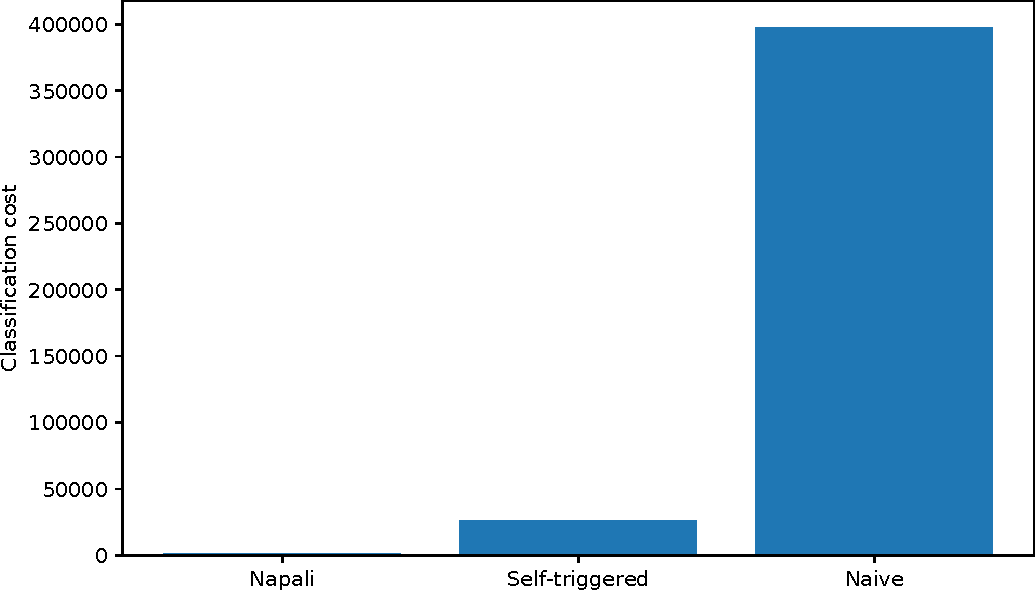
\includegraphics[width=0.8\linewidth]{img/napali_eval/classification_cost.pdf}
    \caption{Classification cost based on the expected amount of waveforms for the three considered methods.}
    \label{expdes:fig:classification}
\end{figure}


\subsection{Effects of latency in the Napali framework}\label{subsec:effects-of-latency-in-the-napali-framework}

In order to understand the effects of latency on Makai in the OPQ deployment, we examined the event length and round trip latency for OPQ Boxes.
These parameters are shown in Figure \ref{expdes:fig:el_la}.

\begin{figure}[ht!]
    \centering
    \begin{subfigure}{.45\textwidth}
        \centering
        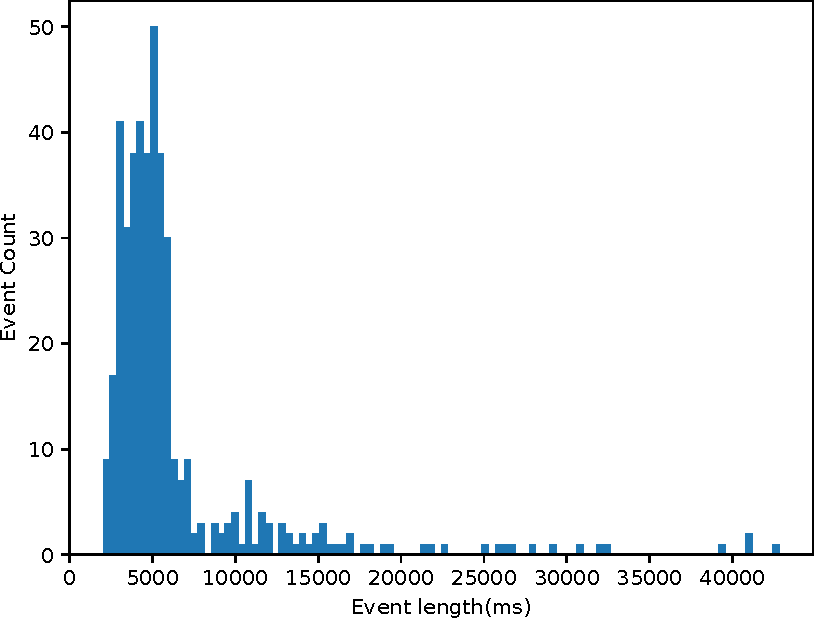
\includegraphics[width=1\linewidth]{img/napali_eval/event_length.pdf}
        \caption{}
        \label{expdes:fig:event_length}
    \end{subfigure}\hspace{5mm}
    \begin{subfigure}{.45\textwidth}
        \centering
        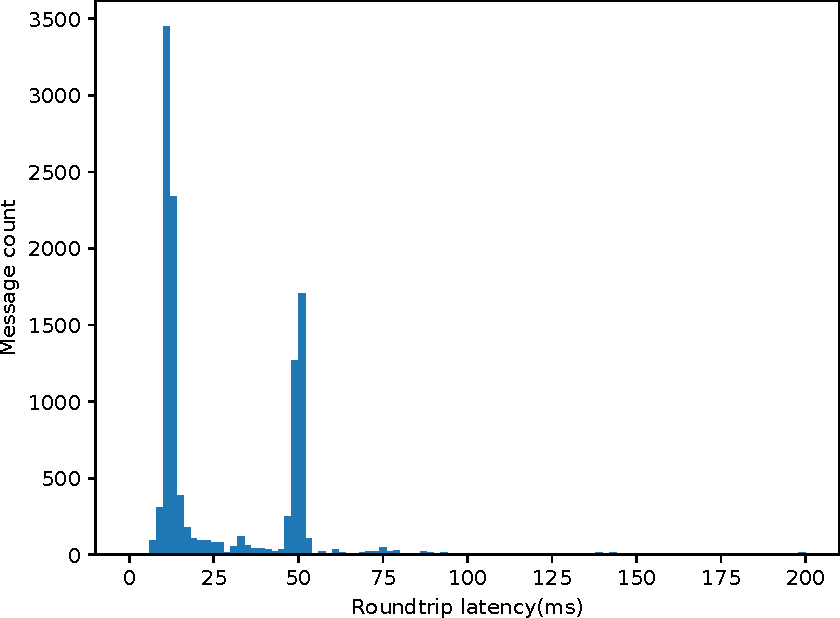
\includegraphics[width=1\linewidth]{img/napali_eval/latency.pdf}
        \caption{}
        \label{expdes:fig:latency}
    \end{subfigure}
    \caption{Event length(a) and message latency(b) observed by the OPQ devices.}

    \label{expdes:fig:el_la}
\end{figure}

Figure \ref{expdes:fig:event_length} was generated from 1000 events or about a month of data.
As depicted, the majority of events captured by napali were less then 20s in length, with a few stragglers hitting a 40sec mark.

Figure \ref{expdes:fig:latency} was generated by requesting a 20s event from all OPQ Box devices and timing the amount of time it takes them to respond.
Since this measurement can be performed synthetically without waiting for an anomaly, 10000 samples were used, which equates to approximately ten months of real world measurements.
Latencies clustered into two groups, likely based on the signal strength of the WIFI networks, with means of 12.5ms and 50ms.
A few stragglers were observed at at 200ms and a single device had a latency of 1.2s, and was omitted from Figure \ref{expdes:fig:latency} for clarity.

Since OPQ Boxes communicate via wifi it is common for them to loose connections to the access point, and reconnect some time later.
This behaviour can be quantified in the OPQ network by examining the trend dataset.
Trends are generated for each device at 1 minute intervals.
By comparing the database insertion time and the timestamp reported by the device, it is possible to find trends which were delayed in transit.
Out of two months of data only 73 delayed trends were reported, and are shown in Figure \ref{expdes:fig:trend_latency}.
While the majority of trends were delayed by less then 60 seconds, one was delayed by 3 minutes.

OPQ Box does not utilize compression in the RDRB.
The maximum safe size of RDRB was found to be 100MB of 256MB of total system memory.
This way there is enough memory left over on the device to prepare the data for transmission in the diabolical case where Makai requests the entire buffer.
Given that the sampling rate and data size is fixed, 100MB of RDRB can store about 1.1 hours of raw waveform.
As evident from Figure \ref{expdes:fig:el_la} under normal operating conditions, even with degraded latency, no event will overrun the RDRB.
Even with the longest observed event/worst observed latency, the maximum delay is on the order of 50s, or slightly longer then 1\% of the maximum tolerated latency.
Under abnormal conditions, such as a WIFI drop, the maximum delay may be on the order of 5 minnutes, which is on the order of 8\% of maximum tolerated latency.

\begin{figure}[ht!]
    \centering
    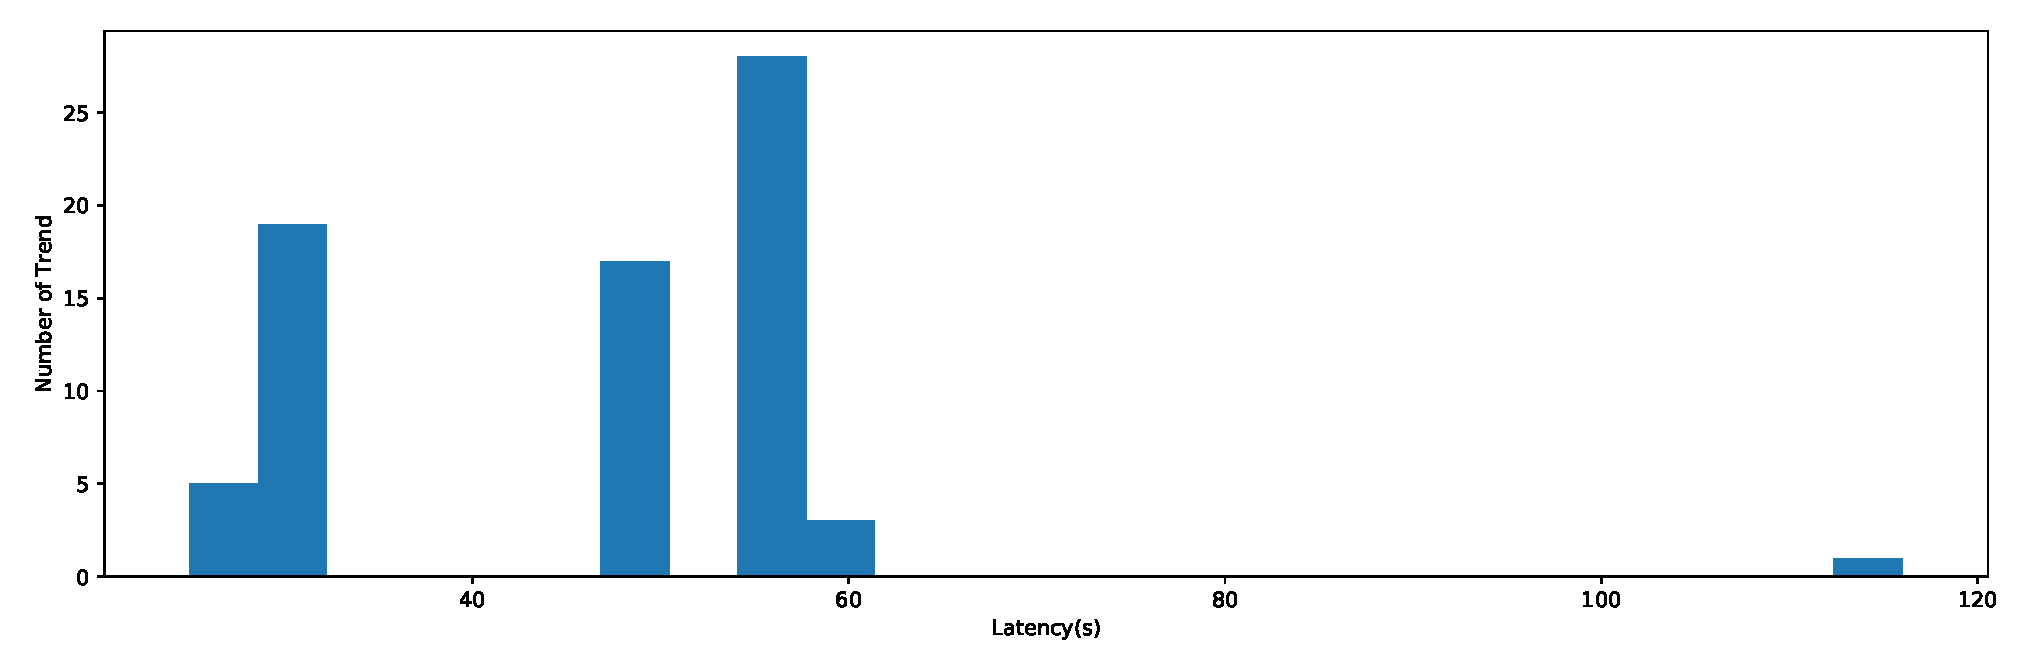
\includegraphics[width=1\linewidth]{img/napali_eval/trend_latency.pdf}
    \caption{Delay in trend creation, indicating a network failure.}
    \label{expdes:fig:trend_latency}
\end{figure}


Device latency has a different effect on Napali, Naive and Self-Triggered methods.
The Self-Triggered method is completely unaffected by latency, since event detection is performed entirely on the device.
The Naive method is affected the most, since the sink performs all of the event detection computations.
In this case if latency is asymmetric across the devices, and the device with the highest latency observes an over-threshold condition,
there is potential for waveforms from the rest of the network to get falsely discarded.
Napali only requires metrics for anomaly detection, and as such, the sink does not need to buffer raw data in anticipation of a potential event.

The Naive method must buffer enough raw data to be able to handle network failures and interruptions.
If a device with an over the threshold metric is delayed, the Naive method must keep raw waveforms for all devices in order to store them for later analysis.
In the case of OPQ, as described in Figures \ref{expdes:fig:trend_latency} and \ref{expdes:fig:el_la} the maximum observed latency may be on the order of 5 minutes.
This implies, for each device Naive method must buffer $~$7MB of raw waveform per device.
In reality, for large deployment both the rate of network failre and latency is expected to be higher then those reported on the UH network.

In the case of Napali only the metrics need to be buffered for event detection.
An optimal amount of metrics storage is determined by the worst case latency and the maximum expected event size
However, since the overhead of buffering metrics is so small there is no reason to not maintain a measurement buffer appropriate to accumulate the maximum delay that the OPQ Box can tolerate.
This limit is governed by the amount of data that the RDRB can store, thus even if an over the threshold metrics are transmitted the delay slightly less then the RDRB capacity, Napali will still acquire the raw waveform.
The amount of memory required for each device can be derived by analysing the metric size and the frequency of metric transmission.
In the case of OPQ each measurement is 24bytes in size and they are transmitted at 1 measurement per second resulting in the total memory consumption of 84kB for 1 hour of metric storage.
A modest server can support Napali/Makai with 100000 devices while utilising 8GB of memory for 1 hour of metric storage, a 100 times improvement over the Naive method only buffering 5 minutes of raw waveforms.


\subsection{Summary of Computational and Network Resource Utilisation}\label{subsec:summary-of-computational-and-network-recource-utilisaztion}

Sections \ref{subsec:napali-bandwidth-usage}, \ref{subsec:sink-processing-requirement-under-the-napali-framework} and \ref{subsec:effects-of-latency-in-the-napali-framework} describe the computational utility of the Napali framework, when compared to the Naive and Self-Triggered methods.
Using the insights described above we can compare the number of devices that the three methods in question can support on a modest collocated server.
Our hypothetical server is a 4 core machine, with each core equivalent to an Intel i9-8950HK we have been using for benchmarking.
It is further equipped with 8GB of random access memory and a single symmetric 1Gb uplink to OPQ devices.
For comparison we consider the three metrics described above: bandwidth, computational cost and memory utilization.
When comparing network computational cost, the classification cost is not considered, since these results illustrate the cost of the event detection only.
Notice, that we use linear scaling for Napali event rate.
Napali uses a statistical approach, in order to locate subthreshold events.
Intuitively, this statistical approach would not scale linearly, since as the number of devices in the network increases, the probability of multiple devices observing unrelated
subthreshold event increases as well.
However this can be mitigated using device clustering as shown in Section \ref{subsec:event-clustering-evaluation}, which results in linear scalability.
\begin{center}
    \begin{table}[!ht]
        \caption{Method comparison for a typical collocated server: Bandwidth}
        \label{tbl:expdes:bandwidth}
        \begin{tabularx}{\textwidth}[t]{sssb}
             &\textbf{Napali} &\textbf{Self-Triggered} &\textbf{Naive}  \\
            \arrayrulecolor{black}\hline
            \textbf{\# of devices} &44000 & 10000 & 800\\
            \arrayrulecolor{black}\hline
        \end{tabularx}
    \end{table}
\end{center}

Table \ref{tbl:expdes:bandwidth} describes the bandwidth limitation across the three methods, assuming no overhead and 100\% utilization on the 1Gb link.
Napali is a clear winner in this case, since it is able to to support significantly more devices before becoming bandwidth limited.

\begin{center}
    \begin{table}[!ht]
        \caption{Method comparison for a typical collocated server: CPU}
        \label{tbl:expdes:cpu}
        \begin{tabularx}{\textwidth}[t]{sssb}
            &\textbf{Napali} &\textbf{Self-Triggered} &\textbf{Naive}  \\
            \arrayrulecolor{black}\hline
            \textbf{\# of devices} &400000 & $\infty$ & 1000\\
            \arrayrulecolor{black}\hline
        \end{tabularx}
    \end{table}
\end{center}

Table \ref{tbl:expdes:cpu} describes the CPU limitation across three methods, assuming 100\% CPU utilization on all 4 cores.
In the Self-Triggered method, event detection is performed entirely on the device, so it incurs no CPU cost.
However, the cost of event detection with Napali is so low, that it hardly affects it's utility.
Naive method fairs the worst between the three since it relegates all of the event detection cost to the sink.

\begin{center}
    \begin{table}[!ht]
        \caption{Method comparison for a typical collocated server: Memory}
        \label{tbl:expdes:memory}
        \begin{tabularx}{\textwidth}[t]{sssb}
            &\textbf{Napali} &\textbf{Self-Triggered} &\textbf{Naive}  \\
            \arrayrulecolor{black}\hline
            \textbf{\# of devices} &100000 & $\infty$ & 1000\\
            \arrayrulecolor{black}\hline
        \end{tabularx}
    \end{table}
\end{center}

Table \ref{tbl:expdes:memory} describes the memory limitations across the three methods, assuming 100\% memory utilization.
Again, with no sink requirements, the Self-Triggered method requires no memory buffer for event detection.
Napali buffers 1Hr of metrics in order to accommodate on devices with excessive latency and handle network faults.
Naive method must maintain a buffer of raw waveforms on the sink, which leads to a memory bottleneck while only maintaining a 5 minute buffer.

\begin{center}
    \begin{table}[!ht]
        \caption{Method comparison for a typical collocated server: Worst of all metrics}
        \label{tbl:expdes:final_utilisation}
        \begin{tabularx}{\textwidth}[t]{sssb}
            &\textbf{Napali} &\textbf{Self-Triggered} &\textbf{Naive}  \\
            \arrayrulecolor{black}\hline
            \textbf{\# of devices} &44000 & 10000 & 800\\
            \arrayrulecolor{black}\hline
        \end{tabularx}
    \end{table}
\end{center}

Table \ref{tbl:expdes:final_utilisation} describes the final tally across the three methods.
It illustrates how many devices our hypothetical collocated server can handle before becoming limited in one of three metrics.
All three methods are limited by the bandwidth, however, even with additional bandwidth the Naive method would quickly run out of computational resources to keep up with the data stream.
As such, when it comes to efficiency of gridwide monitoring Napali is a clear winner suitable for deployment across a large portion of grid endpoints.
Self-Triggered method is close second, but as we will see in the next two sections, it performes poorly when it comes to detection efficiency.
Finally, Naive method is the most computationally expensive at the sink.
However, it is also the most robust when it comes to event detection, both local, gridwide, and subthreshold.
As such, the Naive method is best left for monitoring high value infrastructure such as substations and production centers which can afford the additional computational and bandwidth cost.

\subsection{Temporal locality triggering of the Napali framework} \label{subsec:temporal-locality-triggering-of-the-napali-framework}
As mentioned previously, during the University of Hawaii deployment the OPQ network worked along side the utility grade meters embedded in the University power delivery infrastructure.
Data from these devices provided ground truth when it came to evaluating OPQ power quality anomaly detection.
Before we delve deeper into that, will compare the OPQ Box and utility meter metric extraction capabilities.

\subsubsection{Utility meter metric extraction comparison} \label{subsubsec:utility-box-comp}
8 OPQ devices were collocated along with smart utility meters capable of logging power quality metrics.
This analysis focuses on Device 1000 along with a smart utility meter labeled POST\_MAIN\_2 which is located upstream of Device 1000.
POST\_MAIN\_2 is monitoring a 480V line going into the Pacific Ocean and Science Building prior to it's conditioning and stepped down into the domestic 120V.

\paragraph{Frequency:}
A plot of 1 week of frequency measurements collected by the OPQ Box 1000 and POST\_MAIN\_2 is shown in Figure \ref{expdes:fig:postmain2:freq}.

\begin{figure}[ht!]
    \centering
    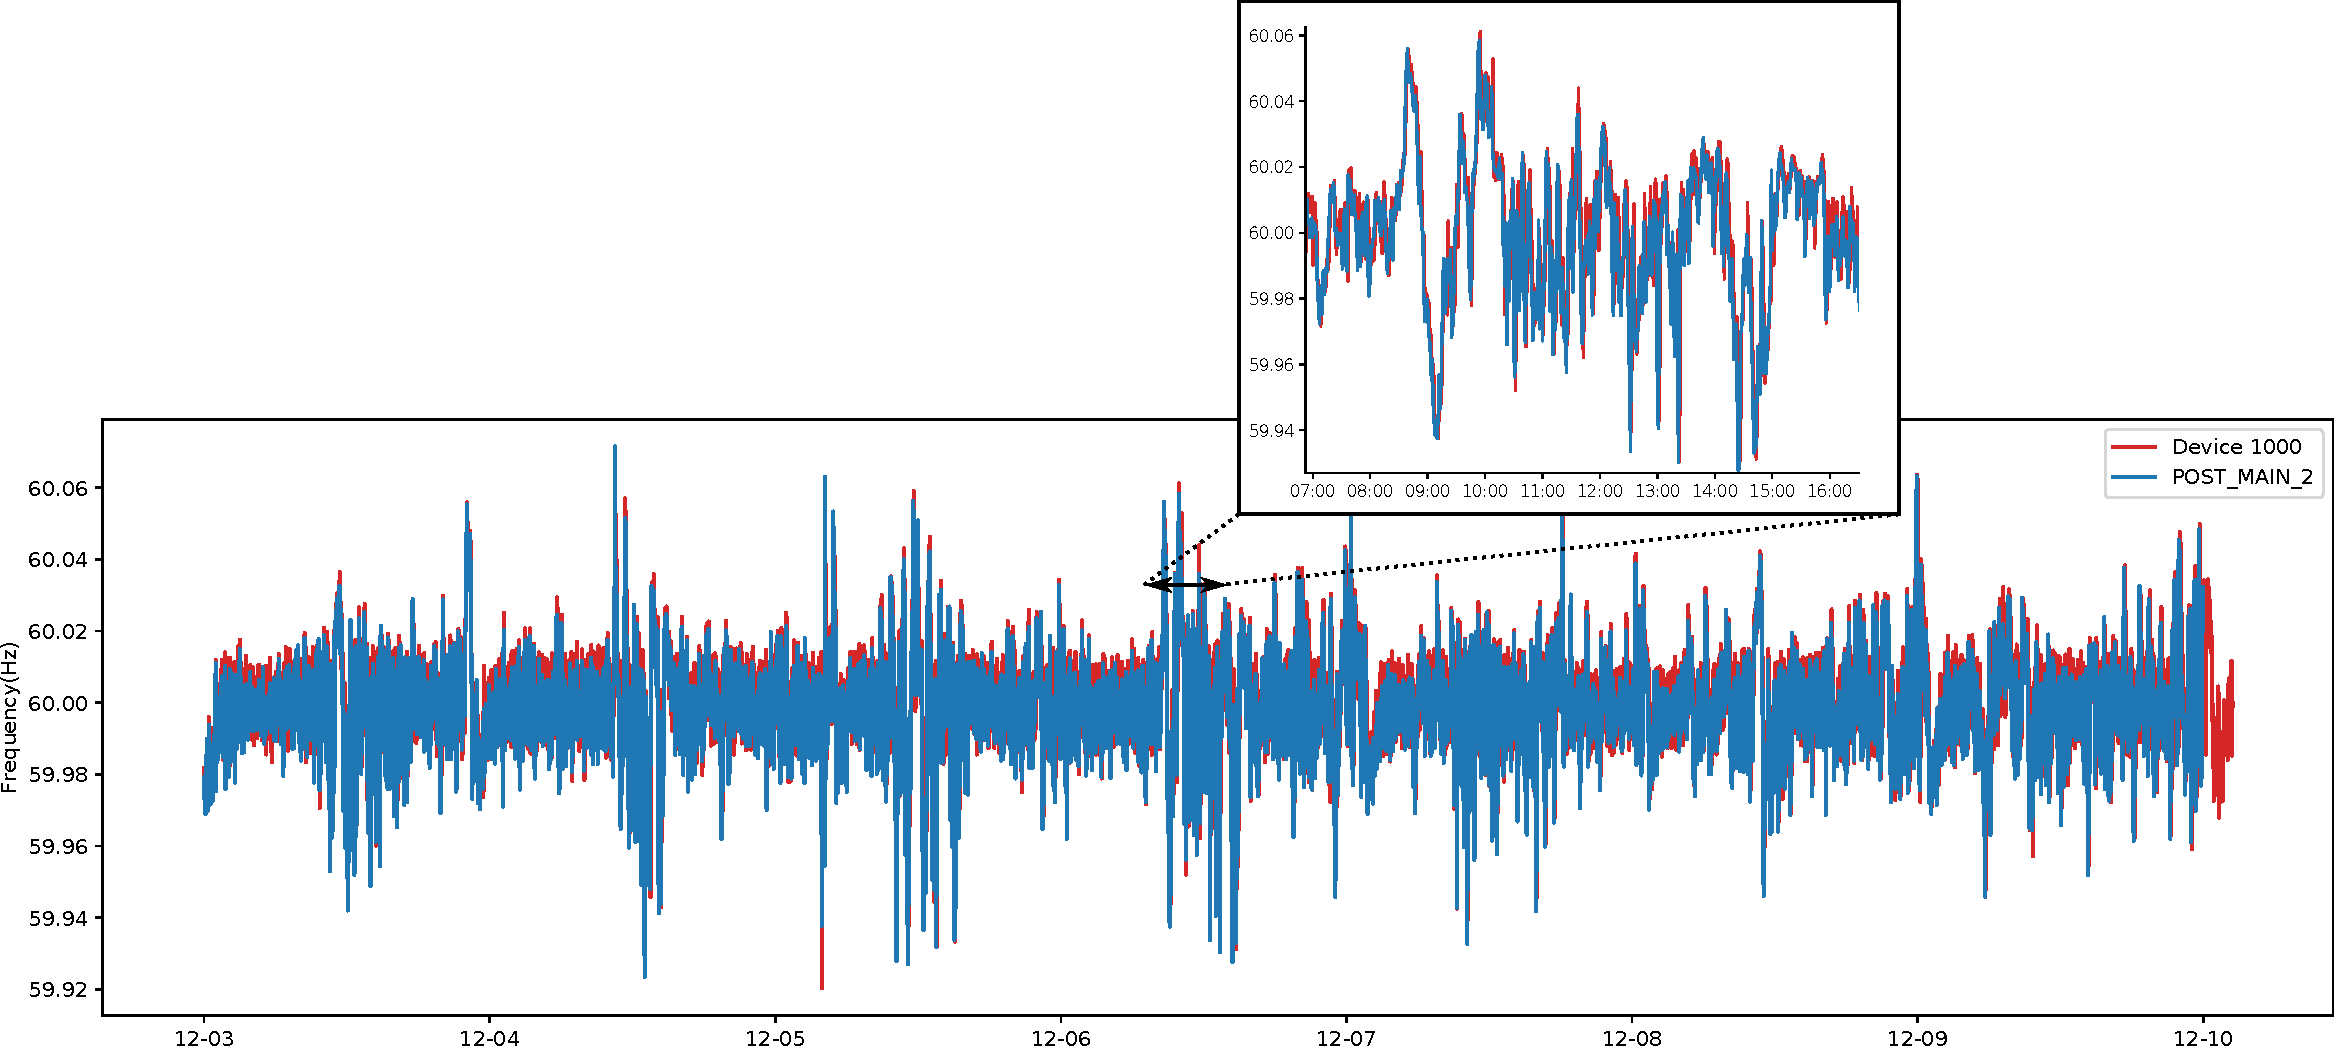
\includegraphics[width=1\linewidth]{img/napali_eval/gt/gt_frequency.pdf}
    \caption{Frequency metric for the POST\_MAIN\_2 utility meter and OPQ Box 1000.}
    \label{expdes:fig:postmain2:freq}
\end{figure}

OPQ Box and the utility meter track the fundamental frequency across all devices throughout the entire deployment.
This is expected since the fundamental frequency must be stable across the entire grid in order for it to operate properly
This parity is further demonstrated in Figure \ref{expdes:fig:postmain2:freq_diff} where the frequency recorded by the two devices was subtracted from one another.
These differences were histogramed and statistically analyzed.

\begin{figure}[ht!]
    \centering
    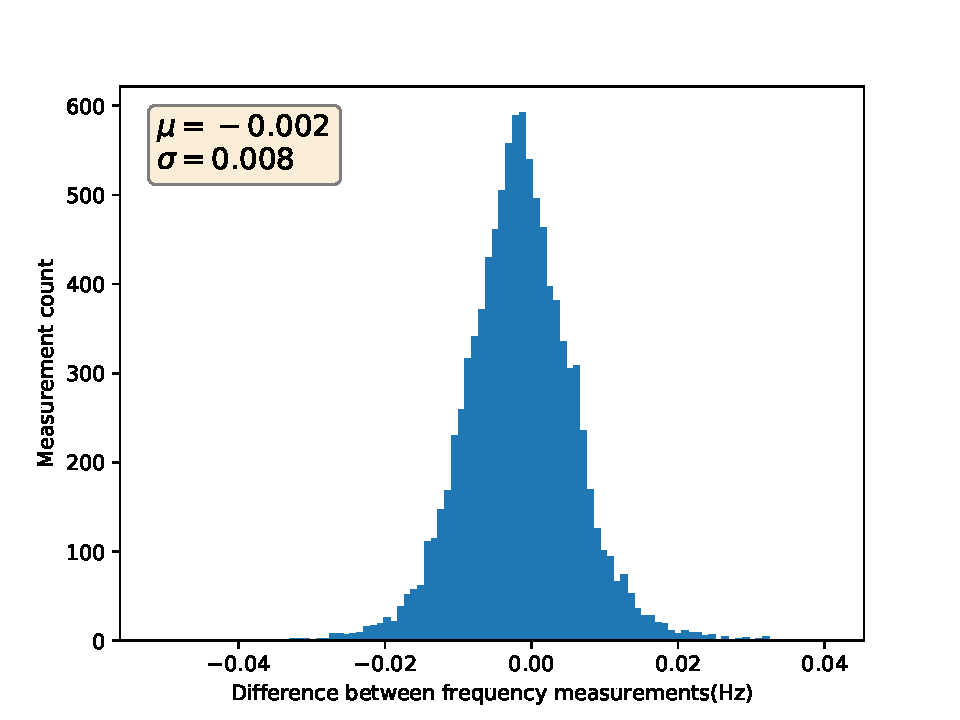
\includegraphics[width=0.6\linewidth]{img/napali_eval/gt/gt_f_diff.pdf}
    \caption{Difference in the frequency metric between POST\_MAIN\_2 utility meter and OPQ Box 1000.}
    \label{expdes:fig:postmain2:freq_diff}
\end{figure}

Synthetic benchmarks showed the OPQBox frequency measurement capability on the order of 200x better then the error reported in Figure \ref{expdes:fig:postmain2:freq_diff}.
This is likely due to the fact that both comparisons are done over 1 minute averages of frequency, and the offset of where the minute average starts is not well described in the utility data.
Regardless, with the power quality threshold of $0.1Hz$ an error of two devices with $\sigma=8mHz$ is perfectly acceptable to draw our conclusions regarding the Napali temporal trigger efficiency.

\paragraph{THD:}
A plot of 1 week of THD measurements collected by the OPQ Box 1000 and POST\_MAIN\_2 is shown in Figure \ref{expdes:fig:postmain2:thd}.

\begin{figure}[ht!]
    \centering
    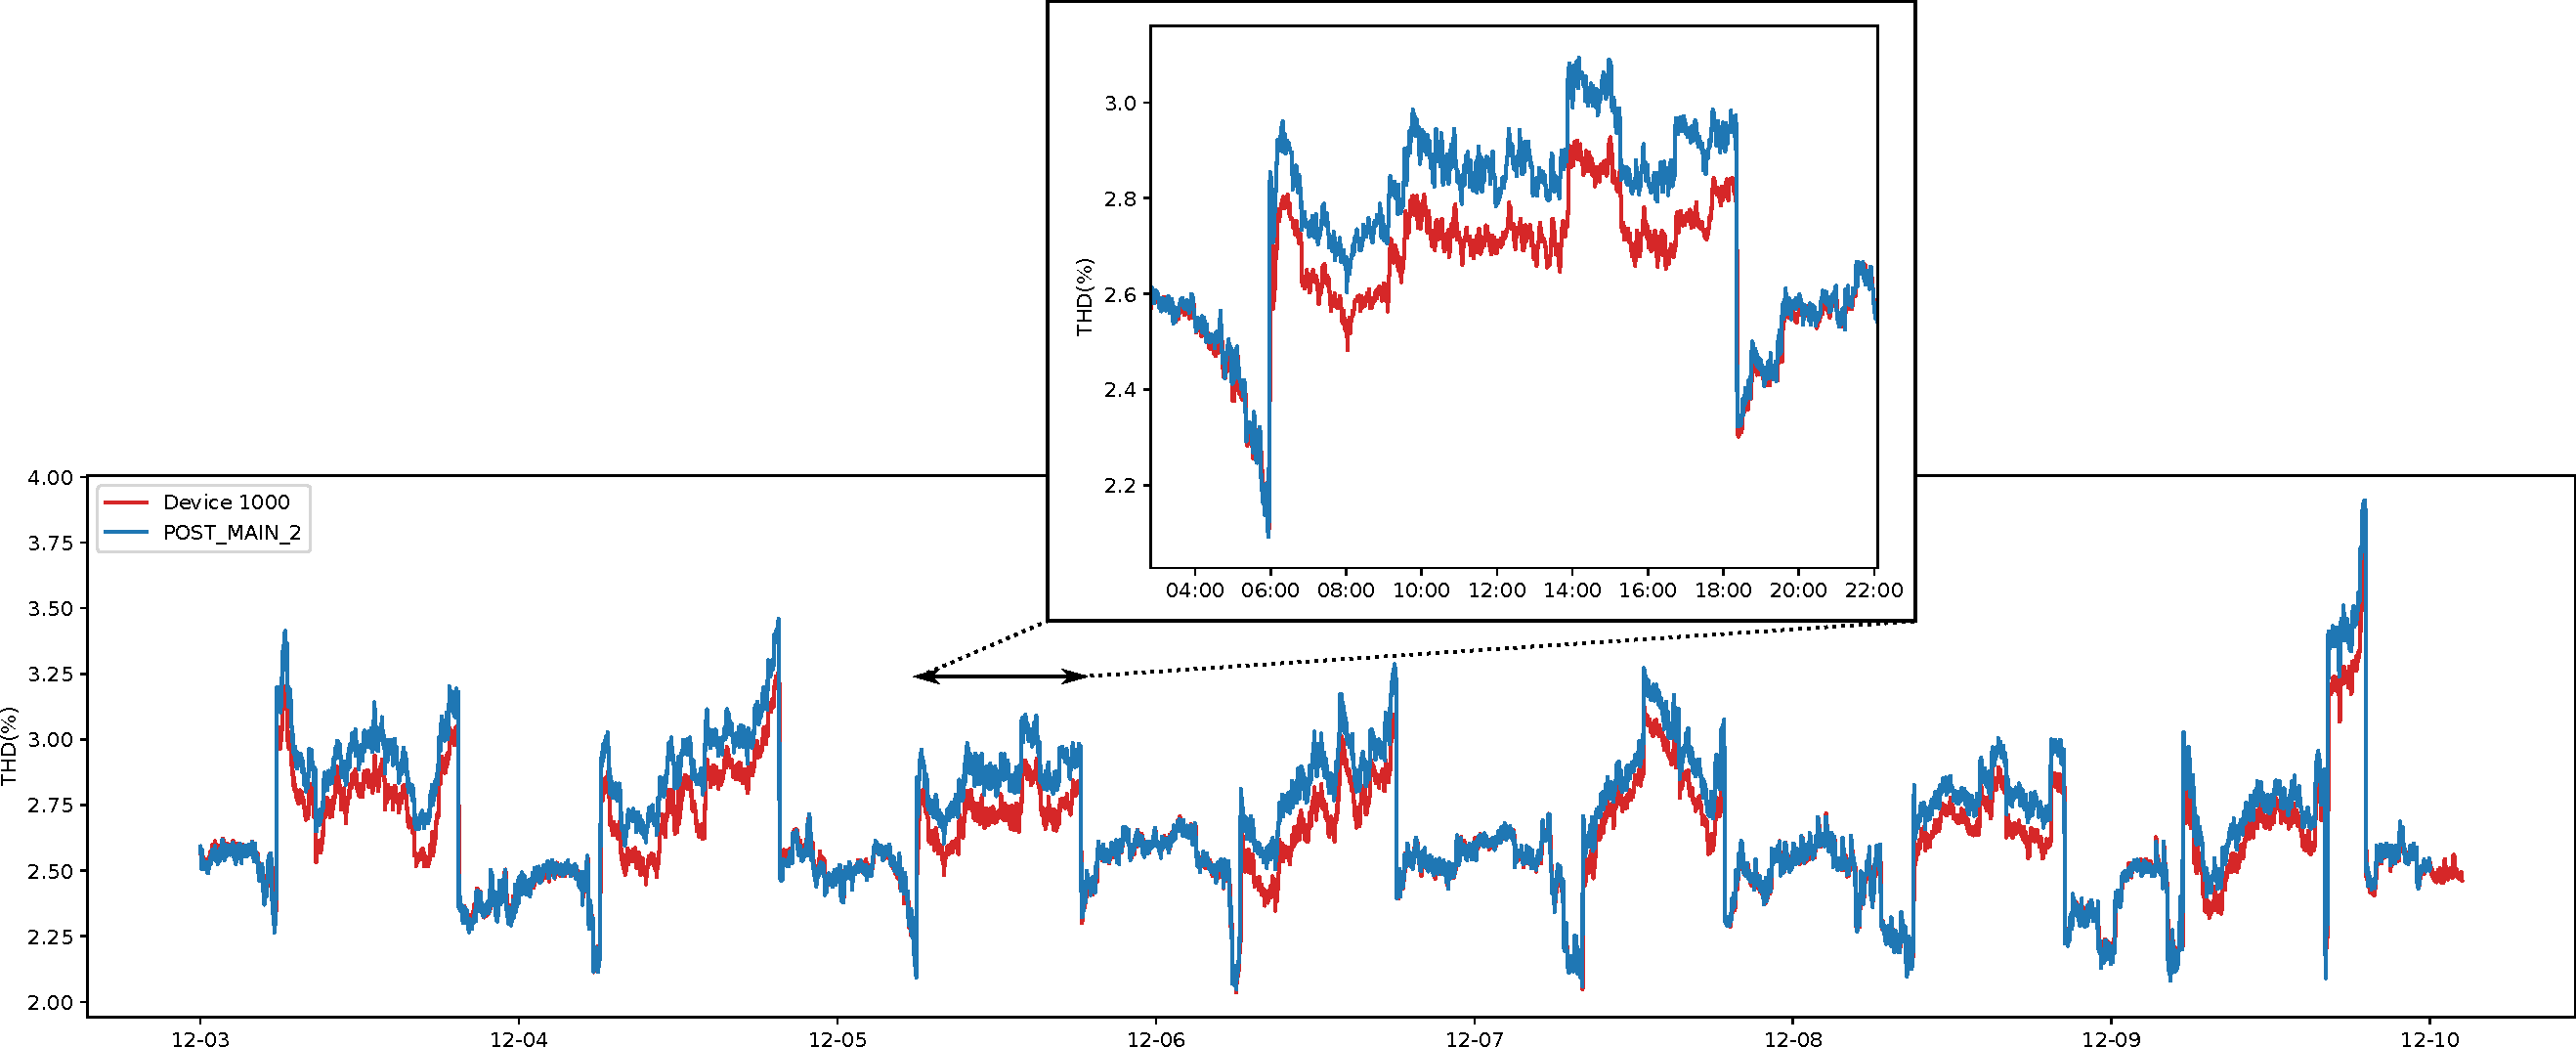
\includegraphics[width=1\linewidth]{img/napali_eval/gt/gt_thd.pdf}
    \caption{THD metric for the POST\_MAIN\_2 utility meter and OPQ Box 1000.}
    \label{expdes:fig:postmain2:thd}
\end{figure}

Unlike the frequency measurements, THD shows anomalous behaviour during the daylight hours.
Particularly, form 6:00-18:00 daily the THD measurement diverges by a fraction of a percent between the devices.
Since the POST\_MAIN\_2 meter is located upstream of Device 1000 on the power grid hierarchy, there is likely a reactive power compensation or a THD filter system positioned between the two devices.
The fact thea the minute differences in THD are tracked equally well, albeit with an aforementioned offset is particularly interesting.
This fact is further illustrated in Figure \ref{expdes:fig:postmain2:thd_diff}.

\begin{figure}[ht!]
    \centering
    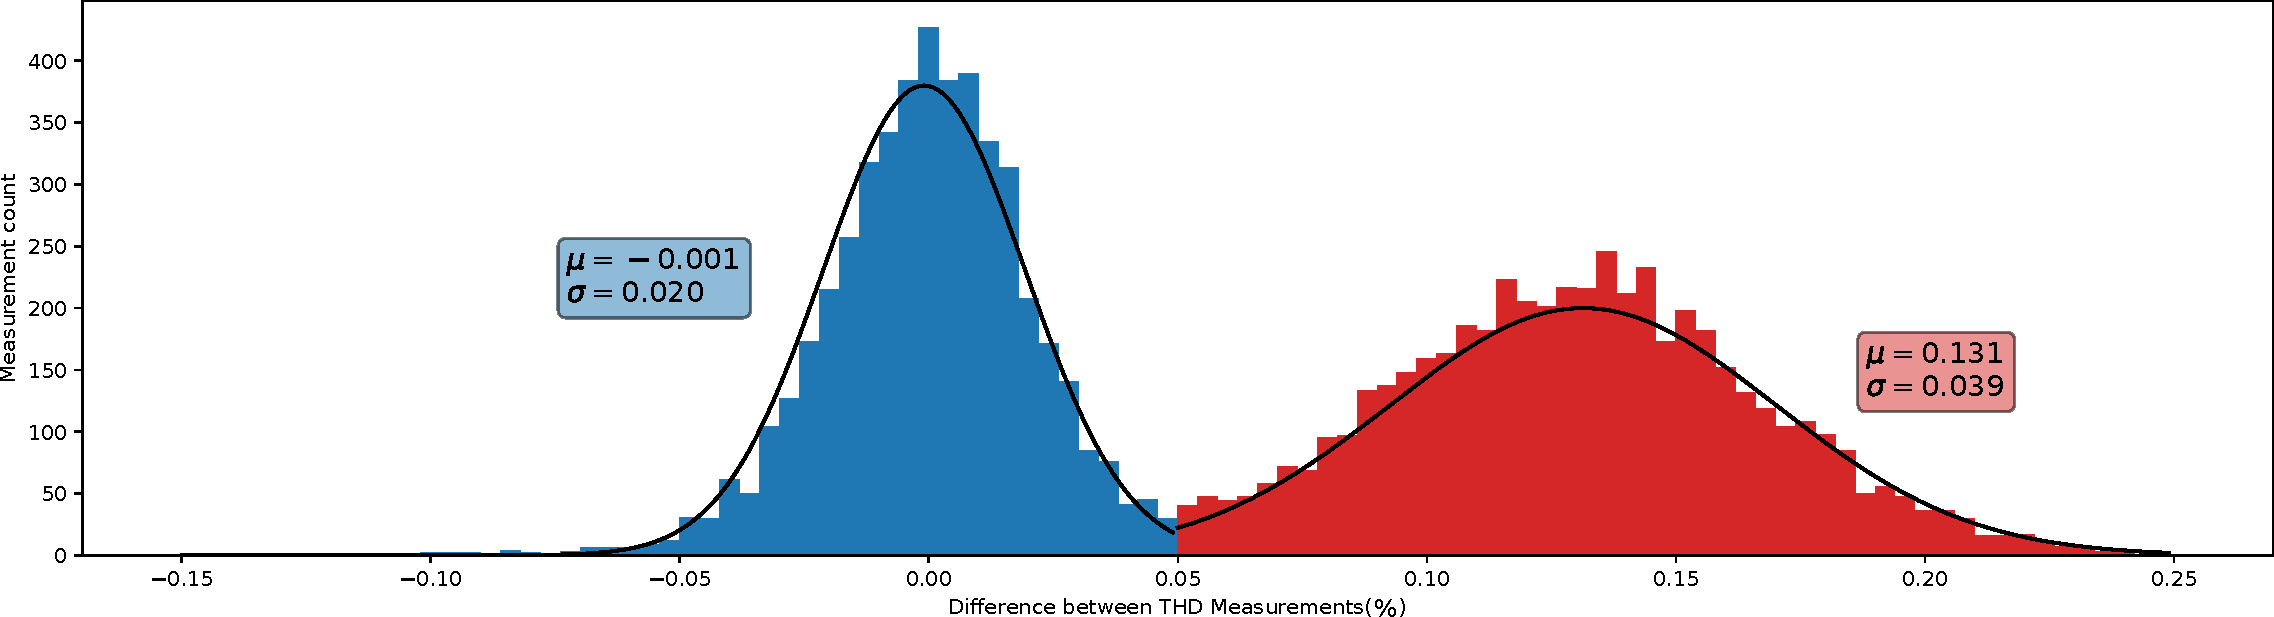
\includegraphics[width=1\linewidth]{img/napali_eval/gt/gt_thd_diff.pdf}
    \caption{Difference in the THD metric between POST\_MAIN\_2 utility meter and OPQ Box 1000.}
    \label{expdes:fig:postmain2:thd_diff}
\end{figure}

Figure \ref{expdes:fig:postmain2:thd_diff} shows the difference in measurement between the OPQ device and the utility meter.
In blue are the samples occurring during the seemingly coincidental regions of 18:00-6:00.
these regions are characterized by an excellent agreement between the two devices, with difference given by $sigma =0.02\%$.
This level of agreement is comparable to the synthetic benchmarks of the OPQ box with a well calibrated source.
The red region is the anomalous region, where the two sets of measurements are offset by the $\mu = 0.13\%$.
Even though the accuracy suffered, measurement remained precise down to $\sigma=0.04\%$.

\paragraph{RMS Voltage:}
A plot of 1 week of \underline{normalized} voltage measurements collected by the OPQ Box 1000 and POST\_MAIN\_2 meter is shown in Figure \ref{expdes:fig:postmain2:rms}.

\begin{figure}[ht!]
    \centering
    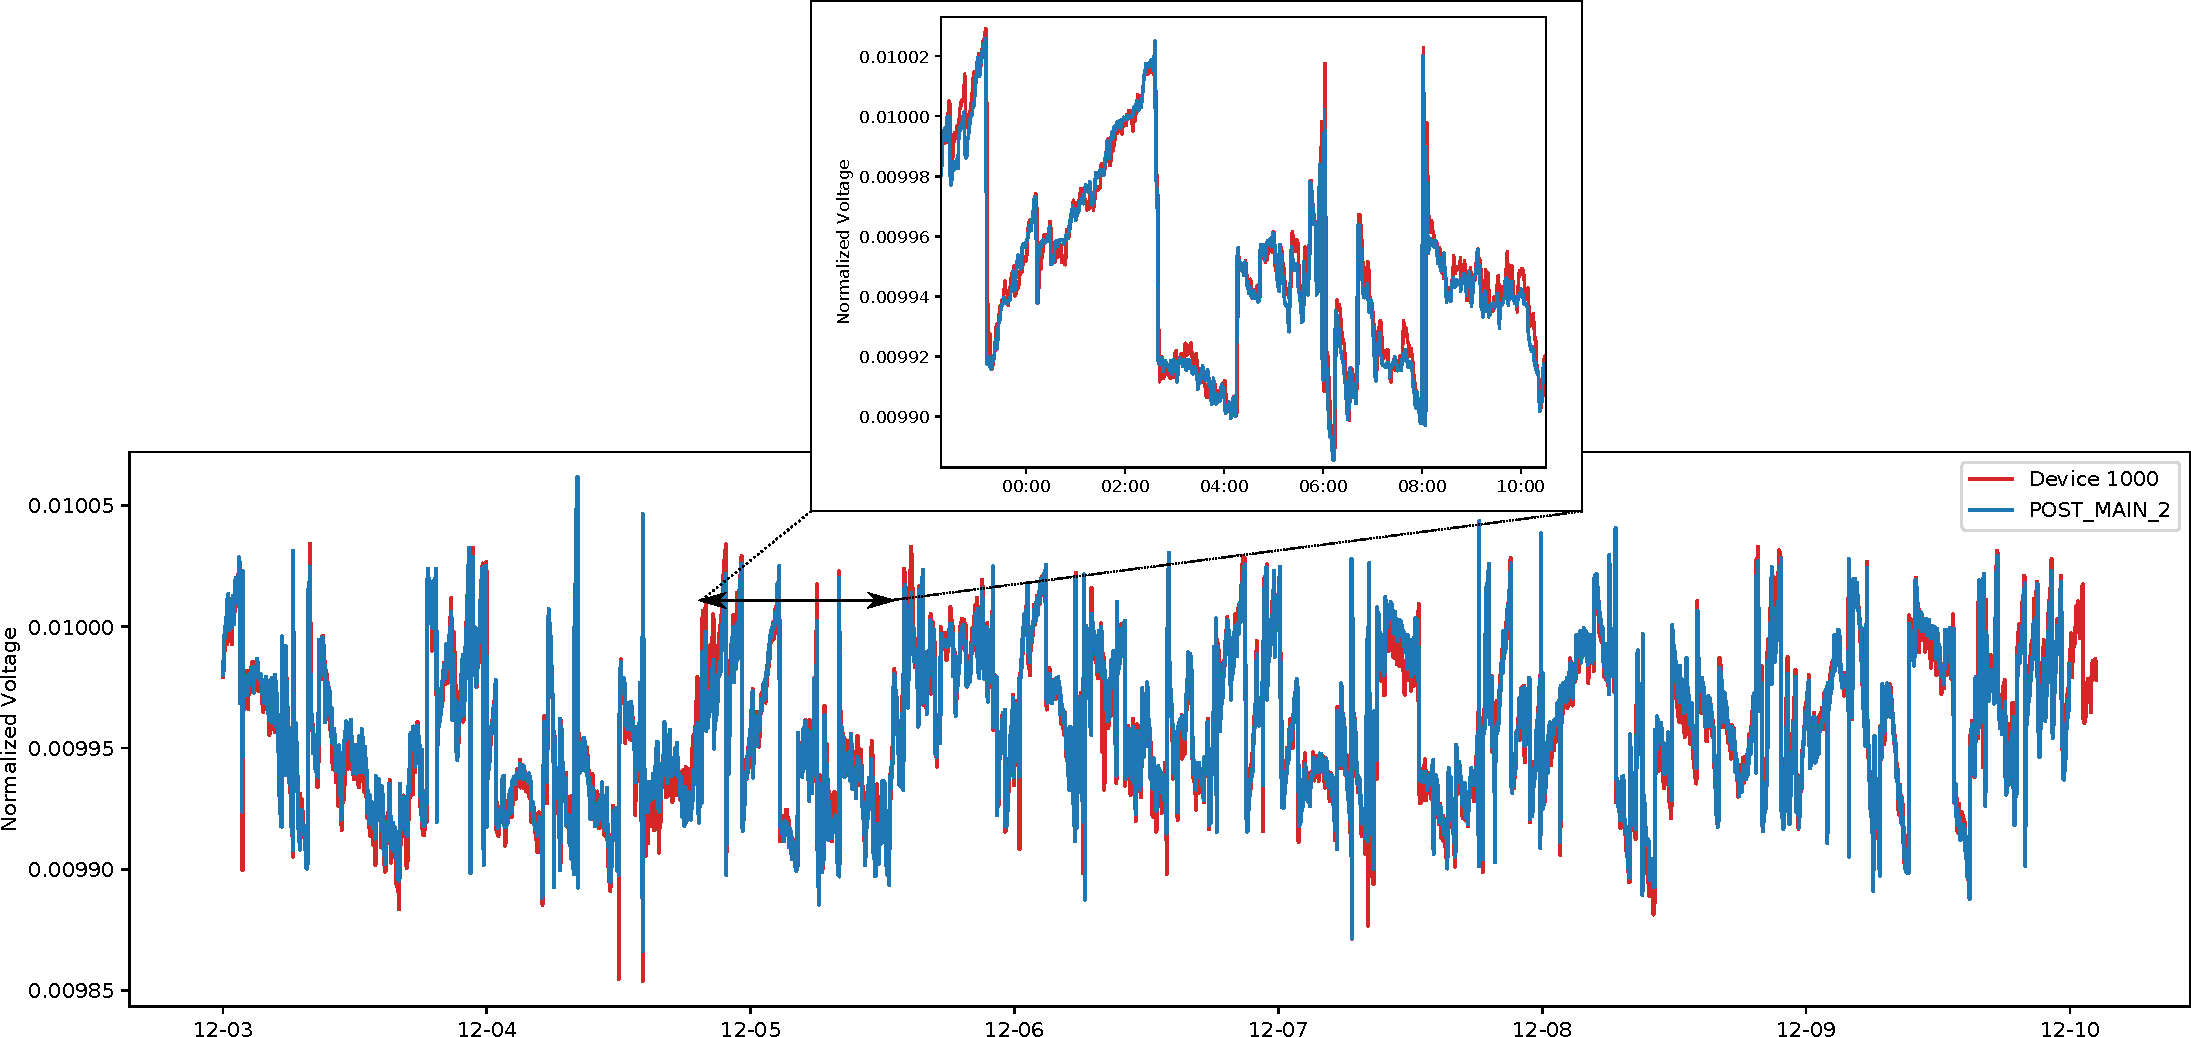
\includegraphics[width=1\linewidth]{img/napali_eval/gt/gt_rms.pdf}
    \caption{RMS metric for the POST\_MAIN\_2 utility meter and OPQ Box 1000.}
    \label{expdes:fig:postmain2:rms}
\end{figure}

It should be noted that the $V_{rms}$ for POST\_MAIN\_2 shown in Figure \ref{expdes:fig:postmain2:rms} is not the raw waveform acquired from the meter.
The raw data consists of the inter-phase across between each leg of the 3 phase system.
Typically, in order to step down a 3 phase 480V system into a 120V single phase a star or a delta transformer is employed.
The voltage generated from this transform configuration is a quadrature combination of the three phases \cite{Horowitz:2015:AE:2960712}, thus the voltage displayed in Figure \ref{expdes:fig:postmain2:rms} was in fact:

\begin{equation}\label{eq:v_rms_3phase_to_signle}
\begin{aligned}
    V_{rms} = \frac{1}{\sqrt{3}C}\sqrt{V_{ab}^2 + V_{bc}^2 +V_{ca}^2}
\end{aligned}
\end{equation}
where the $V_{ab}$, $V_{bc}$ and $V_{ca}$ are the inter-phase voltages reported by the meter, and C is a constant dependent on the transformer configuration and the final step down voltage.
In order to make the differences stand out across the two scales Figure \ref{expdes:fig:postmain2:rms} was generated with both data sets normalized.
A typical step down turn ratio of 480V to 120V is naturally 4:1, which matches quite well with the measured step down factor extracted from the OPQ data and result of Equation \ref{eq:v_rms_3phase_to_signle} of 3.9985:1.

Just as with Frequency and THD metrics we compared the difference between the between the reported voltage by the two devices.
Equation \ref{eq:v_rms_3phase_to_signle} was used along with the empirically measured $C = 3.9985$ in order to preprocess the POST\_MAIN\_2 dataset.
The resulting histogram is shown in Figure \ref{expdes:fig:postmain2:rms_diff}

\begin{figure}[ht!]
    \centering
    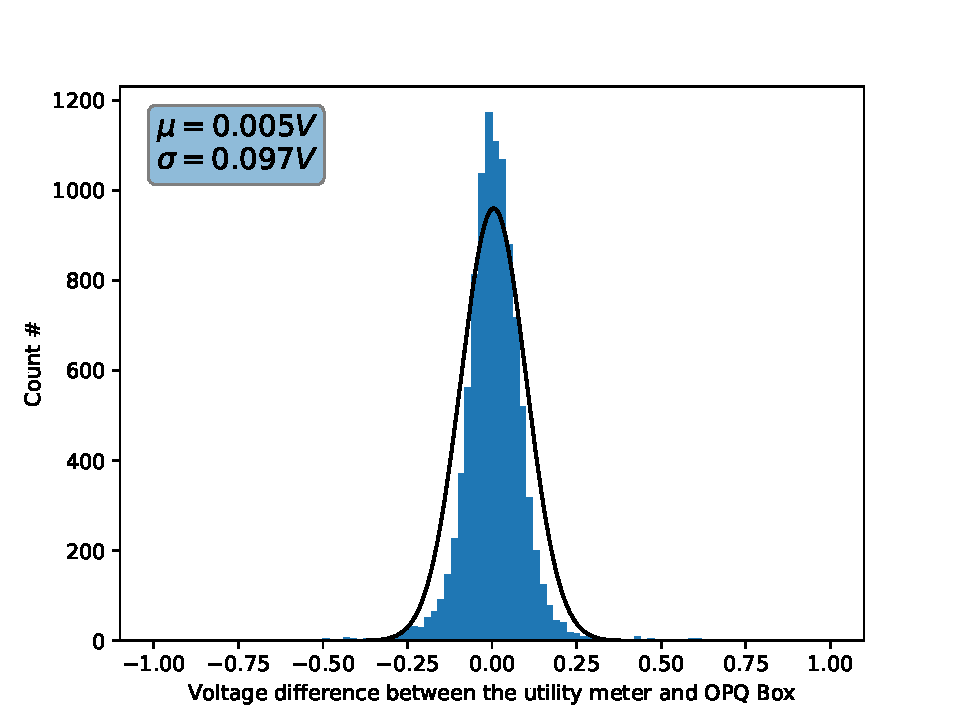
\includegraphics[width=0.7\linewidth]{img/napali_eval/gt/gt_rms_diff.pdf}
    \caption{Difference in the $V_{rms}$ metric between POST\_MAIN\_2 utility meter and OPQ Box 1000.}
    \label{expdes:fig:postmain2:rms_diff}
\end{figure}

There were a few outliers, resulting in a poor fit.
These outliers were likely due to the timing misalignment in the device data.
While overall timing agrees quite well, the meters report their metric at one minute averages, similar to the OPQ Box.
However, when the minute begins and ends is quite arbitrary for the OPQ Box, thus resulting in some overlap.
Regardless, even with the timing discrepancy the voltage metrics agree to an excellent degree across both devices with a $\sigma=0.1V$.
With the event threshold of $\pm5V$ this level of agreement was found to be acceptable.

\paragraph{Overall metric comparison:}
Metrics between the utility meter and the OPQ device were found to correlate to a great degree of accuracy.
Frequency measurements in particular was well formed, with a well characterized gaussian with minimal offset and a $\sigma =8mHz$.
Total harmonic distortion tracked very well across the devices, with the difference $\sigma < 0.04\%$ in all cases.
However, additional offset was regularly introduced by some form of harmonic filtering equipment.
$V_{rms}$ voltage agreement across the two devices suffered the most as expected.
There is no way to analytically calculate the step down factor between the 480V three phase system and 120V system without taking apart and measuring the power transformer which powers the POST building.
However the empirically measured turn ratio matched closely to the expected value.
Furthermore, two meters were in close agreement at all times with $\sigma =0.1V$ between the two devices.
This discrepancy was expected, since both devices are influenced by a different noise sources, with the POST\_MAIN\_2 meter noise being a superset of that observed by the OPQ Box 1000.
The performance of the metric extraction, compared to the utility meter, was found to be satisfactory across the board, making the OPQ Box well suited for grid edge power quality monitoring.

\subsubsection{Gridwide event extraction from utility meters}
\begin{center}
    \begin{table}[!ht]
        \caption{OPQ Box and utility meter collocation. }
        \label{tbl:expdes:meter_colocation}
        \begin{tabularx}{\textwidth}[t]{sb}
            \textbf{OPQ Box ID} &\textbf{Utility Meter}\\
            \arrayrulecolor{black}\hline
            1000, 1002 & POST\_MAIN\_1 \newline
            POST\_MAIN\_2\\
            \arrayrulecolor{black}\hline
            1001 & HAMILTON\_LIB\_PH\_III\_CH\_1\_MTR \newline
            HAMILTON\_LIB\_PH\_III\_CH\_2\_MTR \newline
            HAMILTON\_LIB\_PH\_III\_CH\_3\_MTR \newline
            HAMILTON\_LIB\_PH\_III\_MAIN\_1\_MTR \newline
            HAMILTON\_LIB\_PH\_III\_MAIN\_2\_MTR \newline
            HAMILTON\_LIB\_PH\_III\_MCC\_AC1\_MTR \newline
            HAMILTON\_LIB\_PH\_III\_MCC\_AC2\_MTR \\
            \arrayrulecolor{black}\hline
            1003 & KELLER\_HALL\_MAIN\_MTR\\
            \arrayrulecolor{black}\hline
            1021 & MARINE\_SCIENCE\_MAIN\_A\_MTR \newline
            MARINE\_SCIENCE\_MAIN\_B\_MTR \newline
            MARINE\_SCIENCE\_MCC\_MTR \\
            \arrayrulecolor{black}\hline
            1022 & AG\_ENGINEERING\_MAIN\_MTR \newline
            AG\_ENGINEERING\_MCC\_MTR \\
            \arrayrulecolor{black}\hline
            1023 & LAW\_LIB\_MAIN\_MTR \\
            \arrayrulecolor{black}\hline
            1025 & KENNEDY\_THEATRE\_MAIN\_MTR \\
        \end{tabularx}
    \end{table}
\end{center}
In addition to POST\_MAIN\_2 several other meters were collocated in the same building as an OPQ Box.
Details of this collocation are shown in Table \ref{tbl:expdes:meter_colocation}.
Data from these utility meters was used as a basis for evaluation of the temporal locality claim of the Napali framework.
Napali temporal locality states that by monitoring the edge nodes of the power grid for temporally related disturbances, the state of the power grid can be determined.
In the next section I show this claim to be true, however, prior to that I demonstrate how gridwide events were extracted from the utility meter records.

As shown in Table \ref{tbl:expdes:meter_colocation} the POST building has two OPQ Devices and two utility meters.
Furthermore, several OPQ devices are located in buildings with more then one meter.
Unfortunately, no detailed building schematics were made available to us, thus it is not clear which meter was a parent node of the OPQ Box in the power grid hierarchy.

\begin{figure}[ht!]
    \centering
    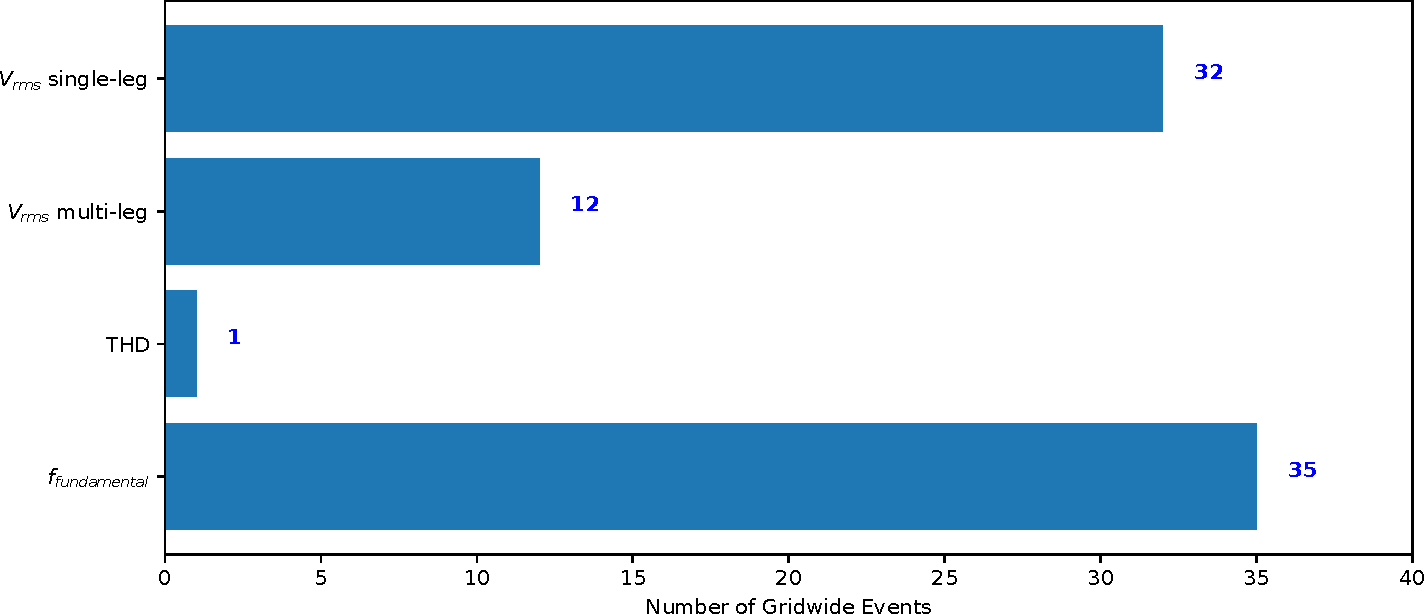
\includegraphics[width=1\linewidth]{img/napali_eval/gt/utility_events_total.pdf}
    \caption{Total number of gridwide and subthreshold events extracted from the utility power meters from November 15th to December 19th.}
    \label{expdes:fig:postmain2:utility_event_total}
\end{figure}

In order to extract anomalies which affected the collocated meters, utility meters from Table \ref{tbl:expdes:meter_colocation} were queried for metrics from November 15th 2019 to December 19th 2019.
These metrics contained minute windowed average, minimum and maximum values for the following power quality measurements:
\begin{enumerate}
    \item $V_{rms}(AB)$, $V_{rms}(BC)$, $V_{rms}(CA)$ : RMS value for the inter-phase voltage.
    \item $f_{fundamental}$ : Fundamental frequency.
    \item $THD$ : Total harmonic distortion.
\end{enumerate}

It is unclear which leg of the three phase system the  $f_{fundamental}$ measurement was performed on.
The THD measurement was likely performed on all three legs and combined together, since it matches closely to the box measurement as shown in Figure \ref{expdes:fig:postmain2:thd} and \ref{expdes:fig:postmain2:thd_diff}.
Finally, in a few meters lacked the $V_{rms}(AB)$, $V_{rms}(BC)$ and $V_{rms}(AB)$ and instead delivered $V_{rms}(AN)$, $V_{rms}(BN)$, $V_{rms}(CN)$ measurements.
These measurements are line-to-neutral instead of line to line.
In these caseses, instead of using equation \ref{eq:v_rms_3phase_to_signle}, Equation \ref{eq:v_rms_3phaseN_to_signle} to calculate observed 120V line voltage. \cite{Horowitz:2015:AE:2960712}

\begin{equation}\label{eq:v_rms_3phaseN_to_signle}
\begin{aligned}
    V_{rms} = \frac{\sqrt{3}}{4}\sqrt{V_{ab}^2 + V_{bc}^2 +V_{ca}^2}
\end{aligned}
\end{equation}

\begin{figure}[ht!]
    \centering
    \begin{subfigure}{.45\textwidth}
        \centering
        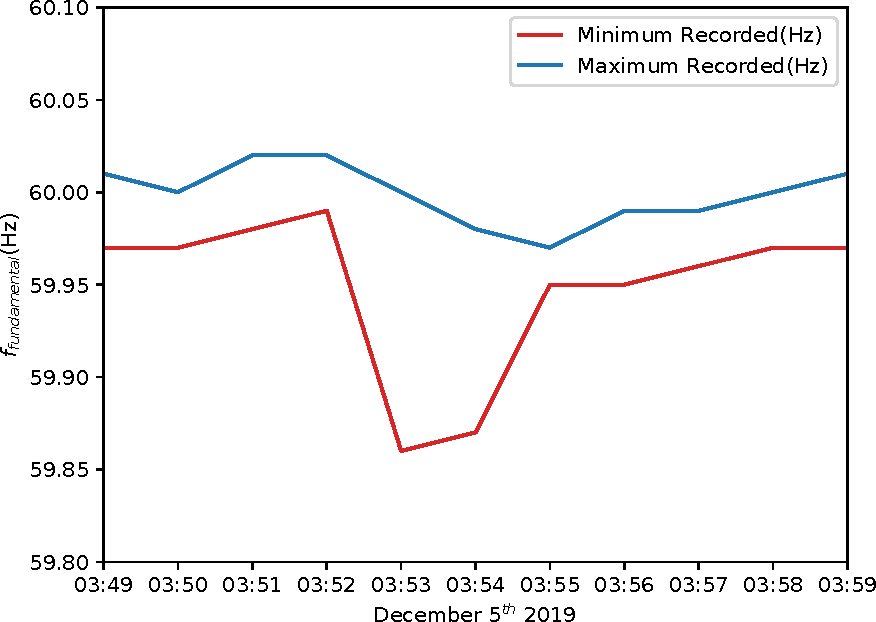
\includegraphics[width=1\linewidth]{img/napali_eval/gt/gt_f_example.pdf}
        \caption{}
        \label{expdes:fig:gt_example:f}
    \end{subfigure}\hspace{5mm}
    \begin{subfigure}{.45\textwidth}
        \centering
        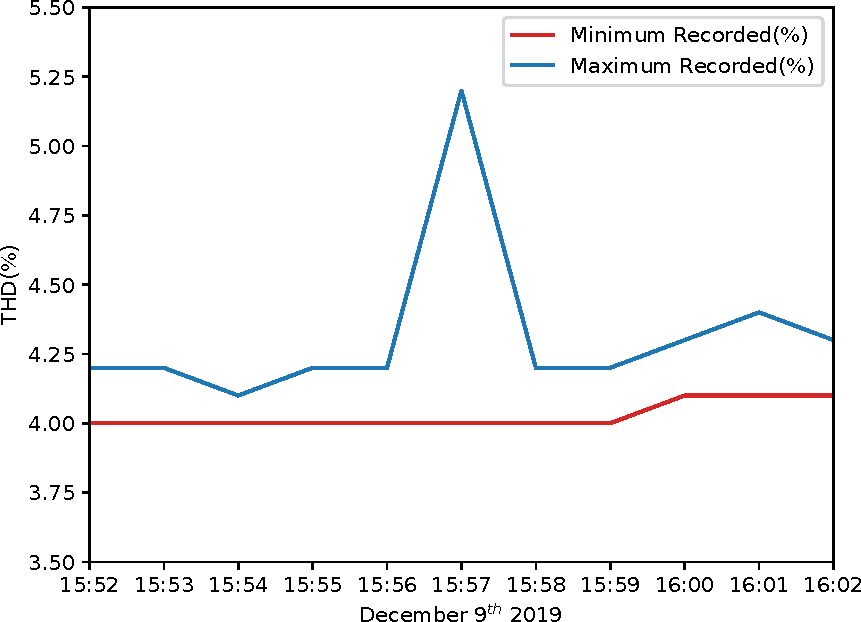
\includegraphics[width=1\linewidth]{img/napali_eval/gt/gt_thd_example.pdf}
        \caption{}
        \label{expdes:fig:gt_example:thd}
    \end{subfigure}
    \begin{subfigure}{.45\textwidth}
        \centering
        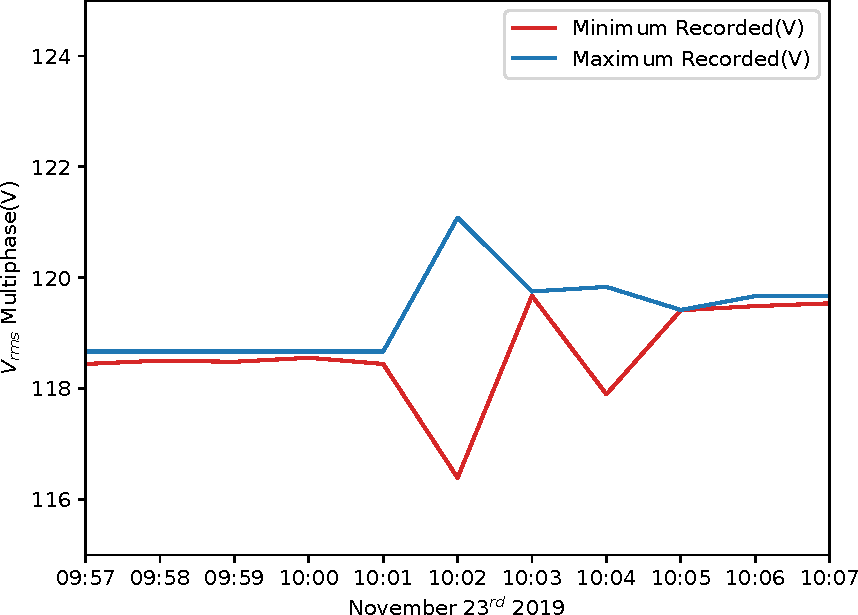
\includegraphics[width=1\linewidth]{img/napali_eval/gt/gt_vpoly_example.pdf}
        \caption{}
        \label{expdes:fig:gt_example:vpoly}
    \end{subfigure}\hspace{5mm}
    \begin{subfigure}{.45\textwidth}
        \centering
        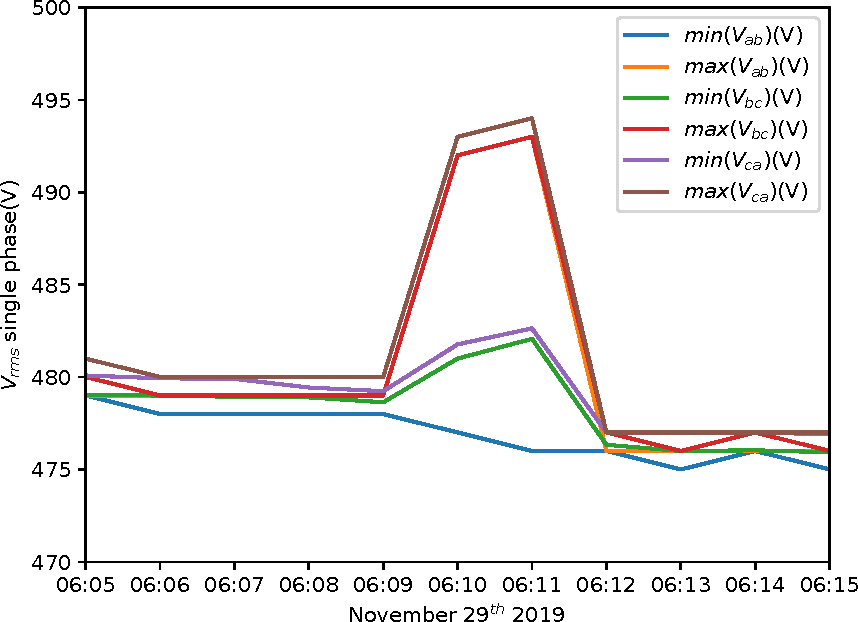
\includegraphics[width=1\linewidth]{img/napali_eval/gt/gt_vsingle_example.pdf}
        \caption{}
        \label{expdes:fig:gt_example:vsingle}
    \end{subfigure}

    \caption{Example of the four types of events extracted from utility meter data.
    a)Fundamental frequency event recorded by POST\_MAIN\_2.
    b) THD event recorded by HAMILTON\_LIB\_PH\_III\_MAIN\_1.
    c) Multiphase $V_{rms}$ event as recorded by HAMILTON\_LIB\_PH\_III\_CH\_2.
    d) Single phase $V_{rms}$ event as recorded by HAMILTON\_LIB\_PH\_III\_CH\_3.}

    \label{expdes:fig:gt_example}
\end{figure}

Extraction for $f_{fundamental}$ and $THD$ metrics were processed in a similar manner to the OPQ Box events.
If the minimum or maximum metric exceeded the threshold defined in Table \ref{tbl:opq:thresholds} were surpassed, the temporal region was marked as anomalous.
If anomalous regions across multiple utility meters were marked, that temporal region was reported as a utility gridwide event.
$V_{rms}$ measurements were processed in a slightly different manner.
First, the $V_{rms}$ value as observed by the OPQ devices was calculated from both minimum and maximum of the utility metrics using Equation \ref{eq:v_rms_3phaseN_to_signle} or \ref{eq:v_rms_3phase_to_signle}.
These values were then treated in the same manner as $f_{fundamental}$ and $THD$.
Next the individual phases $V_{rms}(AB)$, $V_{rms}(BC)$, $V_{rms}(CA)$ or $V_{rms}(AN)$, $V_{rms}(BN)$, $V_{rms}(CN)$ were thresholded using the same $8\frac{1}{3}\%$ threshold used for the OPQ devices.
If more then one utility meter observed a single phase sag or swell it was marked as a utility gridwide event.

Total number of events of each type extracted from the utility meters is shown in Figure \ref{expdes:fig:postmain2:utility_event_total}.
Examples of recorded gridwide events as observed by various meters is shown in Figure \ref{expdes:fig:gt_example}.

\subsubsection{Evaluation of detection capabilities for the Napali framework}

With the gridwide events extracted from the utility meters in the previous section, a detailed evaluation of Napali detection capabilities was carried out.
Events timestamps which corresponded to the utility meter grid wide events were queried against OPQ event database and analyzed.
Primarily, if an event was located it was reanalyzed to validate that the metric which triggered the utility meter was the same as the one which triggered the OPQ system.

\paragraph{Frequency Gridwide Events:} Out of 35 gridwide frequency events 34 were detected by Napali.
As expected, since frequency is quite consistent across the entire power grid, all OPQ devices triggered on the 34 recorded events.
The missed frequency event occurred on November 25th at 7:08:00 AM which corresponds to a complete 3 minute power outage as shown in Figure \ref{expdes:fig:gt_outage}.
Unfortunately, by the time the OPQ devices finished their initialization procedure, the grid conditions have returned to normal.
It should be noted that the outage was recorded and reported by the OPQ system.

\begin{figure}[ht!]
    \centering
    \begin{subfigure}{.45\textwidth}
        \centering
        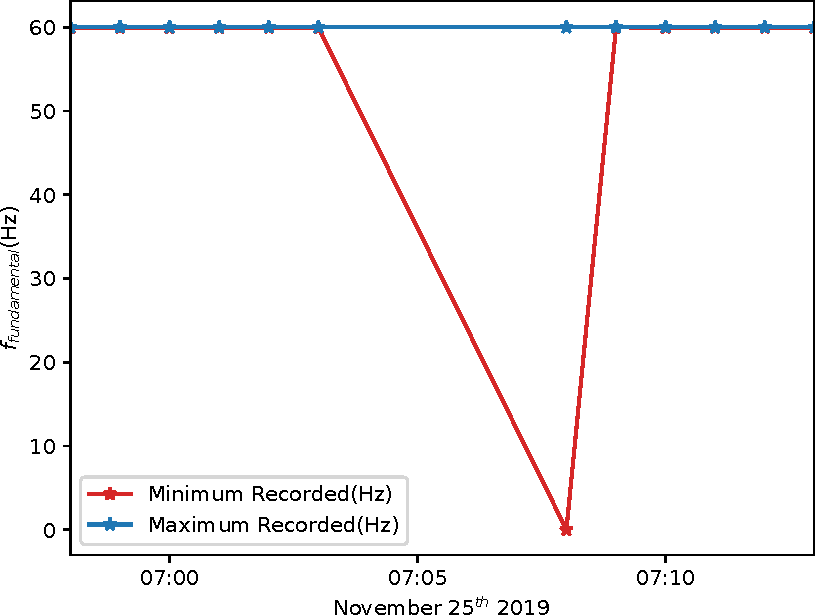
\includegraphics[width=1\linewidth]{img/napali_eval/gt/outage_f.pdf}
        \caption{}
        \label{expdes:fig:gt_outage:f}
    \end{subfigure}\hspace{5mm}
    \begin{subfigure}{.45\textwidth}
        \centering
        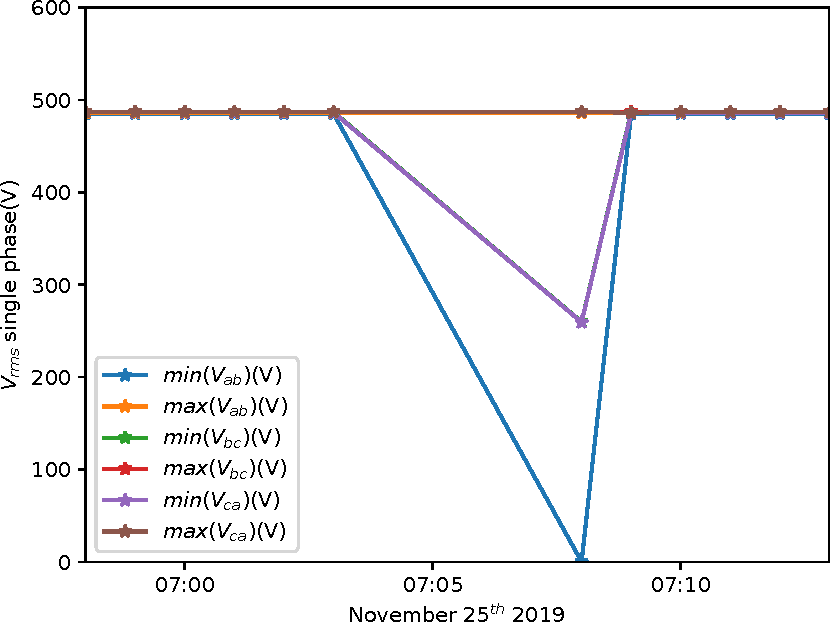
\includegraphics[width=1\linewidth]{img/napali_eval/gt/outage_v.pdf}
        \caption{}
        \label{expdes:fig:gt_outage:v}
    \end{subfigure}

    \caption{November 25th outage as observed by the utility meter POST\_MAIN\_2.
    a) Observed frequency.
    b)Observed voltage.}

    \label{expdes:fig:gt_outage}
\end{figure}

\paragraph{THD gridwide event:} A single THD event extracted from the utility meters was recorded and by the OPQ system with every device sending raw waveforms for the event.

\paragraph{$V_{rms}$ multiphase:} Out of 12 gridwide utility events only 7 were detected by the OPQ system.
However, a closer examination of missed events revealed a pattern.
The table of the missed events and their triggered meters is shown in Table \ref{tbl:expdes:v_rms:missed_events}

\begin{center}
    \begin{table}[!ht]
        \caption{Missed $V_{rms}$ multiphase utility events. }
        \label{tbl:expdes:v_rms:missed_events}
        \begin{tabularx}{\textwidth}[t]{sb}
            \textbf{Event Timestamp} &\textbf{Triggered utility meter}\\
            \arrayrulecolor{black}\hline
            November 26 14:53 & HAMILTON\_LIB\_PH\_III\_CH\_1\_MTR \newline
            HAMILTON\_LIB\_PH\_III\_CH\_3\_MTR \newline
            HAMILTON\_LIB\_PH\_III\_MCC\_AC1\_MTR  \newline
            HAMILTON\_LIB\_PH\_III\_MCC\_AC2\_MTR \\
            \arrayrulecolor{black}\hline
            November 27 11:15 & 	HAMILTON\_LIB\_PH\_III\_CH\_1\_MTR \newline
            HAMILTON\_LIB\_PH\_III\_MAIN\_1\_MTR \newline
            HAMILTON\_LIB\_PH\_III\_CH\_3\_MTR \newline
            HAMILTON\_LIB\_PH\_III\_MCC\_AC1\_MTR \newline
            HAMILTON\_LIB\_PH\_III\_MCC\_AC2\_MTR \\
            \arrayrulecolor{black}\hline
            November 27 11:21 & 	HAMILTON\_LIB\_PH\_III\_CH\_1\_MTR \newline
            HAMILTON\_LIB\_PH\_III\_MAIN\_1\_MTR \newline
            HAMILTON\_LIB\_PH\_III\_CH\_3\_MTR \newline
            HAMILTON\_LIB\_PH\_III\_MCC\_AC1\_MTR \newline
            HAMILTON\_LIB\_PH\_III\_MCC\_AC2\_MTR \\
            \arrayrulecolor{black}\hline
            November 27 15:18 & 	HAMILTON\_LIB\_PH\_III\_CH\_1\_MTR \newline
            HAMILTON\_LIB\_PH\_III\_MAIN\_1\_MTR \newline
            HAMILTON\_LIB\_PH\_III\_CH\_3\_MTR \newline
            HAMILTON\_LIB\_PH\_III\_MCC\_AC1\_MTR \newline
            HAMILTON\_LIB\_PH\_III\_MCC\_AC2\_MTR \\
            \arrayrulecolor{black}\hline
            November 25, 7:08 & All utility meters. \\
        \end{tabularx}
    \end{table}
\end{center}
It seems that between 2pm November $26^{th}$ and 3:30pm November $27^{th}$ electrical equipment in Hamilton library was experiencing power quality issues, while the rest of the University power grid exhibited nominal behaviour.
Since only a single OPQ Device is located in the Hamilton library, Napali rightfully rejected any power quality metrics observed there as local disturbances.
Finally, November 25, 7:08 signifies the power interruption as discussed previously.
As such the true utility gridwide event number is 8 with 7 detected using the Napali framework.

\paragraph{$V_{rms}$ single phase:}
Out of 32 single phase gridwide events, 23 were detected by the Napali framework.
Similarly to the $V_{rms}$ multiphase events:
\begin{itemize}
    \item 1 event was due to the Nov 25 outage.
    \item 6 events were incorrectly classified as gridwide, since they originated from the same building.
\end{itemize}
Two events occurring on November $26^{th}$ 14:53 and November $27^{th}$ 11:15  were missed by the OPQ system.
These events triggered on all of the Hamilton library meters and the KELLER\_HALL\_MAIN\_MTR located in Keller hall.
While one of the phases did go bellow the $\approx 8\%$ threshold, it did not cause a large enough disturbance to appear as an anomaly to the keller hall device.
Furthermore, while these events impacted multiple meters, they during the anomalous period experienced by the Hamilton library subgrid.
It is unlikely that these events were true gridwide events, but instead the bleed over from the Hamilton library.

\subsubsection{Detection capabilities for the Napali framework}
\begin{figure}[!ht]
    \centering
    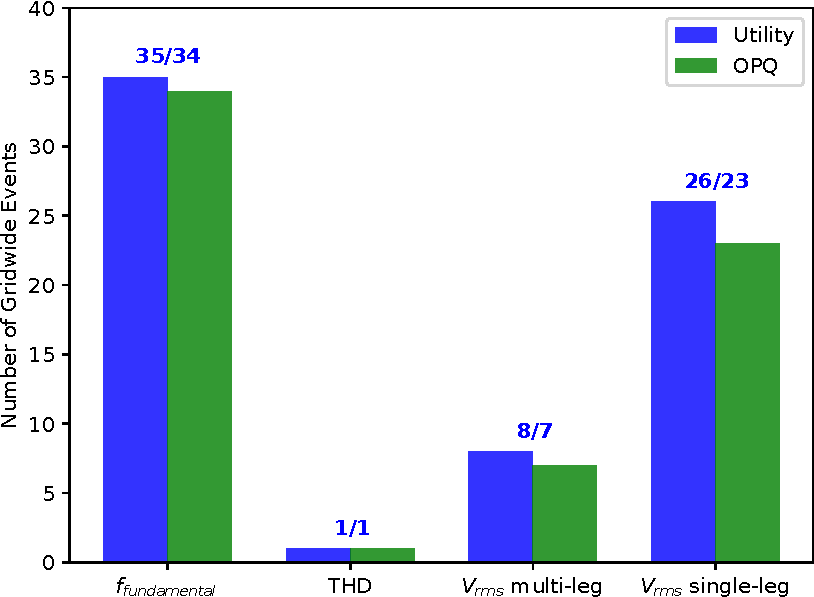
\includegraphics[width=0.9\linewidth]{img/napali_eval/gt/money_plot1.pdf}
    \caption{Comparison of the gridwide events detected by napali and the utility meters.}
    \label{expdes:fig:gt_money}
\end{figure}

The events missed due to the power outage could have been remedied by inclusion of a battery in the OPQ Box.
However, even without the battery, OPQ system was able to correctly identify the power outage.
Disregarding the multi-utility meter events which originated from the same building, detection performance of the Napali framework is outlined in Figure \ref{expdes:fig:gt_money}.
This result validates the temporal locality hypothesis.
Disregarding the event caused by the power outage, Napali showed an over 97\% detection rate for grid wide events.
The two events that were missed by the Napali framework, only affected a single phase of a neighbouring building, and did not cause significant drop in the observed line voltage.

\subsection{Sub-threshold Data Acquisition}\label{subsec:sub-threshold-data-acquisition}

While the Naive method compares favorably to Napali when it comes to resource consumption as outlined in Section \ref{subsec:summary-of-computational-and-network-recource-utilisaztion}, it lacks the ability to detect portions of gridwide events which are below the device detection threshold.
Unlike the Naive method, Napli cooperative edge centric event detection attempts to capture both over-threshold and sub-threshold data as described in Section \ref{subsec:napali-trigger}.
Section \ref{subsec:temporal-locality-triggering-of-the-napali-framework} described the detection capabilities of the OPQ Network and Napali, when detecting partial gridwide events with consensus of 2 or more utility meters.
These are the types of events that the Naive and Napali are equally capable of detecting.
Indeed, the Naive plugin in Makai received data from devices which were collocated with utility meters which observed the disturbance.
In contrast Napali  captured additional waveforms which corresponded to the sub-threshold portions of each event.
More interesting however, were the gridwide events which were extracted from all of the utility meters, not just the ones collocated with an OPQ box.
Particularly, gridwide events which corresponded to an over-threshold anomaly observed by a collocated utility meter as well as one or more of the non-collocated meters were of particular interest.
These events are invariably gridwide, since more then one UH Utility meter was affected, however only a subset of OPQ devices would experience the disturbance with an over-threshold severity.
This is a subtle difference from events used in the previous section.
In order to perform this evaluation a dataset of ground thruth validated partial gridwide events was required, and the only way to obtain it was by filtering Utility meter data to temporal windows consisting of:
\begin{itemize}
    \item \textbf{One over-threshold collocated utility meter:} This made sure that one of the metrics from a collocate OPQBox passed a threshold.
    \item \textbf{One or more over-threshold non-collocated utility meters:} This allowed us to conclude that the event was partial gridwide event.
\end{itemize}
These events create a basis for sub-threshold data acquisition false negative analysis.
After all, it is clearly established that these events are gridwide, and affect only a portion of the UH power delivery infrastructure.
If Napali is capable of locating and acquiring subthreshold portions of these events, it would prove the claim that the subthreshold event acquisition is both a possible and useful tool for power quality analysis.

\begin{center}
    \begin{table}[!ht]
        \caption{Gridwide events with collocated and non-collocated meters which impacted only a portion of the power grid}
        \label{tbl:expdes:sub:colononcolo}
        \begin{tabularx}{\textwidth}[t]{p{2.5cm}|p{2.8cm}|p{7.2cm}|b}
            \textbf{Time} &\textbf{Collocated } & \textbf{Non-collocated} & \textbf{OPQBox}\\
            \arrayrulecolor{black}\hline
            Nov 24 7:57 & POST\_MAIN\_2 & BUS\_AD\_SHIDLER\_MAIN\_MTR \newline
            ST\_JOHN\_PLANT\_SCIENCE\_MAIN\_MTR \newline
            MOORE\_HALL\_MAIN\_MTR \newline
            HPER\_KLUM\_GYM\_MTR \newline
            MULTIPURPOSE\_BLDG\_MAIN\_MTR \newline &
            All\\
            \arrayrulecolor{black}\hline

            Nov 29 6:10 & POST\_MAIN\_2 & MULTIPURPOSE\_BLDG\_MAIN\_MTR &
            1000 \newline
            1002 \newline
            1005 \newline
            1006 \newline
            1007 \newline
            1010 \newline
            1021 \newline
            1022 \newline
            1023 \newline
            1024 \\
            \arrayrulecolor{black}\hline
            Dec 14 13:14 & POST\_MAIN\_2 & BUS\_AD\_SHIDLER\_MAIN\_MTR \newline
            ST\_JOHN\_PLANT\_SCIENCE\_MAIN\_MTR \newline
            MOORE\_HALL\_MAIN\_MTR \newline &
            1000 \newline
            1005 \newline
            1006 \newline
            1007 \newline
            1010 \newline
            1021 \newline
            1022 \newline
            1023 \newline
            1024\\
            \arrayrulecolor{black}\hline
        \end{tabularx}
    \end{table}
\end{center}

Unfortunately, events which impact only a part of the UH power grid with the affected area limited to a region with both collocated and non-collocated meters are quite rare.
From the data made available to us from the UH Smart meters only 3 such events were identified.
These events are shown in Table \ref{tbl:expdes:sub:colononcolo}.

It is unclear why these events all seem to have similar parent Utility meters.
Nonetheless, two of the events have data from every device on the OPQ network.
The other two events only impacted 9 and 10 out of 15 deployed devices respectively.
Another peculiarity is that POST\_MAIN\_2 and POST\_MAIN\_1 utility meters service the same building, however, POST\_MAIN\_1 was not affected enough to qualify for these events.
In the next sections these events are examined in more detail.
\subsubsection{Event 1(Nov 24 7:57 ):}
\begin{figure}[!ht]
    \centering
    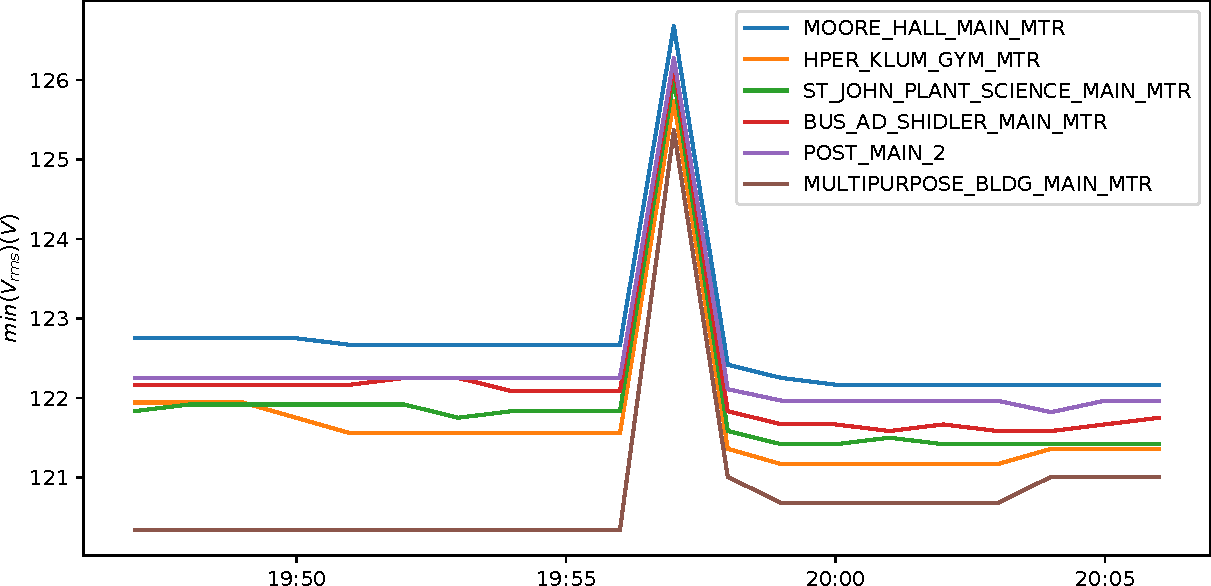
\includegraphics[width=0.7\linewidth]{img/napali_eval/subthreshold/ev1/ev1_gt.pdf}
    \caption{Utility meter data for Event 1}
    \label{expdes:fig:sub:ev1:gt}
\end{figure}
\begin{figure}[!ht]
    \centering
    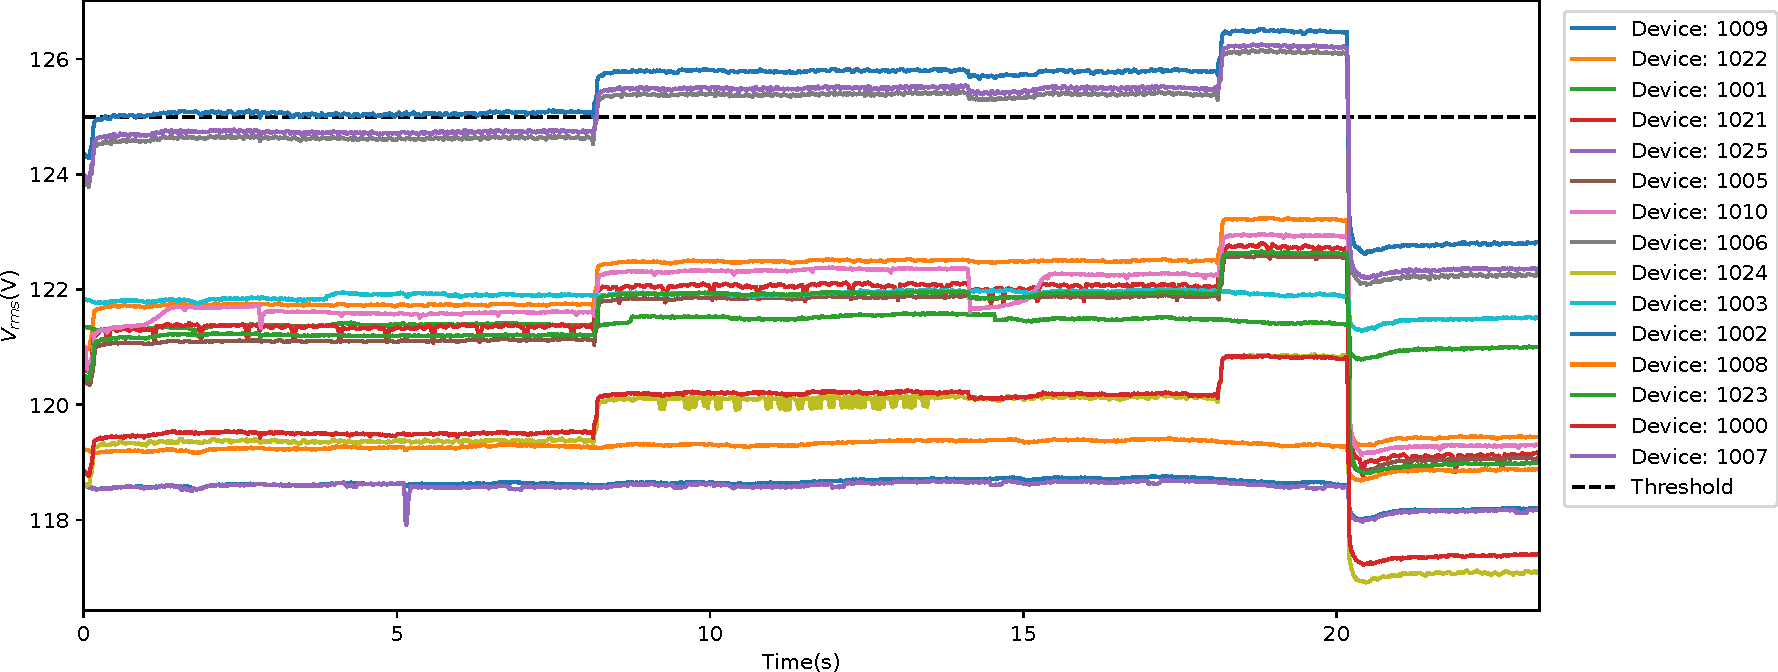
\includegraphics[width=1\linewidth]{img/napali_eval/subthreshold/ev1/boxes_combined.pdf}
    \caption{Napali Event Data for event 1.}
    \label{expdes:fig:sub:ev1:boxes}
\end{figure}
\begin{figure}[!ht]
    \centering
    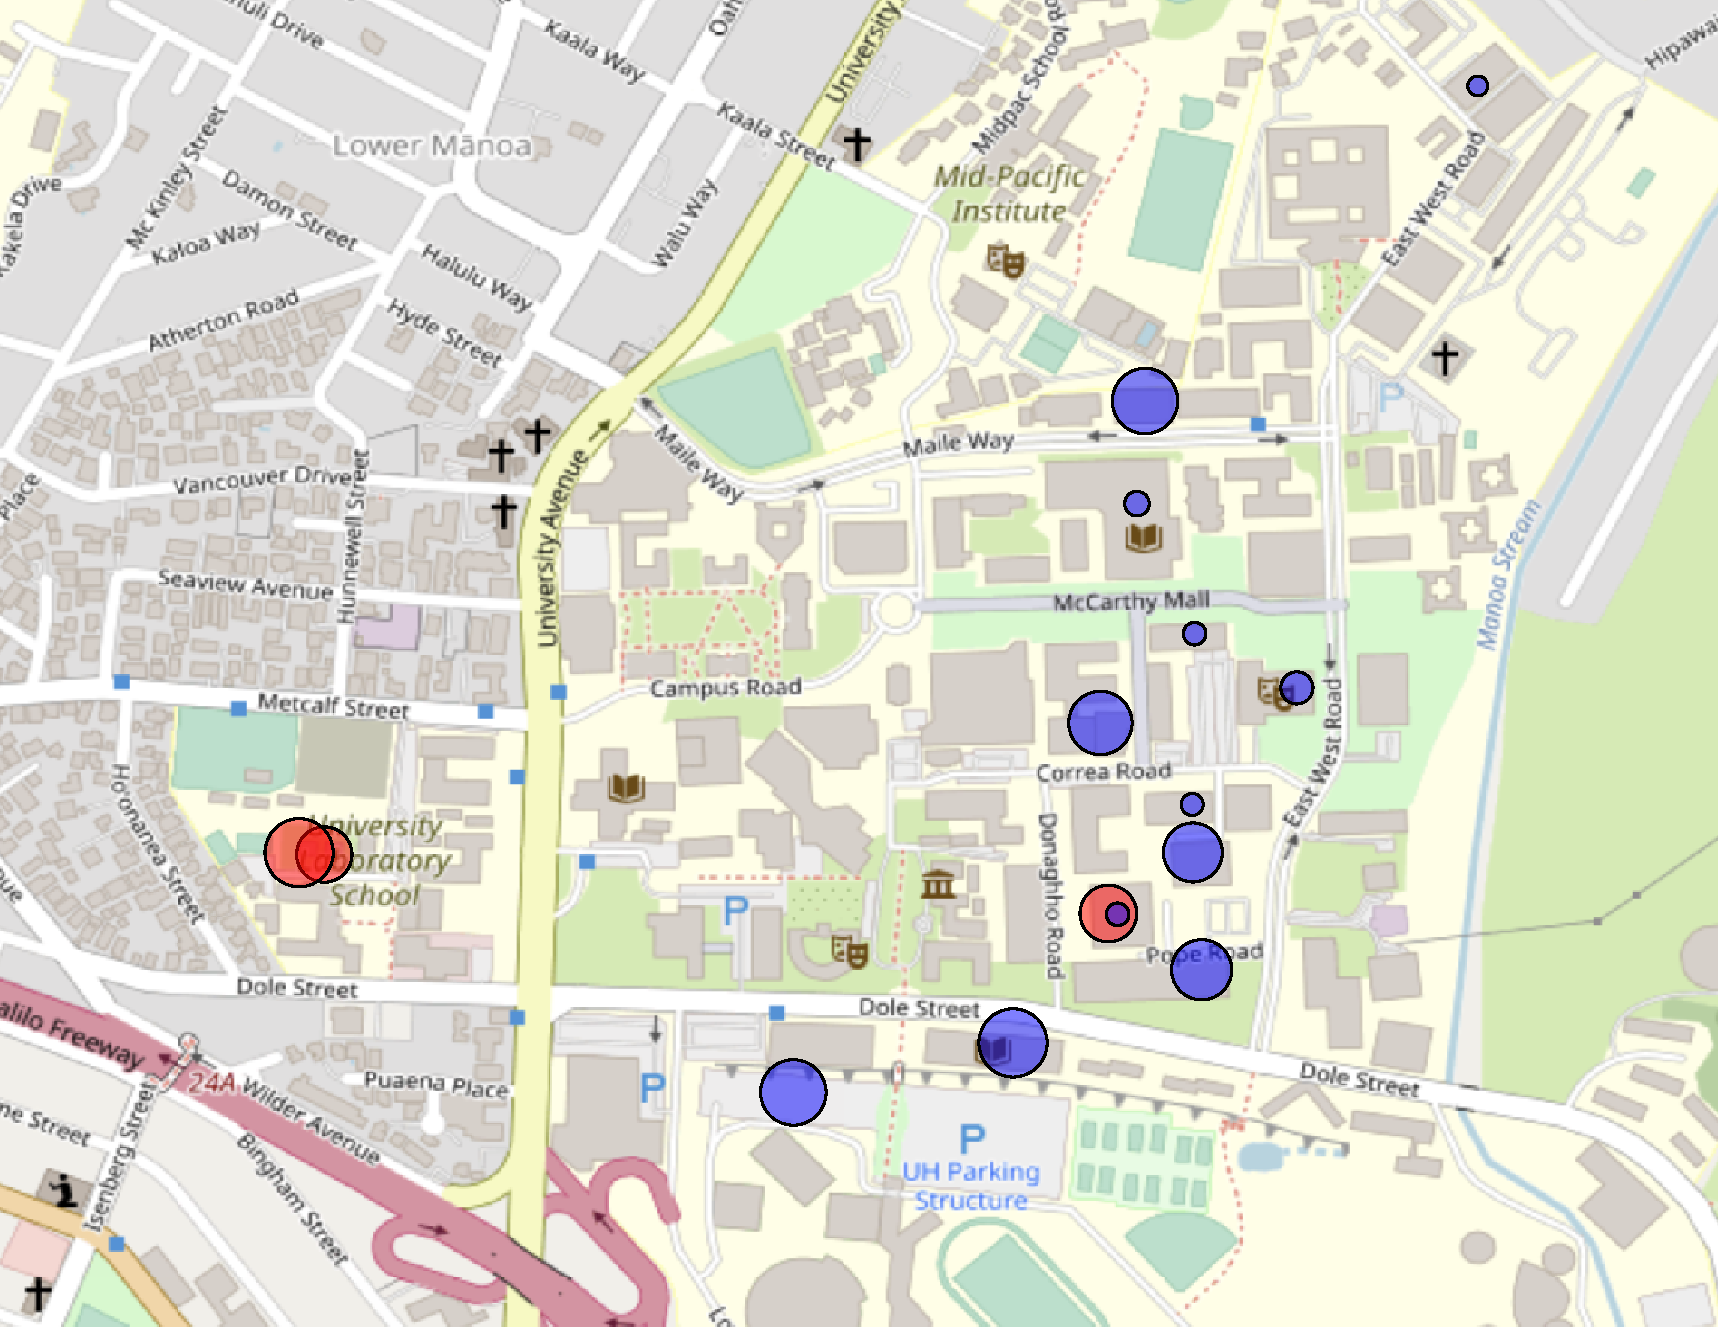
\includegraphics[width=0.7\linewidth]{img/napali_eval/subthreshold/ev1/map.pdf}
    \caption{Geospatial representation of event 1.
    Self-Triggered detected events are shown in red.}
    \label{expdes:fig:sub:ev1:map}
\end{figure}

The $V_{rms}$ for Utility meters registering this event is shown in Figure \ref{expdes:fig:sub:ev1:gt}.
This event was characterized as a large voltage swell, affecting a large portion of the campus.
The voltage anomaly was significant enough to trigger OPQ Box devices 1006, 1007 and 1002 using the Self-Triggering method making it a partial gridwide event.
In contrast the Napali acquired data from  all of the UH devices.
Figure \ref{expdes:fig:sub:ev1:boxes} is a 1 cycle $V_{rms}$ calculated from the raw data acquired from the OPQ Devices by Napali.
The threshold displayed as a dashed line clearly outlines the 3 anomalous devices using the Self-Triggered method, however a similar trend is observed in all other devices.

Another representation of Event 1 is shown in Figure \ref{expdes:fig:sub:ev1:map}.
Here the severity of the event is categorized not by the value over threshold, but instead by the swing between the maximum and minimum of the $V_{rms}$ waveform.
Larger changes in the $V_{rms}$ magnitude are used as a metric of the severity of the event at a particular location.
The size of the circle  in Figure \ref{expdes:fig:sub:ev1:map} represents a larger impact.
Whether the device passed the trigger threshold or not is represented in the color of the circle.
Devices which were triggered via the Self-Triggered method in addition to Napali are shown in red.
Clearly this event looks quite different when acquired via the two methodologies.
From the point of view of the Self-Triggered method, the event only had a limited impact on the power grid with only a small portion of campus affected.
On the other hand, Napali provides a much clearer picture of the event propagation and impact.
In fact the magnitude of the disturbance is just as large in some of the over-threshold and sub-threshold waveforms.
\subsubsection{Event 2(Nov 29 6:10):}
\begin{figure}[!ht]
    \centering
    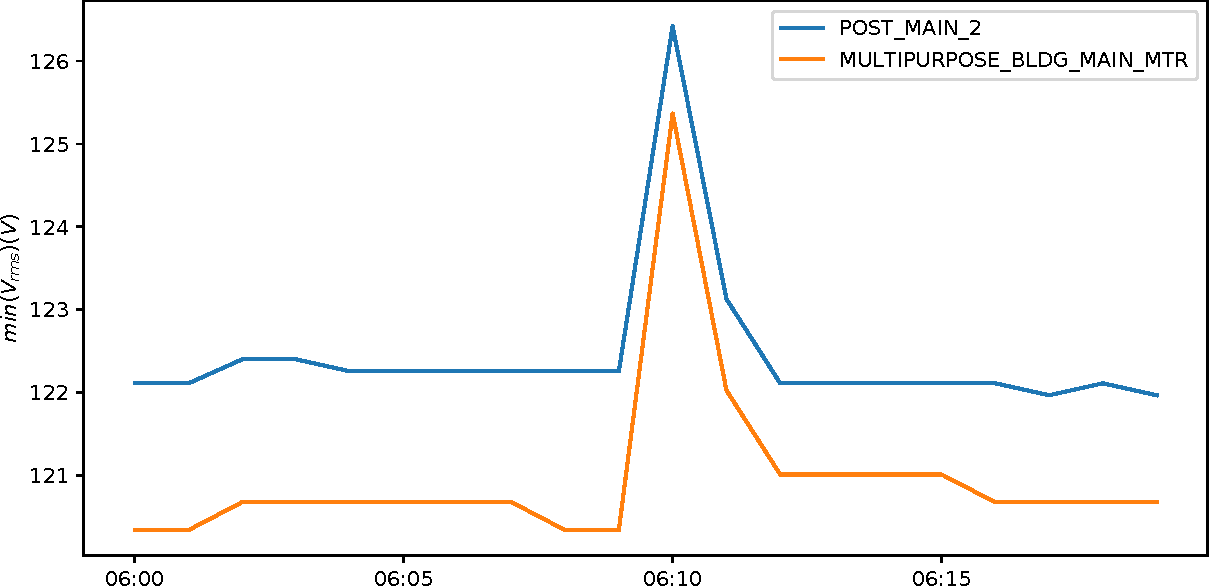
\includegraphics[width=0.7\linewidth]{img/napali_eval/subthreshold/ev2/ev2_gt.pdf}
    \caption{Utility meter data for Event 2.}
    \label{expdes:fig:sub:ev2:gt}
\end{figure}
\begin{figure}[!ht]
    \centering
    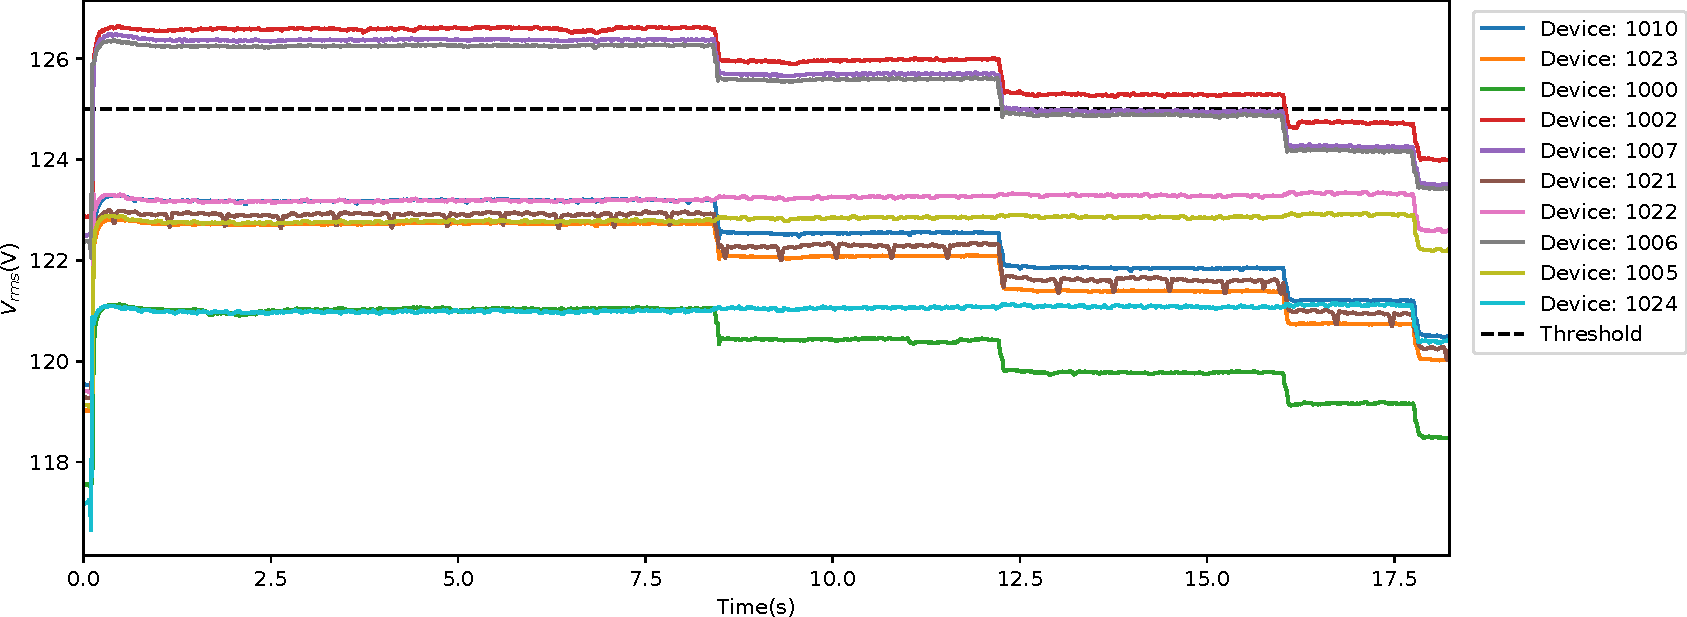
\includegraphics[width=1\linewidth]{img/napali_eval/subthreshold/ev2/boxes_combined.pdf}
    \caption{Napali Event Data for event 2.}
    \label{expdes:fig:sub:ev2:boxes}
\end{figure}
\begin{figure}[!ht]
    \centering
    \begin{subfigure}{.45\textwidth}
        \centering
        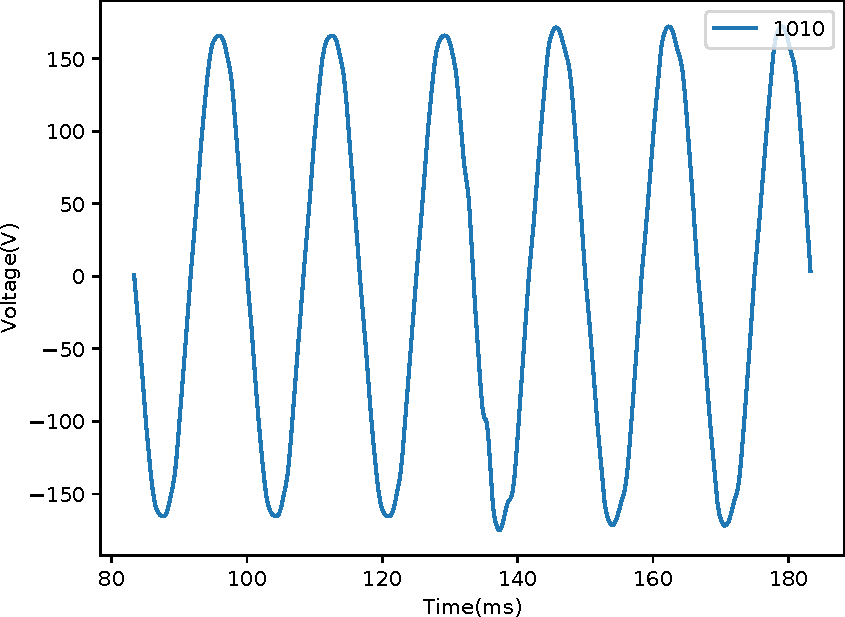
\includegraphics[width=1\linewidth]{img/napali_eval/subthreshold/ev2/trans_1010.pdf}
    \end{subfigure}\hspace{5mm}
    \begin{subfigure}{.45\textwidth}
        \centering
        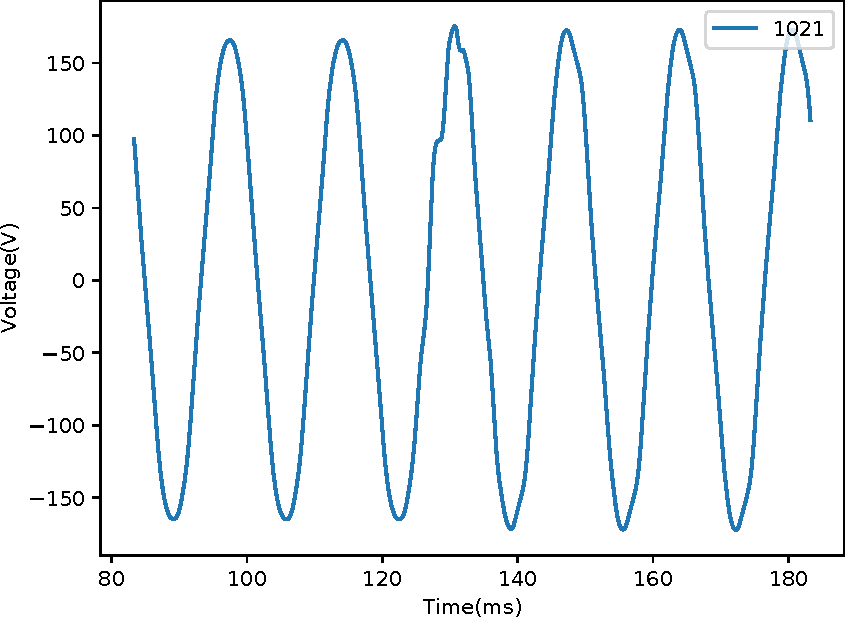
\includegraphics[width=1\linewidth]{img/napali_eval/subthreshold/ev2/trans_1021.pdf}
    \end{subfigure}
    \begin{subfigure}{.45\textwidth}
        \centering
        \includegraphics[width=1\linewidth]{img/napali_eval/subthreshold/ev2/trans_1022.pdf}
    \end{subfigure}\hspace{5mm}
    \begin{subfigure}{.45\textwidth}
        \centering
        \includegraphics[width=1\linewidth]{img/napali_eval/subthreshold/ev2/trans_1024.pdf}
    \end{subfigure}
    \caption{Transients recorded as part of event 2.}
    \label{expdes:fig:sub:ev2:trans}
\end{figure}
\begin{figure}[!ht]
    \centering
    \includegraphics[width=0.7\linewidth]{img/napali_eval/subthreshold/ev2/map.pdf}
    \caption{Geospatial representation of event 2.
    Self-Triggered detected events are shown in red.
    Waveforms containing transients are shown in green.}
    \label{expdes:fig:sub:ev2:map}
\end{figure}

This event was observed by only two Utility Smart meters.
The $V_{rms}$ for Utility meters is shown in Figure \ref{expdes:fig:sub:ev2:gt}.
Similarly to event 1, event 2 was categorized by the Utility meters as a voltage swell.
In continued similarity, same devices: 1006, 1007 and 1002 passed the $V_{rms}$ threshold, and thus were triggered by the Self-Triggering event detection method.
Napali however, triggered 7 additional devices.
The cycle level $V_{rms}$ for the devices detected by Napali is shown in Figure \ref{expdes:fig:sub:ev2:boxes}
While the utility meter data makes Event 1 and Event 2 look quite similar, OPQ data shows them to have an opposing chronological order.
Instead of a slow $V_{rms}$ rise and a fast return to nominal as observed in event 1, event 2 is characterized by a fast $V_{rms}$ rise and a slow decay.

Further analysis indicates that the fast $V_{rms}$ rise at $t=130ms$ is further characterised by a transient observed by 4 OPQ Box devices.
These transients are shown in Figure \ref{expdes:fig:sub:ev2:map}
The transients were small enough to be missed by the Self-Triggered event detection method, yet were captured by Napali.
The geospatial representation of event 2 is shown in Figure \ref{expdes:fig:sub:ev2:map}.
As with event 1, the magnitude of the event is taken as the swing between the minimum and maximum of the $V_{rms}$ waveform.
Event magnitude is represented as the size of the symbol on Figure \ref{expdes:fig:sub:ev2:map}.
Red represents devices triggered by both Napali and the Self-Triggered method.
Blue are events which were triggered only by Napali.
Finally, green color symbols represent events which were triggered by Napali with contained transients.

Event 2 as observed by the Self-Triggered method contains only a small portion of the event.
Waveforms from the same buildings as those affected by event 1 are captured, with no information available regarding the rest of the grid.
The transients are completely missed, and so is the rest of the impacted
locations.

This event looks significantly different when observed via Napali.
The University power gid is divided into three distinct portions.
West portion of campus experienced a $V_{rms}$ swell which surpassed the OPQ imposed threshold.
South portion experienced a $V_{rms}$ swell of a similar magnitude, without passing the threshold.
Finally, the North-East portion of the campus experienced a similar disturbance as the southern section with an addition of a transient.

\subsubsection{Event 3(Dec 14 13:14):}

Event 3 is very similar to event 1.
It was characterized by a slow $V_{rms}$ swell followed by a sharp return to nominal.
Utility meter data for the triggered Utility meters is shown in Figure \ref{expdes:fig:sub:ev3:gt}.
No additional transient was observed as with event 1.
Devices 1006, 1007 and 1002 were triggered via the Self-Triggered method, while Napali acquired data from every device on the network.
Cycle level $V_{rms}$ of the recorded data is shown in Figure \ref{expdes:fig:sub:ev3:boxes}.
Finally, the geographical representation of this event is shown in Figure \ref{expdes:fig:sub:ev3:map}.
\begin{figure}[!ht]
    \centering
    \includegraphics[width=0.7\linewidth]{img/napali_eval/subthreshold/ev3/ev3_gt.pdf}
    \caption{Utility meter data for Event 3.}
    \label{expdes:fig:sub:ev3:gt}
\end{figure}
\begin{figure}[!ht]
    \centering
    \includegraphics[width=1\linewidth]{img/napali_eval/subthreshold/ev3/boxes_combined.pdf}
    \caption{Napali Event Data for event 3.}
    \label{expdes:fig:sub:ev3:boxes}
\end{figure}
\begin{figure}[!ht]
    \centering
    \includegraphics[width=0.7\linewidth]{img/napali_eval/subthreshold/ev3/map.pdf}
    \caption{Geospatial representation of event 3.
    Self-Triggered detected events are shown in red.
    Waveforms containing transients are shown in green.}
    \label{expdes:fig:sub:ev3:map}
\end{figure}

\subsubsection{False Negative Sub-Threshold Data Acquisition.}

As mentioned previously, the goal of Napali is not a low false positive detection rate.
Napali only serves as a gateway for data acquisition in a complex system designed for power quality analysis.
Any false positive events acquired by Napali will be cross examined by algorithms far better suited for waveform analysis.
Instead, the goal of Napali is to provide an extremely low false negative event detection rate, providing the downstream detection stack all of the available data from all potentially affected device.
As shown in the evaluation with the ground truth data Napali has performed significantly better then the Self-Triggered method in event acquisition.
False negative sub-threshold data acquisition rate on Napali is approximately 0\% based on the following facts:
\begin{enumerate}
    \item \textbf{Multiple triggered collocated meters:} As shown in Section \ref{subsec:temporal-locality-triggering-of-the-napali-framework} Napali was able to identify events which were marked as gridwide by the utility meters at the rate of 100\% accuracy.
    \item \textbf{Single triggered collocated meters:} Napali was able to capture both threshold and subthreshold data for events which were identified as gridwide by a subset of collocated and non-collocated Utility meters at a rate of 100\% accuracy.
\end{enumerate}

\section{University Power Grid Partitioning via Power Quality Data}\label{sec:university-power-grid-partitioning-via-power-quality-data}
There are many potential benefits to subthreshold triggering delivered by Napali.
One of the main benefits is, the ability to explore the power grid substructure via subthreshold and over-threshold data.
In addition to the 3 events described in the previous section Napali detected another 25 events triggered on devices 1006, 1007 and 1002, all with a large sub-threshold data pool.
All 28 of these events share the same structure with a voltage swell, sometimes accompanied with additional transients in the rest of the power grid.
Besides devices 1006, 1007 and 1002, further clusters of of events were identified.
There were 28 events with devices 1024 and 1000 observing a temporally correlated voltage sag.
One of such events in temporal and spacial representation is shown in Figure \ref{fig:expdes:sub:ev4}.

\begin{figure}[ht!]
    \centering
    \begin{subfigure}{0.49\textwidth}
        \centering
        \includegraphics[width=1\linewidth]{img/napali_eval/subthreshold/clustering/366584.pdf}
    \end{subfigure}%
    \begin{subfigure}{0.49\textwidth}
        \centering
        \includegraphics[width=1\linewidth]{img/napali_eval/subthreshold/clustering/366584_data.pdf}
    \end{subfigure}
    \caption{
    A voltage sag observed on Dec 4, 6:07.
    \textit{Right:} Temporal representation
    \textit{Left:} Spacial representation.
    }
    \label{fig:expdes:sub:ev4}
\end{figure}

There were 15 events with devices 1003 and 1001 observing a common voltage sag beyond the threshold.
A typical event involving these devices is shown in Figure \ref{fig:expdes:sub:ev5}.

\begin{figure}[ht!]
    \centering
    \begin{subfigure}{0.49\textwidth}
        \centering
        \includegraphics[width=1\linewidth]{img/napali_eval/subthreshold/clustering/315639.pdf}
    \end{subfigure}%
    \begin{subfigure}{0.49\textwidth}
        \centering
        \includegraphics[width=1\linewidth]{img/napali_eval/subthreshold/clustering/315639_data.pdf}
    \end{subfigure}
    \caption{
    A voltage sag observed on Nov 21, 6:24.
    \textit{Right:} Temporal representation
    \textit{Left:} Spacial representation.
    }
    \label{fig:expdes:sub:ev5}
\end{figure}.

While the origin of these events is unclear, Napali data allows for creation of a propagation model for events originating from the triggered subset of the clustered devices to the rest of the network.
For this model the $max(V_{rms}) - min(V_{rms})$ is used as the anomaly metric.
We can compute a correlation metric for any devices $d$ and $p$ over $n$ events as shown in Equation \ref{eq:expdes:weight}
\begin{equation} \label{eq:expdes:weight}
\begin{aligned}
    W^n_{p \rightarrow d} = \frac{(max(V_{rms}) - min(V_{rms}))_{p}}{((max(V_{rms}) - min(V_{rms}))_{d}} \\
    W_{p \rightarrow d} = \frac{1}{n}\sum_{n}(W^n_{p \rightarrow d})
\end{aligned}
\end{equation}

The result of Equation \ref{eq:expdes:weight} for the cluster of events triggered by devices 1000 and 1024 is shown in Figure \ref{fig:expdes:sub:fracto1024}.
\begin{figure}[ht!]
    \centering
    \includegraphics[width=0.8\linewidth]{img/napali_eval/subthreshold/clustering/1024toall.pdf}
    \caption{
    Blue bars represent the similarity coefficient $W_{p \rightarrow 1024}$}.
    Black bars represent the $\sigma$ for the ensemble of $W^n_{p \rightarrow d}$.
    \label{fig:expdes:sub:fracto1024}
\end{figure}

The error bars in Figure \ref{fig:expdes:sub:fracto1024} represent the $\sigma$ of the average between device 1024 and device in question across the 28 events in the cluster dataset.
It is clear that the disturbances observed by OPQ Boxes 1010, 1005, 1021, 1022, 1023, 1002, 1007 and 1006 show are strongly interconnected with those observed by devices 1024 and 1000.
On the other hand devices 1008, 1009, 1025, 1001 and 1003 experienced a much more diminished disturbance.

A similar examination was performed on cluster of events triggered by a $V_{rms}$ disturbance observed by devices 1002, 1006 and 1007.
This time device 1006 was selected as the device $p$.
Result of Equation \ref{eq:expdes:weight} with error bars representing  $\sigma$ of the fractions between device 1006 and device in question is shown in Figure \ref{fig:expdes:sub:fracto1006}.

\begin{figure}[ht!]
    \centering
    \includegraphics[width=0.8\linewidth]{img/napali_eval/subthreshold/clustering/1006toall.pdf}
    \caption{$W_{p \rightarrow d}$ metric computed for device p=1006}
    \label{fig:expdes:sub:fracto1006}
\end{figure}

Figure \ref{fig:expdes:sub:fracto1006} and \ref{fig:expdes:sub:fracto1024} both show the same trend.
Devices 1010, 1005, 1021, 1022, 1023, 1002, 1007, 1006, 1024 and 1000 observe similar magnitude $V_{rms}$ swell while devices 1008, 1009, 1025, 1001 and 1003 are minimally affected.

\begin{figure}[ht!]
    \centering
    \includegraphics[width=0.8\linewidth]{img/napali_eval/subthreshold/clustering/1003toall.pdf}
    \caption{$W_{p \rightarrow d}$ metric computed for device p=1003}
    \label{fig:expdes:sub:fracto1003}
\end{figure}

Finally, we examined cluster of events triggered by devices 1003 and 1001 using Equation \ref{eq:expdes:weight} with OPQ Box 1003 serving as device $p$.
As previously, the error bars represent standard deviation of the fractions between device 1006 and device in question.
The result of this analysis is shown in Figure \ref{fig:expdes:sub:fracto1003}.
These $W_{p \rightarrow d}$ results shown here are the opposite of the results for the other two clusters.
Devices 1008, 1009, 1025, 1001 and 1003 experience similar magnitude of the disturbance while for devices 1010, 1005, 1021, 1022, 1023, 1002, 1007, 1006, 1024 and 1000 are far less impacted.

From these observations, we can conclude that at the top level, Universiy of Hawaii power grid is divided into two subgrids
The East subgrid is monitored by OPQ Boxes 1010, 1005, 1021, 1022, 1023, 1002, 1007, 1006, 1024 and 1000.
The West subgrid is monitored by OPQ Boxes 1008, 1009, 1025, 1001 and 1003.
Each of the subgrids is likely further divided into sections.
We can get a glimpse of this substructure in events such as the one shown in Figure \ref{fig:expdes:sub:ev6}.
\begin{figure}[ht!]
    \centering
    \begin{subfigure}{0.49\textwidth}
        \centering
        \includegraphics[width=1\linewidth]{img/napali_eval/subthreshold/clustering/411686.pdf}
    \end{subfigure}%
    \begin{subfigure}{0.49\textwidth}
        \centering
        \includegraphics[width=1\linewidth]{img/napali_eval/subthreshold/clustering/411686_data.pdf}
    \end{subfigure}
    \caption{
    A voltage sag observed on Dec 16 14:43.
    \textit{Right:} Temporal representation.
    \textit{Left:} Difference between the minimum and maximum $V_{rms}$.
    }
    \label{fig:expdes:sub:ev6}
\end{figure}

Figure \ref{fig:expdes:sub:ev6} shows an event that was captured by Napali on Dec 16.
Recording of this event was initiated by devices 1008 and 1009 $V_{rms}$ measurement passing the voltage sag threshold, with additional sub-threshold data captured from the rest of the network.
Figure \ref{fig:expdes:sub:ev6} shows the further division of the West subgrid in what is potentially subgrids containing devices 1008 and 1009 as well as devices 1003, 1025 and 1001.

\subsection{Clustering Naplai events}\label{subsec:clustering-naplai-events}

In order to examine the UH power grid structure more closely, a further analysis was performed on all of the Napali collected data via hierarchical clustering.
Out of 2163 events collected, 1378 events contained a voltage sag or swell in 2 or more devices at a magnitude $max(V_{rms})- min(V_{rms}) > 1V$, as such these events formed the dataset for this analysis.
Since the number of nodes we wish to cluster is quite small, agglomerative hierarchical clustering was used.
Next, a distance metric had to be selected selected.
Equation \ref{eq:expdes:weight} could not be used as a distance metric, since  $W_{p \rightarrow d}$ is at best a similarity coefficient.
Instead we define a distance between two devices as the average of the L1 distance between the $max(V_{rms})- max(V_{rms}^{min})$ for devices $p$ and $d$ as shown in Equation \ref{eq:expdes:distance}.
\begin{equation} \label{eq:expdes:distance}
\begin{aligned}
    D_{p \rightarrow d}^{rms} = \frac{1}{n}\sum_{n}|(max(V_{rms}) - min(V_{rms}))_{p} - ((max(V_{rms}) - min(V_{rms}))_{d}|
\end{aligned}
\end{equation}
The distance matrix calculated from the 1378 events in the dataset is shown in Figure \ref{fig:expdes:sub:cluster_rms:di}.
Using this distance matrix the hierarchy problem was reduced to unidimensional hierarchical clustering.
Clustering was performed using $sklearn$ Python library, and the result is visualized in Figure \ref{fig:expdes:sub:cluster_rms:de}.
Figure \ref{fig:expdes:sub:cluster_rms:de} shows a dendrogram representation of the extracted hierarchy.
The height of each level represents the confidence level extracted by the clustering algorithm.
\begin{figure}[ht!]
    \centering
    \begin{subfigure}{0.45\textwidth}
        \centering
        \includegraphics[width=1\linewidth]{img/napali_eval/subthreshold/clustering/distance_rms.pdf}
        \caption{}
        \label{fig:expdes:sub:cluster_rms:di}
    \end{subfigure} \hspace{5mm}
    \begin{subfigure}{0.45\textwidth}
        \centering
        \includegraphics[width=1\linewidth]{img/napali_eval/subthreshold/clustering/dendrogram_rms.pdf}
        \caption{}
        \label{fig:expdes:sub:cluster_rms:de}
    \end{subfigure}
    \caption{
    \textit{Left:} $D_{p \rightarrow d}^{rms}$ calculated for the Napali dataset containing $V_{rms}$ anomalies.
    \textit{Right:} Hierarchical clustering dendrogram.
    }
    \label{fig:expdes:sub:cluster_rms}
\end{figure}

This result further validates our binomial top level hierarchy hypothesis.
Top level clusters extracted from 1378 events were divided in agreement with our previous findings.
Furthermore, partitioning of the two clusters further matched our observation of events such as the one portrayed in Figure \ref{fig:expdes:sub:ev6}.

Next, the same partitioning strategy was applied to the transient data.
Transient events, were filtered from all of the Napali collected waveforms by selecting events with more then one device observing a transient $>5V$ in magnitude.
This reduced the working dataset to 737 events.
Each waveform was filtered via a 400Hz highpass filter, a region with the transient was identified and the maximum and minimum of the transient was extracted.
The distance metric was selected as the absolute value of the difference in the transient magnitude as shown in Equation \ref{eq:expdes:distance_trans}.

\begin{equation} \label{eq:expdes:distance_trans}
\begin{aligned}
    D_{p \rightarrow d}^{trans} = \frac{1}{n}\sum_{n}|(max(V) - min(V))_{p} - ((max(V) - min(V))_{d}|
\end{aligned}
\end{equation}

The distance matrix is shown in Figure \ref{fig:expdes:sub:cluster_trans:di}.
Unlike the distance matrix in Figure \ref{fig:expdes:sub:cluster_rms:di} device 1003 hierarchy is not as obvious.
The result of the hierarchy algorithm for this dataset is shown in Figure \ref{fig:expdes:sub:cluster_trans:de}.
As expected device 1003 is placed higher in the hierarchy, otherwise the top two levels of the grid structure remain unchanged from the $V_{rms}$ result for the smaller top level cluster.
The structure of the larger cluster remains undetermined with poor clustering performance with both $V_{rms}$ and transient data sets.
\begin{figure}[ht!]
    \centering
    \begin{subfigure}{0.45\textwidth}
        \centering
        \includegraphics[width=1\linewidth]{img/napali_eval/subthreshold/clustering/distance_trans.pdf}
        \caption{}
        \label{fig:expdes:sub:cluster_trans:di}
    \end{subfigure} \hspace{5mm}
    \begin{subfigure}{0.45\textwidth}
        \centering
        \includegraphics[width=1\linewidth]{img/napali_eval/subthreshold/clustering/dendrogram_trans.pdf}
        \caption{}
        \label{fig:expdes:sub:cluster_trans:de}
    \end{subfigure}
    \caption{
    \textit{Left:} $D_{p \rightarrow d}^{trans}$ calculated for the Napali dataset containing transient anomalies.
    \textit{Right:} Hierarchical clustering dendrogram.
    }
    \label{fig:expdes:sub:cluster_trans}
\end{figure}

Finally, clustering was performed by examining the THD across all of the Napali events.
Only 2 events in the entire dataset triggered exclusively due to the THD metric surpassing the threshold.
As such, in order to obtain enough data to calculate the distance matrix, THD was computed for every event collected by Napali.
The distance function used for clustering was the absolute value of the difference between the THD values between devices $p$ and $d$ as shown in Equation \ref{eq:expdes:distance_thd}.

\begin{equation} \label{eq:expdes:distance_thd}
\begin{aligned}
    D_{p \rightarrow d}^{thd} = \frac{1}{n}\sum_{n}|THD_{p} - THD_{d}|
\end{aligned}
\end{equation}

\begin{figure}[ht!]
    \centering
    \begin{subfigure}{0.45\textwidth}
        \centering
        \includegraphics[width=1\linewidth]{img/napali_eval/subthreshold/clustering/distance_thd.pdf}
        \caption{}
        \label{fig:expdes:sub:cluster_thd:di}
    \end{subfigure} \hspace{5mm}
    \begin{subfigure}{0.45\textwidth}
        \centering
        \includegraphics[width=1\linewidth]{img/napali_eval/subthreshold/clustering/dendrogram_thd.pdf}
        \caption{}
        \label{fig:expdes:sub:cluster_thd:de}
    \end{subfigure}
    \caption{
    \textit{Left:} $D_{p \rightarrow d}^{thd}$ calculated for the entire Napali dataset.
    \textit{Right:} Hierarchical clustering dendrogram.
    }
    \label{fig:expdes:sub:cluster_thd}
\end{figure}

The computed distance matrix is shown in Figure \ref{fig:expdes:sub:cluster_thd:di}.
The distance matrix looks quite different from the ones derived with $V_{rms}$ and transient events.
Particularly, devices 1003, 1005, 1021, 1023 and 1024 exhibit, THD reading is significantly higher then the rest.
Clustering algorithm result is shown in Figure \ref{fig:expdes:sub:cluster_thd:de}.
As expected devices 1003, 1005, 1021, 1022 and 1023, are placed in a separate cluster resulting in a tertiary top level division.
Otherwise the other two clusters remain unchanged from the previous results.
%The geographical representation of the top level clustering for THD events is shown in Figure \ref{fig:expdes:sub:cluster_thd:loc}.
%
%\begin{figure}[ht!]
%    \centering
%        \includegraphics[width=0.5\linewidth]{img/napali_eval/subthreshold/clustering/thd_cluster_map.pdf}
%    \caption{Location of the THD top level clusters.}
%    \label{fig:expdes:sub:cluster_thd:loc}
%\end{figure}

\subsubsection{Event Clustering Evaluation}\label{subsec:event-clustering-evaluation}
There are two substations which feed the UH power grid: substation M and substation L.
Each substation has multiple circuits labeled alphabetical.
Finally each circuit has a subcircuit labeled with a number.
For example a building connection MA3 which powers the POST building is originating from substation M circuit A line 3.
Using Figure \ref{expdes:fig:deploy}, each OPQ device was paired a power line supplying it's location.
This information along with the top level cluster ID generated from $V_{rms}$ and transient clustering is shown in Table \ref{tbl:expdes:sub:cluster_vs_layout}
\begin{center}
    \begin{table}[!ht]
        \caption{Gridwide events with collocated and non-collocated meters which impacted only a portion of the power grid}
        \label{tbl:expdes:sub:cluster_vs_layout}
        \begin{tabularx}{\textwidth}[t]{bbb}
            \textbf{Device} &\textbf{Powerline } & \textbf{Cluster}\\
            \arrayrulecolor{black}\hline
            1001&	lb2&	1 \\
            1008&	lb2&	1 \\
            1003&	la2&	1 \\
            1009&	la3&	1 \\
            1025&	la3&	1 \\
            1000&	ma3&	2 \\
            1002&	ma3&	2 \\
            1005&	mb5&	2 \\
            1006&	ma4&	2 \\
            1007&	ma4&	2 \\
            1010&	ma3&	2 \\
            1021&	ma3&	2 \\
            1022&	ma1&	2 \\
            1023&	ma5&	2 \\
            1024&	mb3&	2 \\
        \end{tabularx}
    \end{table}
\end{center}
Interestingly, the top level clusters extracted from both $V_{rms}$ and transient metrics follows closely to the top level hierarchy of the power grid itself.
This has several implications.
First of all, Napali statistical trigger could utilize this clustering in order to improve scalability.
Once the clusters have been established, only neighboring clusters need to be explored for subthreshold events.
Most importantly, the clusters themselves are can be established with no prior knowledge of the power grid topology.
Secondly events can be localized to the individual clusters via subthreshold triggering, thus allowing for event epicenter location.
Both of these features can be used to improve Napali.

THD clustering produced a result which is dramatically different from the other two metrics.
While it is unclear why this is is the case, possible explanations are: local noise and building level filters.
THD at any given location is a sum of THD originating from the the grid and THD originating from the local sources.
It's possible that some buildings have much better THD mitigation techniques in place the others.
Alternatively, it's possible that some locations house sources of significant THD noise.
For example the highest average THD across any building originated from device 1005 located at the UH parking structure.
A newly deployed 1MW solar farm located on the roof of this parking structure may be the cause of the additional THD noise.
Device 1003 located in keller hall was housed in the Lava Lab, a location with a substantial amount of electrical equipment.
IT Building, the location of the device 1024, is the hub of the UH IT infrastructure, and is likely a candidate for higher then normal local THD noise.


\subsection{Subthreshold Triggering Advantage}\label{subsec:subthreshold-triggering-advantage}

\begin{figure}[ht!]
    \centering
    \begin{subfigure}{0.49\textwidth}
        \centering
        \includegraphics[width=1\linewidth]{img/napali_eval/subthreshold/clustering/318273.pdf}
    \end{subfigure}%
    \begin{subfigure}{0.49\textwidth}
        \centering
        \includegraphics[width=1\linewidth]{img/napali_eval/subthreshold/clustering/318273_data.pdf}
    \end{subfigure}
    \begin{subfigure}{0.49\textwidth}
        \centering
        \includegraphics[width=1\linewidth]{img/napali_eval/subthreshold/clustering/323282.pdf}
    \end{subfigure}%
    \begin{subfigure}{0.49\textwidth}
        \centering
        \includegraphics[width=1\linewidth]{img/napali_eval/subthreshold/clustering/323282_data.pdf}
    \end{subfigure}
    \caption{
    Two of the largest magnitude events recorded by the OPQ network.
    \textit{Right:} Temporal representation.
    \textit{Left:} Difference between the minimum and maximum $V_{rms}$.
    }
    \label{fig:expdes:sub:ev7}
\end{figure}

Level of analysis shown in the previous section would be impossible with a self-triggered dataset.
Without subthreshold data the top level clustering would consist of 4 individual clusters instead of just 2.
It should be noted that during this analysis we found it impossible to reconstruct lower sub-grid  hierarchy from events that affected the entire higher level.
For example consider the two most severe events that OPQ observed during the UH deployment as shown in Figure \ref{fig:expdes:sub:ev7}.
With all of the devices passing the voltage sag $V_{rms}$ threshold, previous sub-grid structure is no longer visible.
A simple explanation for loss of this hierarchy is  propagation of the power quality events from the top of the hierarchy down operates differently from the events discussed previously.
If an event occurs in a subgrid it must propagate up the power delivery infrastructure to affect a neighbouring subgrid.
On the other hand, events that affect the entire network, it never needs perform lateral jumps in the hierarchy.
As the distributed power generation overtakes the large centralized power plants, this type of grid partitioning and monitoring will become increasingly more important.
Instead of monitoring a single power producing entity such as a coal or natural gas plant, many distributed renewable and non-renewable power sources will need to be monitored for their power quality contribution.
Power quality disturbances have the greatest effect downstream of the power delivery hierarchy.
Napali is well suited for monitoring power production at the leaf nodes of the electrical distribution system, and separate local noise from partial gridwide events.
Self-Triggering systems are incapable of performing this task, while Naive methods do not scale well enough to support potentially thousands of monitoring sites.
Napali on the other hand, has proven to operate efficiently, resiliently and accurately in the power quality domain.
